
\documentclass[10pt,twoside]{book}

%\usepackage[utf8]{inputenc}  %Para compilar en PdfLaTeX


%Recordatorio de relleno

	%macro del capítulo
	%\INEchapter{TÍTULO: SUBTÍTULO (para índice)}{TÍTULO:}{SUBTÍTULO}{Descripción}
	%Hoja
	
	%caja de media hoja
	%\cajita{Título}{Descripción}{Subtítulo}{Desagregación}{Gráfica}{Fuente}{\notita{Nota}}
	
	%caja de hoja completa
	%\cajota{Título}{Descripción}{Subtítulo}{Desagregación}{Gráfica}{Fuente}{\notita{Nota}}



%Paquetes estándar
\usepackage{amsmath}
\usepackage{amsfonts}
\usepackage{amssymb}
\usepackage{graphicx}
\usepackage{pdfpages}
\usepackage{setspace} 
\usepackage{xltxtra}
\usepackage{enumitem}

\usepackage{soul} %faby... lo puse para tachar
%Tablas de Excel convertidas a LaTeX
\usepackage{booktabs}
\usepackage{multirow}
\newcounter{Cuadro}[chapter]
\renewcommand{\theCuadro}{\thechapter.\arabic{Cuadro}}


%Columnas definibles en ancho
\usepackage{array}
	\newcolumntype{x}[1]{%
	>{\centering\arraybackslash}p{#1}}%
	
	\newcolumntype{g}[1]{%
	>{\raggedleft\arraybackslash}p{#1}}%


\usepackage[input-decimal-markers={.}, input-ignore={,}, group-separator={,}]{siunitx}


%Para pruebas
\usepackage{lipsum}
\newcommand{\comop}{}
\newcommand{\comcl}{}
\newcommand{\guiop}{}
\newcommand{\guicl}{}
\newcommand{\apartado}[1]{\addtocounter{section}{1}
{\noindent\Bold\Large\color{color1!80!black}\thesection $\,-$ #1}\\[2mm]}


%Para compilar en XeLaTeX con tildes
\usepackage{polyglossia}
	\setmainlanguage{spanish}

%Tipo de letra
\usepackage{fontspec}
	\setmainfont[
		BoldFont = OpenSans-CondBold.ttf ,
		ItalicFont = texgyrepagella-italic.otf ,
		BoldItalicFont = OpenSans-CondLightItalic.ttf ]{OpenSans-CondLight.ttf}
	\newfontfamily\Bold{Open Sans Condensed Bold}
	
	\newfontfamily\Sans{Open Sans}
	\newfontfamily\Italic{Open Sans Condensed Light Italic}
	\newfontfamily\Logos{Latin Modern Roman}
	


%Diseño global del documento
\usepackage[paperwidth=8.5in, paperheight=6.5in, left=0.950in, right=0.8in, top=0.525in, bottom=0.675in]{geometry}
%	\setlength{\headsep}{0pt}
%	\setlength{\footskip}{46pt}
	\setlength{\parindent}{2em}		%sangría
	\setlength{\parskip}{2ex}		%separación entre párrafos  
	
	%Distancias
		\newlength{\cuadri} 
		\setlength{\cuadri}{0.125in}




%Tabla de contenidos y vinculaciones
\usepackage{tocloft}
\usepackage[hidelinks]{hyperref}
\usepackage{url}

	%Formato de  de contenidos
	\setlength{\cftbeforetoctitleskip}{0em}
	\AtBeginDocument{\addtocontents{toc}{\protect\thispagestyle{empty}}} 

	\makeatletter
		\renewcommand*\l@subsection{\@dottedtocline{2}{5.2em}{3.2em}}
	\makeatother
	
	\renewcommand{\thesection}{\thechapter.\arabic{section}}
	
	\cftsetpnumwidth{2\cuadri}
	\cftsetrmarg{8\cuadri}
	\renewcommand{\cftsecnumwidth}{2.0\cuadri}
	\renewcommand{\cftchapnumwidth}{2\cuadri}
	\renewcommand{\cftsecindent}{2\cuadri}



% Elementos geométricos de diseño del cuerpo (cajas de colores, etc.)
\usepackage{colortbl}


%\usepackage[usenames,dvipsnames,svgnames,table]{xcolor}

	%Cambios de márgenes y según paridad de hojas
		\usepackage[strict]{changepage}
			\strictpagecheck

	%Colores base del documento
		\definecolor{color1}{rgb}{0,0,0}
		\definecolor{color2}{rgb}{0,0,0}


	%Para que las páginas en blanco no estén numeradas
		\let\origdoublepage\cleardoublepage
		\newcommand{\clearemptydoublepage}{
  		\clearpage
  		{\pagestyle{empty}\origdoublepage}}
		\let\cleardoublepage\clearemptydoublepage
		
	%Llamadas hacia notas
		\newcommand{\llamada}{*$\ $}
		\newcommand{\llamadaD}{**$\ $}
	%tablas
		\usepackage{pdflscape}
		\usepackage{rotating}
		\usepackage{bigstrut}
		\usepackage{longtable}
		\LTcapwidth=1.234\textwidth
		\setlength{\arrayrulewidth}{0.8pt}
		\arrayrulecolor{color1!80!black}
		
		%Columnas centradas definibles en ancho
		\newcolumntype{x}[1]{%
		>{\centering\arraybackslash}p{#1}}%



% Tcolorbox
\usepackage[skins, breakable, hooks]{tcolorbox}


\newtcolorbox{tocbox}{skin=enhancedmiddle, width=39\cuadri, nobeforeafter, boxrule=0pt, colframe=white, left=0\cuadri, enlarge left by = 4\cuadri, enlarge right by=2\cuadri, bottom=0pt, top=0pt, right=0\cuadri, left=0\cuadri, arc=0pt, colback= white, breakable,check odd page,toggle left and right}

\newtcolorbox{fondo}{width=6.75in, height=5.3in, nobeforeafter, enlarge left by=-0mm, enlarge top by=-0mm, boxrule=0pt, colframe=white, left=-10pt, bottom=-1pt, top=-3pt, right=-10pt, arc=0pt, colback= white}

\newtcolorbox{columnatipoA}{width=3.19in, height=5.28in, nobeforeafter, enlarge left by=0.15pt, enlarge top by=-0mm, boxrule=0pt, colframe=white, left=-3pt, bottom=-1pt, top=0.9pt, right=-3pt, arc=0pt, colback= white}

\newtcolorbox{fondo-landscape}{width=39\cuadri, height=38\cuadri, nobeforeafter, enlarge left by=-3mm,
enlarge bottom by=-40mm, enlarge top by=-11mm, boxrule=0pt, colframe=white, left=0pt, bottom=0pt, top=0pt, right=0pt, arc=0pt, colback= white}

\newtcolorbox{bloque-media}{width=40\cuadri, height=19\cuadri, enlarge top by=-3pt, enlarge left by=-3pt, enlarge bottom by=1.4\cuadri, nobeforeafter, colframe=white, colback=white, left=0pt, right=0pt, bottom= 0pt, top=0pt, arc=0pt, boxrule=0pt}

\newtcolorbox{bloque-una}{width=40\cuadri, height=1\cuadri, enlarge top by=-3pt, enlarge left by=-3pt, enlarge bottom by=1.4\cuadri, nobeforeafter, colframe=white, colback=white, left=0pt, right=0pt, bottom= 0pt, top=0pt, arc=0pt, boxrule=0pt}

\newtcolorbox{descripcion}{width=10.5\cuadri, height=15.9\cuadri, enlarge bottom by=0\cuadri, enlarge top by=-3pt, enlarge left by=-3pt, nobeforeafter, boxrule=3pt, colback=color1!8!white, colframe=color1!8!white, left=5pt, right=5pt, top=4pt,bottom=4pt}

\newtcolorbox{descripcion-una}{width=33.3\cuadri, height=6.2\cuadri, enlarge bottom by=1\cuadri, enlarge top by=-5pt, enlarge left by=-3pt, nobeforeafter, boxrule=3pt, colback=color1!8!white, colframe=color1!8!white, left=5pt, right=5pt, top=3pt,bottom=4pt}




\newtcolorbox{descripcion-titulin}{width=33.3\cuadri, enlarge bottom by=1\cuadri, enlarge top by=-5pt, enlarge left by=-3pt, nobeforeafter, boxrule=3pt, colback=white, colframe=white, left=5pt, right=5pt, top=3pt,bottom=4pt}

\newtcolorbox{titulin}{width=33.3\cuadri, height=3.2\cuadri, enlarge bottom by=1\cuadri, enlarge top by=0pt, enlarge left by=-3pt, nobeforeafter, boxrule=0pt, colback=white, colframe=white, left=5pt, right=5pt, top=6pt, bottom=4pt}


\newcommand{\titulito}[2]{
\addtocontents{toc}{\protect\addvspace{0.4\baselineskip}\color{black}}
\addcontentsline{toc}{section}{\textbf{#1}}
\begin{bloque-media}
$\ $\\[1.4cm]
\begin{titulin}
\begin{center}
{\Huge\Bold\color{color1!90!black} #1}\\[1.5cm]
\end{center}
\end{titulin}

\begin{tabular}{x{33.3\cuadri}}
\hline
$\ $\\
\begin{descripcion-titulin}
#2
\end{descripcion-titulin} \\
$\ $\\[-0.9cm] \hline 
\end{tabular}
\end{bloque-media} 
}

\newcommand{\titulitond}[1]{
\addtocontents{toc}{\protect\addvspace{0.4\baselineskip}\color{black}}
\addcontentsline{toc}{section}{\textbf{#1}}
\begin{bloque-media}
$\ $\\[1.4cm]
\begin{titulin}
\begin{center}
{\Huge\Bold\color{color1!90!black} $\ $}\\[1.5cm]
\end{center}
\end{titulin}

\begin{tabular}{x{33.3\cuadri}}
\hline
$\ $\\
\begin{descripcion-titulin}
\begin{center}
{\Huge\Bold\color{color1!90!black}#1}
\end{center}
\end{descripcion-titulin} \\
$\ $\\[-0.9cm] \hline 
\end{tabular}
\end{bloque-media} 
}



\newtcolorbox{notita-impar}{width=5.9\cuadri, enlarge bottom by=0\cuadri, enlarge top by=1\cuadri, enlarge left by=0.1\cuadri, nobeforeafter, boxrule=0pt, colback=white, colframe=color2!40!white, left=3pt, right=1pt, top=2pt,bottom=2pt, leftrule=0.6pt, rightrule=0pt,toprule=0pt,bottomrule=0pt, arc=0pt}

\newtcolorbox{notita-par}{width=5.9\cuadri, enlarge bottom by=0\cuadri, enlarge top by=1\cuadri, enlarge left by=-0.55\cuadri, nobeforeafter, boxrule=0pt, colback=white, colframe=color2!40!white, left=1pt, right=3pt, top=2pt,bottom=2pt, rightrule=0.6pt, leftrule=0pt,toprule=0pt,bottomrule=0pt, arc=0pt}

\newtcolorbox{numero-subseccion}{width=2.6\cuadri, height=1.4\cuadri, enlarge top by=-3pt, enlarge left by=-2.8\cuadri, enlarge right by= 4.613\cuadri, nobeforeafter, boxrule=0pt, colback=white, colframe=white, left=0.1\cuadri, right=0.1\cuadri, bottom= 0.455\cuadri, top=0.145\cuadri, arc=0pt}

\newtcolorbox{titulo-subseccion}{width=28.8\cuadri, enlarge top by=-3pt, enlarge left by=-0.2\cuadri, enlarge bottom by=0\cuadri, nobeforeafter, boxrule=0pt, colback=white, colframe=white, left=0.1\cuadri, right=0.1\cuadri, bottom= -0.4\cuadri, top=0\cuadri, arc=0pt}

\newtcolorbox{titulo-subseccion-blanco}{width=28\cuadri, enlarge top by=-0pt, enlarge left by=0pt, enlarge bottom by=0pt, nobeforeafter, colback=white, colframe=white, left=0\cuadri, right=0.5\cuadri, bottom= -4pt, top=-2pt, arc=0pt, bottomrule=0pt, leftrule=0pt, toprule= 0mm, rightrule= 0mm}

\newtcolorbox{titulo-subseccion-continuacion}{width=32\cuadri, enlarge top by=-3pt, enlarge left by=-0.2\cuadri, enlarge bottom by=0.4\cuadri, nobeforeafter, boxrule=0pt, colback=white, colframe=white, left=0.3\cuadri, right=0.1\cuadri, bottom= -0.4\cuadri, top=0\cuadri, arc=0pt}

\newtcolorbox{titulo}{width=34\cuadri, height=3\cuadri, enlarge top by=-3pt, enlarge left by=-3pt, enlarge bottom by=0.2\cuadri, nobeforeafter, colback=white, colframe=white, left=0.5\cuadri, right=0.5\cuadri, top=32pt,bottom=-48pt, arc=0pt, boxrule=0pt}

\newtcolorbox{centrador}{width=34\cuadri, enlarge top by=-48pt, enlarge left by=-3pt, enlarge bottom by=0pt, nobeforeafter, colback=white, colframe=white, left=-3pt, right=-3pt, bottom= -3pt, top=-3pt, arc=0pt, boxrule=0pt}

\newtcolorbox{centrador-par}{width=34\cuadri, enlarge top by=-48pt, enlarge left by=66.7pt, enlarge bottom by=0pt, nobeforeafter, colback=white, colframe=white, left=-3pt, right=-3pt, bottom= -3pt, top=-3pt, arc=0pt, boxrule=0pt}

\newtcolorbox{subtitulo}{width=22\cuadri, height=3\cuadri, enlarge top by=-3pt, enlarge left by=-3pt, enlarge bottom by=0.1\cuadri, nobeforeafter, colframe=white, colback=white, left=0\cuadri, right=0\cuadri, bottom= 0pt, top=0pt, arc=0pt, boxrule=0pt}

\newtcolorbox{subtitulo-una}{width=28\cuadri, height=3\cuadri, enlarge top by=-3pt, enlarge left by=-3pt, enlarge bottom by=0.1\cuadri, nobeforeafter, colframe=white, colback=white, left=0\cuadri, right=0\cuadri, bottom= 0pt, top=0pt, arc=0pt, boxrule=0pt}

\newtcolorbox{grafica}{width=22.1\cuadri, height=12\cuadri, enlarge top by=-3pt, enlarge left by=-5pt, enlarge bottom by=0.1\cuadri, nobeforeafter, colframe=white, colback=white, left=-2pt, right=-2pt, bottom= -2pt, top=-4pt, arc=0pt, boxrule=0pt}

\newtcolorbox{grafica-una}{width=33.4\cuadri, height=24.9\cuadri, enlarge top by=-3pt, enlarge left by=-5pt, enlarge bottom by=0.1\cuadri, nobeforeafter, colframe=white, colback=white, left=-2pt, right=-2pt, bottom= -2pt, top=-4pt, arc=0pt, boxrule=0pt}

\newtcolorbox{fuente}{width=22\cuadri, height=1\cuadri, enlarge top by=-3pt, enlarge left by=-3pt, enlarge bottom by=0\cuadri, nobeforeafter, colframe=white, colback=white, left=0pt, right=0pt, bottom= 0pt, top=2pt, arc=0pt, boxrule=0pt}

\newtcolorbox{fuente-una}{width=33.4\cuadri, height=1\cuadri, enlarge top by=-3pt, enlarge left by=-3pt, enlarge bottom by=0\cuadri, nobeforeafter, colframe=white, colback=white, left=0pt, right=0pt, bottom= 0pt, top=2pt, arc=0pt, boxrule=0pt}

\newtcolorbox{columna-central}{width=22\cuadri, height=15.9\cuadri, enlarge top by=-3pt, enlarge left by=-8pt, enlarge bottom by=0\cuadri, nobeforeafter, colframe=white, colback=white, left=0pt, right=0pt, bottom= 0pt, top=0pt, arc=0pt, boxrule=0pt}

\newtcolorbox{columna-central-una}{width=33.4\cuadri, height=28.9\cuadri, enlarge top by=-3pt, enlarge left by=-4pt, enlarge bottom by=0\cuadri, nobeforeafter, colframe=white, colback=white, left=0pt, right=0pt, bottom= 0pt, top=0pt, arc=0pt, boxrule=0pt}

\newtcolorbox{vacio1}{width=6\cuadri, height=3\cuadri, enlarge top by=-3pt, enlarge left by=-3pt, enlarge bottom by=0.1\cuadri, nobeforeafter, colframe=white, colback=white, left=0pt, right=0pt, bottom= 0pt, top=0pt, arc=0pt, boxrule=0pt}

\newtcolorbox{nota}{width=6\cuadri, height=12\cuadri, enlarge top by=-3pt, enlarge left by=-3pt, enlarge bottom by=0.1\cuadri, nobeforeafter, colframe=white, colback=white, left=0pt, right=0pt, bottom= 0pt, top=0pt, arc=0pt, boxrule=0pt}

\newtcolorbox{nota-una}{width=6\cuadri, height=24.9\cuadri, enlarge top by=-3pt, enlarge left by=-3pt, enlarge bottom by=0.1\cuadri, nobeforeafter, colframe=white, colback=white, left=0pt, right=0pt, bottom= 0pt, top=0pt, arc=0pt, boxrule=0pt}

\newtcolorbox{vacio2}{width=6\cuadri, height=1\cuadri, enlarge top by=-3pt, enlarge left by=-3pt, enlarge bottom by=0\cuadri, nobeforeafter, colframe=white, colback=white, left=0pt, right=0pt, bottom= 0pt, top=0pt, arc=0pt, boxrule=0pt}

\newtcolorbox{columna-marginal}{width=6\cuadri, height=15.9\cuadri, enlarge top by=-3pt, enlarge left by=-8pt, enlarge bottom by=0\cuadri, nobeforeafter, colframe=white, colback=white, left=0pt, right=0pt, bottom= 0pt, top=0pt, arc=0pt, boxrule=0pt}

\newtcolorbox{columna-marginal-una}{width=6\cuadri, height=28.9\cuadri, enlarge top by=-3pt, enlarge left by=-8pt, enlarge bottom by=0\cuadri, nobeforeafter, colframe=white, colback=white, left=0pt, right=0pt, bottom= 0pt, top=0pt, arc=0pt, boxrule=0pt}


% Encabezado y pie de página
\usepackage{fancyhdr}

	\newlength{\nombrecapitulo}

	%cajitas de encabezado y pie de página
	\newtcbox{pagina}{nobeforeafter, boxrule=0pt,width= 3\cuadri, height=2\cuadri,  colback=white, left=2pt, right=2pt,   top=-1pt, bottom=-2pt, arc=0pt, enlarge left by=-10pt, enlarge right by=-10pt, width=2\cuadri, colframe = white}
	
	\newtcbox{piecapituloderecho}{enhanced, nobeforeafter, width=1\cuadri, boxrule=0pt, colback=white, left=0pt, right=0pt, bottom= 0pt, arc=0pt, enlarge left by=-0.5\cuadri, enlarge right by=-0.5\cuadri, enlarge top by=-\nombrecapitulo, enlarge bottom by=1\cuadri}
	
	\newtcbox{piecapituloizquierdo}{enhanced, nobeforeafter, width=1\cuadri, boxrule=0pt, colback=white, left=0pt, right=-3pt, bottom= 0pt, arc=0pt, enlarge left by=-0.5\cuadri, enlarge right by=-0.5\cuadri, enlarge top by=-\nombrecapitulo, enlarge bottom by=1\cuadri}
	
	\newtcbox{margenderecho}{nobeforeafter, height=42\cuadri, width=1\cuadri, boxrule=0pt, colback=white,enlarge left by=4\cuadri, enlarge right by= -5\cuadri, enlarge top by= -50\cuadri, enlarge bottom by=4.2\cuadri, left=-3pt, bottom= 0pt, top=-3pt, arc=0pt}
	
	
	\newtcbox{margenizquierdo}{nobeforeafter, height=42\cuadri, width=1\cuadri, boxrule=0pt, enlarge left by=-5\cuadri, enlarge right by= 4\cuadri,colback=white, enlarge top by= -50\cuadri, enlarge bottom by=4.2\cuadri, right=-3pt, bottom= 0pt, top=-3pt, arc=0pt}
	
	\newtcolorbox{artepieizquierdo}{skin=enhancedmiddle,watermark graphics=pie.png, watermark opacity=1.00, watermark overzoom=0.95, nobeforeafter, height=1\cuadri, width=63\cuadri, boxrule=0pt, enlarge left by=2\cuadri, enlarge right by= -65\cuadri, enlarge top by= -2.3\cuadri, enlarge bottom by=2.4\cuadri, right=-3pt, bottom= 0pt, top=-3pt, arc=0pt, colback=white, colframe=white}
	
	
	\newtcolorbox{artepiederecho}{skin=enhancedmiddle,watermark graphics=pie.png, watermark opacity=1.00,watermark overzoom=0.95, nobeforeafter, height=1\cuadri, width=63\cuadri, boxrule=0pt, enlarge left by=-65\cuadri, enlarge right by= 2\cuadri, enlarge top by= -2.3\cuadri, enlarge bottom by=2.4\cuadri, right=-3pt, bottom= 0pt, top=-3pt, arc=0pt,colback=white, colframe=white}

	%definición de estilo estándar de página
	\fancypagestyle{estandar}{%
	\fancyhf{}
	\fancyfoot[RO]{\settowidth{\nombrecapitulo}{\chaptitle}\setlength{\arrayrulewidth}{0.7pt}\setlength{\tabcolsep}{3pt}\arrayrulecolor{white!60!black}
		\margenderecho{
		\begin{tabular}{x{0.2cm}}
		$\ $\\[41.2\cuadri]
			\piecapituloderecho{\rotatebox[origin=c]{270}{\color{white!60!black}\chaptitle$\vphantom{q}$}} \\[-1\cuadri] \hline \\[-0.6\cuadri]
			\pagina{\textbf{\thepage }}  \\ \begin{artepiederecho}\end{artepiederecho}
		\end{tabular}}
	}
	\fancyfoot[LE]{\settowidth{\nombrecapitulo}{Nombre del documento}\setlength{\arrayrulewidth}{0.7pt}\setlength{\tabcolsep}{3pt}\arrayrulecolor{white!60!black}
			\margenizquierdo{
			\begin{tabular}{x{0.2cm}}
			$\ $\\[41.2\cuadri]
				\piecapituloizquierdo{\rotatebox{90}{\color{white!60!black}Nombre del documento$\vphantom{q}$}} \\[-1\cuadri] \hline \\[-0.6\cuadri]
				\pagina{\textbf{\thepage }}  \\ \begin{artepieizquierdo}\end{artepieizquierdo}
			\end{tabular}}
	}
	\renewcommand{\headrulewidth}{0pt}
	\renewcommand{\footrulewidth}{0pt}}

\pagestyle{empty}


%Estilo de los pies de columna
\makeatletter
\renewcommand\footnoterule{%
  \kern-3\p@
  \color{color2}\hrule\@width2.5cm\@height0.5pt
  \kern2.6\p@}
\makeatother

%Formato de encabezados
	\usepackage[explicit]{titlesec}
	%\usepackage{sectsty}


	\titleformat{\subsection}[runin]{}{}{0pt}{}[]
	\titlespacing{\subsection}{0pt}{-20pt}{0pt}
	
	\titleformat{\section}[runin]{}{}{0pt}{}[]
	\titlespacing{\section}{0pt}{-20pt}{0pt}
		
	\titleformat{\chapter}[runin]{}{}{0pt}{}[]
	\titlespacing{\section}{0pt}{-20pt}{0pt}
		
	%Comandos recolectores de información del pie de página
		\newcommand{\chaptitle}{}
		\newcommand{\subsectitle}{}
		\newcommand{\sectitle}{}
	 	 
	%Cajitas de capítulo
		\newtcolorbox{numero-capitulo}{width=4.5\cuadri, height= 5\cuadri, enlarge top by=-3pt, enlarge left by=-3pt, nobeforeafter, boxrule=0pt, colback=color1!95!black, colframe=color1!95!black, left=0\cuadri, right=0\cuadri, bottom= 0.2\cuadri, top=1.2\cuadri, arc=0pt}	
		
		\newtcolorbox{titulo-capitulo}{enhanced,width=34\cuadri, height= 5\cuadri, enlarge top by=-3pt, enlarge left by=1.5cm, nobeforeafter, boxrule=0pt, interior style={left color=color1!10!white,
		right color=white}, left=0\cuadri, right=-4.5\cuadri, bottom= 0\cuadri, top=0\cuadri, arc=0pt}
		
		\newtcolorbox{numero-capitulo-long}{width=6\cuadri, height= 5\cuadri, enlarge top by=-3pt, enlarge left by=-3pt, nobeforeafter, boxrule=0pt, colback=color1!95!black, colframe=color1!95!black, left=0\cuadri, right=0\cuadri, bottom= 0.2\cuadri, top=1.2\cuadri, arc=0pt}	
		
		\newtcolorbox{titulo-capitulo-long}{enhanced,width=34\cuadri, height= 5\cuadri, enlarge top by=-3pt, enlarge left by=1.5cm, nobeforeafter, boxrule=0pt, interior style={left color=color1!10!white,
		right color=white}, left=0\cuadri, right=-6\cuadri, bottom= 0\cuadri, top=0\cuadri, arc=0pt}
		
		\newtcolorbox{capitulo-descripcion}{width=22\cuadri, enlarge top by=-3pt, enlarge left by=-3pt, nobeforeafter, enlarge right by = 6\cuadri, colback=white, colframe=color1!20!white, left=1.5\cuadri, right=2\cuadri, bottom= 1\cuadri, top= 1\cuadri, arc=0pt, bottomrule=0pt, leftrule=2pt, toprule= 0pt, rightrule= 0pt}
		
		
	%Cajitas de apéndice
		\newtcolorbox{numero-capitulo-app}{width=4.5\cuadri, height= 5\cuadri, enlarge top by=-3pt, enlarge left by=-3pt, nobeforeafter, boxrule=0pt, colback=color2!95!black, colframe=color2!95!black, left=0\cuadri, right=0\cuadri, bottom= 0.2\cuadri, top=1.2\cuadri, arc=0pt}	
		
		\newtcolorbox{titulo-capitulo-app}{enhanced,width=34\cuadri, height= 5\cuadri, enlarge top by=-3pt, enlarge left by=1.5cm, nobeforeafter, boxrule=0pt, interior style={left color=color2!10!white,
		right color=white}, left=0\cuadri, right=-4\cuadri, bottom= 0\cuadri, top=0\cuadri, arc=0pt}
		
		\newtcolorbox{capitulo-descripcion-app}{width=22\cuadri, enlarge top by=-3pt, enlarge left by=-3pt, nobeforeafter, enlarge right by = 6\cuadri, colback=white, colframe=color2!20!white, left=1.5\cuadri, right=2\cuadri, bottom= 1\cuadri, top= 1\cuadri, arc=0pt, bottomrule=0pt, leftrule=2pt, toprule= 0pt, rightrule= 0pt}


%macro de sección	
	 	
	\newcommand{\subsecnew}[1]{\renewcommand{\subsectitle}{#1} \subsection{#1} {\Bold\large \subsectitle\\[-0.35cm]}}

	\newcounter{secnumber}[chapter]
	
	\newcommand{\secnew}[1]{\stepcounter{secnumber}\renewcommand{\sectitle}{#1} \section{#1} { \raisebox{0pt}{\begin{titulo-subseccion-blanco} \Bold\large\sectitle\vphantom{p}\end{titulo-subseccion-blanco}}\\[-0.35cm]}}



% Formato de números de sección, subsección, etc...
	
	\newcommand{\secnumbering}{{\large\Bold \thechapter.\thesecnumber}}



%Macros de relleno de contenido

\newcommand{\maco}[4]{
\begin{landscape}
$\ $

\hojarotada{
\begin{center}
$\ $\\[#1]


\begin{minipage}{32\cuadri}
\noindent{\Bold\color{color1!80!black} Cuadro \theCuadro $\,-$   #2}\\ #3\\[-3mm]
\end{minipage}

\includegraphics{#4}
\end{center}
}\stepcounter{Cuadro}
\end{landscape}}


\newcommand{\INEchapter}[4]{\cleardoublepage\addtocontents{toc}{\protect\addvspace{0.6\baselineskip}\color{color1!80!black}}\chapter[\texorpdfstring{\color{color1!80!black}#1}{#1}]{#2}\renewcommand{\chaptitle}{#1}\thispagestyle{empty}\addtocontents{toc}{\protect\addvspace{0.2\baselineskip}{\color{color1!10!white}\hrule height 0.9pt} \addvspace{0.6\baselineskip} \color{black}} \stepcounter{secnumber} $\ $\\[-1cm]
	 \begin{titulo-capitulo}
	 	\begin{numero-capitulo}\centering
			{\fontsize{24mm}{1em}\selectfont\color{white} \Bold \thechapter}
		\end{numero-capitulo}\quad 
		\raisebox{2.1\cuadri}{\begin{tabular}{l}
		\fontsize{8.5mm}{1em}\selectfont \Bold \color{color1!95!black} #2\\[1mm] 
		\fontsize{8.5mm}{1em}\selectfont \Bold \color{color1!95!black} #3 \vphantom{Í} 
		\end{tabular}}
	\end{titulo-capitulo}
		$\ $\\[1.5cm]
		\begin{flushright}
			\begin{capitulo-descripcion}
				\large #4
			\end{capitulo-descripcion}
		\end{flushright}
		\cleardoublepage
		}
		

\newcommand{\INEchapterlong}[4]{\cleardoublepage\addtocontents{toc}{\protect\addvspace{0.6\baselineskip}\color{color1!80!black}}\chapter[\texorpdfstring{\color{color1!80!black}#1}{#1}]{#2}\renewcommand{\chaptitle}{#1}\thispagestyle{empty}\addtocontents{toc}{\protect\addvspace{0.3\baselineskip}{\color{color1!10!white}\hrule height 0.9pt} \addvspace{0.6\baselineskip} \color{black}} \stepcounter{secnumber} $\ $\\[-1cm]
	 \begin{titulo-capitulo-long}
	 	\begin{numero-capitulo-long}\centering
			{\fontsize{24mm}{1em}\selectfont\color{white} \Bold \thechapter}
		\end{numero-capitulo-long}\quad 
		\raisebox{2.1\cuadri}{\begin{tabular}{l}
		\fontsize{9.5mm}{1em}\selectfont \Bold \color{color1!95!black} #2\\ 
		\fontsize{9.5mm}{1em}\selectfont \Bold \color{color1!95!black} #3 \vphantom{Í} 
		\end{tabular}}
	\end{titulo-capitulo-long}
		$\ $\\[1.5cm]
		\begin{flushright}
			\begin{capitulo-descripcion}
				\large #4
			\end{capitulo-descripcion}
		\end{flushright}
		\cleardoublepage
		}
		
		
\newcommand{\appchapter}[4]{\cleardoublepage\addtocontents{toc}{\protect\addvspace{-0.1\baselineskip}\color{color2!80!black}}\chapter[\texorpdfstring{\color{color2!80!black}#1}{#1}]{#2}\renewcommand{\chaptitle}{#1}\thispagestyle{empty} \stepcounter{secnumber}\stepcounter{Cuadro} $\ $\\[1cm]
	 \begin{titulo-capitulo-app}
	 	\begin{numero-capitulo-app}\centering
			{\fontsize{24mm}{1em}\selectfont\color{white} \Bold \thechapter}
		\end{numero-capitulo-app}\quad 
		\raisebox{2.1\cuadri}{\begin{tabular}{l}
		\fontsize{8.5mm}{1em}\selectfont \Bold \color{color2!95!black} #2\\ 
		\fontsize{8.5mm}{1em}\selectfont \Bold \color{color2!95!black} #3 \vphantom{Í} 
		\end{tabular}}
	\end{titulo-capitulo-app}
		$\ $\\[1.5cm]

		\cleardoublepage
		}



\newcommand{\hoja}[1]{\noindent
\begin{fondo}
 #1 
\end{fondo}\clearpage}



\newcommand{\hojados}[2]{\noindent
\begin{fondo}
\begin{tabular}{>{\centering\arraybackslash}p{3.19in}>{\centering\arraybackslash}p{0.01in}>{\centering\arraybackslash}p{3.19in}}

\begin{columnatipoA}
 #1
\end{columnatipoA}  & & 
\begin{columnatipoA}
 #2
\end{columnatipoA}
 \\ 
 
\end{tabular} 


\end{fondo}\clearpage}




\newcommand{\columna}[8]{
$\hspace{-2.1mm}$\begin{tabular}{b{0.17in}p{2.85in}}
\color{white}\section{#1}&\\[-5.1mm] {\color{color2} \textbf{\thesection}} & \textbf{#1.}\\[-1mm]
\end{tabular}\\[2.5mm]


\small $\quad$#2  

\vspace{3mm}
{\color{color2}
\hrule }
\vspace{-1mm}

\begin{center}
{\footnotesize{\Bold#4}} \\[-1mm]
{\scriptsize\texttwelveudash$\,\,$#5$\,\,$\texttwelveudash}
#6\\[0mm]
\end{center}
$\ $\\[-6mm]
{\scriptsize Fuente: #7}\\[-2mm]

{\color{color2}
\hrule }
\vspace{3mm}

#3 

#8
}





\newcommand{\hojarotada}[1]{\noindent\begin{fondo-landscape} #1 \end{fondo-landscape}\clearpage}



\newcommand{\notita}[1]{\footnotetext{\color{color2}$\hspace{-2.3mm}$\scriptsize#1\\[-1.5mm]}


}

\newcommand{\notitasin}[1]{\color{color2}$\hspace{2.6mm}$\scriptsize#1\\[-1.5mm]


}



\newcommand{\cajita}[7]{\checkoddpage\ifoddpage
\begin{bloque-media}
\begin{titulo}
\begin{centrador}
	\begin{tabular}{p{2.5\cuadri}p{28.8\cuadri}}
	 & \\[-3mm]	
	 & {\begin{titulo-subseccion}\begin{numero-subseccion}\secnumbering \end{numero-subseccion}  \phantomsection{\secnew{#1}}  \end{titulo-subseccion}}  \\[-5mm]
	 &  \\[-1.3pt]
	\end{tabular}
\end{centrador}
\end{titulo}

\begin{tabular}{p{11\cuadri}p{21\cuadri}p{5\cuadri}}
		\begin{descripcion}
			#2
		\end{descripcion} 
	& 
		\begin{columna-central}
			\begin{subtitulo}
				\centering\footnotesize{\Bold #3} \\
				\texttwelveudash$\,\,$#4$\,\,$\texttwelveudash
			\end{subtitulo}
	
			\begin{grafica}\centering
				#5
			\end{grafica}
	
			\begin{fuente}
				\footnotesize #6 
			\end{fuente}
		\end{columna-central}
	& 
		\begin{columna-marginal}
			\begin{vacio1}
			
			\end{vacio1}
		
			\begin{nota}
				#7
			\end{nota}
		
			\begin{vacio2}
			
			\end{vacio2}
		\end{columna-marginal}
	\\
\end{tabular}
\end{bloque-media}
\else
\begin{bloque-media}
\begin{titulo}
\begin{centrador-par}
	\begin{tabular}{p{2.5\cuadri}p{28.8\cuadri}}
	 & \\[-3mm]	
	 & {\begin{titulo-subseccion}\begin{numero-subseccion}\centering\secnumbering\end{numero-subseccion}  \phantomsection{\secnew{#1}}  \end{titulo-subseccion}}  \\[-5mm]
	 &  \\[-1.3pt]
	\end{tabular}
\end{centrador-par}
\end{titulo}

\begin{tabular}{p{5\cuadri}p{21.36\cuadri}p{11\cuadri}}
		\begin{columna-marginal}
			\begin{vacio1}
			
			\end{vacio1}
		
			\begin{nota}
				#7
			\end{nota}
		
			\begin{vacio2}
			
			\end{vacio2}
		\end{columna-marginal}		
	& 
		\begin{columna-central}
			\begin{subtitulo}
				\centering\footnotesize{\Bold #3} \\
				\texttwelveudash$\,\,$#4$\,\,$\texttwelveudash
			\end{subtitulo}
	
			\begin{grafica}\centering
				#5
			\end{grafica}
	
			\begin{fuente}
				\footnotesize #6 
			\end{fuente}
		\end{columna-central}
	& 
		\begin{descripcion}
			#2
		\end{descripcion} 
	\\
\end{tabular}
\end{bloque-media}
\fi
}







\begin{document}

%\includepdf{portadaFALTAS_T.pdf}

$\ $
\vspace{4.5cm}

\noindent\begin{tabular}{p{0.1cm}p{6.8cm}}
	& 2014.$\,$ Guatemala, América Central \\
	&\Bold Instituto Nacional de Estadística\\[-0.4cm]
	&\color{blue!50!black}\url{www.ine.gob.gt}\\[0.9cm]
\end{tabular}\\
\noindent\begin{tabular}{p{0.1cm}p{6.8cm}}
	& Está permitida la reproducción parcial o total de los contenidos de este documento con la mención de la fuente. \\[0.5cm]
	
	& Este documento fue elaborado empleando  {\Sans R}, Inkscape, Libre Office y {\Logos \XeLaTeX}.\\
\end{tabular} 


\clearpage




$\ $
\vspace{3.5cm}

\begin{center}
	\Bold \LARGE REPÚBLICA DE GUATEMALA\\
	COMERCIO EXTERIOR I-2014\
\end{center}
\cleardoublepage

\hoja{
	$\ $
	\vspace{0.3cm}
	
	\begin{center}
		{\Bold \LARGE AUTORIDADES}\\[0.7cm]
		
		
		{\Bold \large \color{color1!89!black} JUNTA  DIRECTIVA} \\[0.5cm]
		
		\begin{center}
			\begin{tabular}{x{6.0cm}x{6.0cm}}
				{\Bold Ministerio de Economía}   & 		{\Bold Ministerio de Finanzas}\\
				Lic. Sergio de la Torre, Titular & Lic. Dorval Carías, Titular \\
				Lic. Jacobo Rey Sigfrido Lee, Suplente & Lic. Edwin Oswaldo Martínez, Suplente \\
				& \\
				{\Bold Ministerio de Agricultura,} & {\Bold Ministerio de Energía y Minas}\\ 
				{\Bold Ganadería y Alimentación} & Lic. Erick Archila, Titular \\
				Ing. Elmer López, Titular & Licda. Ivanova Ancheta, Suplente \\
				Ing. Carlos Alfonso Anzueto, Suplente & \\
				
				& {\Bold Banco de Guatemala} \\
				{\Bold Secretaría de Planificación y} & Lic. Julio Roberto Suárez, Titular\\
				{\Bold Programación de la Presidencia} & Lic. Sergio Francisco Recinos Rivera, Suplente\\
				Licda. Ekaterina Arbolievna Parrilla, Titular & \\
				
				Licda. Dora Marina Coc, Suplente & {\Bold Universidad de San Carlos de Guatemala} \\
				
				& Ing. Murphy Olimpo Paiz, Titular \\
				{\Bold Comité Coordinador de } & Lic. Oscar René Paniagua Carrera, Suplente \\  
				{\Bold Asociaciones  Agrícolas, Comerciales, } & \\
				{\Bold Industriales y Financieras} & {\Bold Universidades Privadas} \\
				Lic. Juan Raúl Aguilar , Titular & Dr. Oscar Guillermo Peláez, Titular \\
				Lic. Oscar Augusto Sequeira, Suplente & Lic. Ariel Rivera Irías, Suplente \\[0.3cm]
			\end{tabular} 	
		\end{center}	
		
		
		
		
		
		{\Bold \large \color{color1!89!black} GERENCIA}\\[0.2cm]
		Lic. Rubén Narciso, Gerente\\
		Lic. Jaime Mejía Salguero, Subgerente Técnico\\
		Ing. Orlando Monzón, Subgerente Administrativo Financiero\\
		
		
	\end{center}
}{}
\clearpage

$\ $
\vspace{0.5cm}

\begin{center}
	{\Bold \LARGE EQUIPO RESPONSABLE}\\[1.5cm]
	
	{\Bold \large \color{color1!89!black} REVISIÓN GENERAL}\\[0.2cm]
	Rubén Narciso\\[0.8cm]
	
	
	{\Bold \large \color{color1!89!black} EQUIPO TÉCNICO}\\[0.2cm]
	Jaime Roberto Mejía Salguero\\
	LLLLLLLLLLLLLL\\
	LLLLLLLLLLLLLLLLL\\[0.8cm]
	
	{\Bold \large \color{color1!89!black} DIAGRAMACIÓN Y DISEÑO}\\[0.2cm]
	Hugo Allan García Monterrosa\\
	Fabiola Beatriz Ramírez Pinto\\
	José Carlos Bonilla Aldana\\[0.8cm]
	
	
	
\end{center}\setcounter{page}{0}\cleardoublepage



$\ $\\[0.7cm]

\tableofcontents

\cleardoublepage
\pagestyle{estandar}
\setcounter{page}{1}
\setlength{\arrayrulewidth}{1.0pt}


\cleardoublepage





$\ $\\[0.5cm]
\thispagestyle{empty}
\noindent {\Bold \LARGE Presentación}




$\ $\\



La presentación....

\thispagestyle{empty}


\cleardoublepage

%---------------------------------presentación
%quité la presentación, para fines de trabajar un documento compacto



%--------------------------CONTENIDOS---------------------------





\INEchapter{Nacimientos}{Nacimientos}{}{\quad Es la expulsión completa del cuerpo de la madre, independiente de la duración del embarazo, de un producto de la concepción que, después de dicha separación, respire o dé cualquier otra señal de vida, como latidos del corazón, pulsaciones del cordón umbilical o movimientos efectivos de los músculos de contracción voluntaria.  }

\hojados{\columna{Nacimientos}{Como se muestra en gráfica de la serie histórica de nacimientos, durante el primer trimestre del  2014 se registraron 92,270, 1\% menos que lo registrado en el mismo período del año anterior y  5.7\% menos que lo registrado en el último trimestre del 2013. Los datos se presentan como preliminares y serán ajustados por el registro tardío de los mismos.}{\quad Históricamente se han registrado más nacimientos en el mes de septiembre de cada año, esa es la razón por la cual el tercer trimestre de cada año es el que tiene una mayor frecuencia de los hechos.}{Nacimientos por trimestre}{Serie histórica 2012-2014}{\ \\[6mm]\begin{tikzpicture}[x=1pt,y=1pt,scale=0.90]  % Created by tikzDevice version 0.7.0 on 2014-11-24 15:11:13
% !TEX encoding = UTF-8 Unicode
\definecolor[named]{fillColor}{rgb}{1.00,1.00,1.00}
\path[use as bounding box,fill=fillColor,fill opacity=0.00] (0,0) rectangle (280.41,195.13);
\begin{scope}
\path[clip] (  0.00,  0.00) rectangle (280.41,195.13);
\definecolor[named]{drawColor}{rgb}{1.00,1.00,1.00}

\path[draw=drawColor,line width= 0.6pt,line join=round,line cap=round] (  0.00,  0.00) rectangle (280.41,195.13);
\end{scope}
\begin{scope}
\path[clip] (  0.00,  0.00) rectangle (280.41,195.13);

\path[] (  3.13, 14.00) rectangle (271.87,188.02);

\path[] (  3.13, 43.22) --
	(271.87, 43.22);

\path[] (  3.13, 89.03) --
	(271.87, 89.03);

\path[] (  3.13,134.83) --
	(271.87,134.83);

\path[] (  3.13,180.63) --
	(271.87,180.63);

\path[] ( 45.89, 14.00) --
	( 45.89,188.02);

\path[] (106.96, 14.00) --
	(106.96,188.02);

\path[] (168.04, 14.00) --
	(168.04,188.02);

\path[] (229.12, 14.00) --
	(229.12,188.02);

\path[] (  3.13, 20.32) --
	(271.87, 20.32);

\path[] (  3.13, 66.12) --
	(271.87, 66.12);

\path[] (  3.13,111.93) --
	(271.87,111.93);

\path[] (  3.13,157.73) --
	(271.87,157.73);

\path[] ( 15.35, 14.00) --
	( 15.35,188.02);

\path[] ( 76.43, 14.00) --
	( 76.43,188.02);

\path[] (137.50, 14.00) --
	(137.50,188.02);

\path[] (198.58, 14.00) --
	(198.58,188.02);

\path[] (259.66, 14.00) --
	(259.66,188.02);
\definecolor[named]{drawColor}{rgb}{0.86,0.68,0.43}

\path[draw=drawColor,line width= 1.9pt,line join=round] ( 15.35, 61.42) --
	( 76.43, 58.42) --
	(137.50, 71.68) --
	(198.58, 83.24) --
	(259.66,180.11);
\definecolor[named]{drawColor}{rgb}{0.00,0.00,0.00}

\node[text=drawColor,anchor=base,inner sep=0pt, outer sep=0pt, scale=  0.76] at ( 15.35, 64.54) {31,589.0};

\node[text=drawColor,anchor=base,inner sep=0pt, outer sep=0pt, scale=  0.76] at ( 76.43, 49.05) {31,327.0};

\node[text=drawColor,anchor=base east,inner sep=0pt, outer sep=0pt, scale=  0.76] at (131.19, 71.68) {32,485.0};

\node[text=drawColor,anchor=base east,inner sep=0pt, outer sep=0pt, scale=  0.76] at (192.27, 83.24) {33,495.0};

\node[text=drawColor,anchor=base,inner sep=0pt, outer sep=0pt, scale=  0.76] at (259.66,183.23) {41,954.0};
\end{scope}
\begin{scope}
\path[clip] (  0.00,  0.00) rectangle (280.41,195.13);

\path[] (  3.13, 14.00) --
	(  3.13,188.02);
\end{scope}
\begin{scope}
\path[clip] (  0.00,  0.00) rectangle (280.41,195.13);

\path[] (  0.00, 20.32) --
	(  3.13, 20.32);

\path[] (  0.00, 66.12) --
	(  3.13, 66.12);

\path[] (  0.00,111.93) --
	(  3.13,111.93);

\path[] (  0.00,157.73) --
	(  3.13,157.73);
\end{scope}
\begin{scope}
\path[clip] (  0.00,  0.00) rectangle (280.41,195.13);
\definecolor[named]{drawColor}{rgb}{0.60,0.60,0.60}

\path[draw=drawColor,line width= 0.6pt,line join=round] (  3.13, 14.00) --
	(271.87, 14.00);
\end{scope}
\begin{scope}
\path[clip] (  0.00,  0.00) rectangle (280.41,195.13);

\path[] ( 15.35,  9.73) --
	( 15.35, 14.00);

\path[] ( 76.43,  9.73) --
	( 76.43, 14.00);

\path[] (137.50,  9.73) --
	(137.50, 14.00);

\path[] (198.58,  9.73) --
	(198.58, 14.00);

\path[] (259.66,  9.73) --
	(259.66, 14.00);
\end{scope}
\begin{scope}
\path[clip] (  0.00,  0.00) rectangle (280.41,195.13);
\definecolor[named]{drawColor}{rgb}{0.00,0.00,0.00}

\node[text=drawColor,anchor=base west,inner sep=0pt, outer sep=0pt, scale=  0.83] at ( 15.35, -0.00) {2009};

\node[text=drawColor,anchor=base west,inner sep=0pt, outer sep=0pt, scale=  0.83] at ( 76.43, -0.00) {2010};

\node[text=drawColor,anchor=base west,inner sep=0pt, outer sep=0pt, scale=  0.83] at (137.50, -0.00) {2011};

\node[text=drawColor,anchor=base west,inner sep=0pt, outer sep=0pt, scale=  0.83] at (198.58, -0.00) {2012};

\node[text=drawColor,anchor=base west,inner sep=0pt, outer sep=0pt, scale=  0.83] at (259.66, -0.00) {2013};
\end{scope}
  \end{tikzpicture}}{INE, con datos del RENAP.}{}}
{\columna{Nacimientos por departamento}{La cantidad de nacimientos por departamento permite identificar la dinámica poblacional a nivel interno en el país.}{Al desagregar el total de nacimientos por departamento de residencia de la madre, se observa que en el departamento de Guatemala residen la mayor proporción con 17.4\% del total de nacimientos, seguido de Huehuetenango con el 9.8\% y Alta Verapaz con 8.3\%. Los departamentos con menor proporción son El Progreso con 1.1\% y Zacapa con 1.4\%. Esto es consistente, ya que son los departamentos que registran mayor y menor población , respectivamente.}{Número de nacimientos por departamento de residencia de la madre}{Primer trimestre, año 2014}{\ \\[6mm]\begin{tikzpicture}[x=1pt,y=1pt,scale=0.90]  % Created by tikzDevice version 0.7.0 on 2014-12-03 22:07:04
% !TEX encoding = UTF-8 Unicode
\definecolor[named]{fillColor}{rgb}{1.00,1.00,1.00}
\path[use as bounding box,fill=fillColor,fill opacity=0.00] (0,0) rectangle (280.41,195.13);
\begin{scope}
\path[clip] (  0.00,  0.00) rectangle (280.41,195.13);
\definecolor[named]{drawColor}{rgb}{1.00,1.00,1.00}

\path[draw=drawColor,line width= 0.6pt,line join=round,line cap=round] (  0.00,  0.00) rectangle (280.41,195.13);
\end{scope}
\begin{scope}
\path[clip] (  0.00,  0.00) rectangle (280.41,195.13);

\path[] (  7.00, 65.36) rectangle (280.41,180.90);

\path[] ( 14.39, 65.36) --
	( 14.39,180.90);

\path[] ( 26.71, 65.36) --
	( 26.71,180.90);

\path[] ( 39.02, 65.36) --
	( 39.02,180.90);

\path[] ( 51.34, 65.36) --
	( 51.34,180.90);

\path[] ( 63.65, 65.36) --
	( 63.65,180.90);

\path[] ( 75.97, 65.36) --
	( 75.97,180.90);

\path[] ( 88.28, 65.36) --
	( 88.28,180.90);

\path[] (100.60, 65.36) --
	(100.60,180.90);

\path[] (112.92, 65.36) --
	(112.92,180.90);

\path[] (125.23, 65.36) --
	(125.23,180.90);

\path[] (137.55, 65.36) --
	(137.55,180.90);

\path[] (149.86, 65.36) --
	(149.86,180.90);

\path[] (162.18, 65.36) --
	(162.18,180.90);

\path[] (174.49, 65.36) --
	(174.49,180.90);

\path[] (186.81, 65.36) --
	(186.81,180.90);

\path[] (199.12, 65.36) --
	(199.12,180.90);

\path[] (211.44, 65.36) --
	(211.44,180.90);

\path[] (223.76, 65.36) --
	(223.76,180.90);

\path[] (236.07, 65.36) --
	(236.07,180.90);

\path[] (248.39, 65.36) --
	(248.39,180.90);

\path[] (260.70, 65.36) --
	(260.70,180.90);

\path[] (273.02, 65.36) --
	(273.02,180.90);
\definecolor[named]{fillColor}{rgb}{0.86,0.68,0.43}

\path[fill=fillColor] ( 10.70, 65.36) rectangle ( 18.09,180.90);

\path[fill=fillColor] ( 23.01, 65.36) rectangle ( 30.40, 91.74);

\path[fill=fillColor] ( 35.33, 65.36) rectangle ( 42.72, 78.97);

\path[fill=fillColor] ( 47.64, 65.36) rectangle ( 55.03, 74.80);

\path[fill=fillColor] ( 59.96, 65.36) rectangle ( 67.35, 74.80);

\path[fill=fillColor] ( 72.27, 65.36) rectangle ( 79.66, 74.80);

\path[fill=fillColor] ( 84.59, 65.36) rectangle ( 91.98, 74.80);

\path[fill=fillColor] ( 96.90, 65.36) rectangle (104.29, 74.52);

\path[fill=fillColor] (109.22, 65.36) rectangle (116.61, 74.52);

\path[fill=fillColor] (121.54, 65.36) rectangle (128.93, 73.14);

\path[fill=fillColor] (133.85, 65.36) rectangle (141.24, 73.14);

\path[fill=fillColor] (146.17, 65.36) rectangle (153.56, 72.86);

\path[fill=fillColor] (158.48, 65.36) rectangle (165.87, 72.30);

\path[fill=fillColor] (170.80, 65.36) rectangle (178.19, 72.02);

\path[fill=fillColor] (183.11, 65.36) rectangle (190.50, 71.19);

\path[fill=fillColor] (195.43, 65.36) rectangle (202.82, 69.80);

\path[fill=fillColor] (207.75, 65.36) rectangle (215.13, 69.52);

\path[fill=fillColor] (220.06, 65.36) rectangle (227.45, 69.25);

\path[fill=fillColor] (232.38, 65.36) rectangle (239.77, 68.14);

\path[fill=fillColor] (244.69, 65.36) rectangle (252.08, 68.14);

\path[fill=fillColor] (257.01, 65.36) rectangle (264.40, 67.86);

\path[fill=fillColor] (269.32, 65.36) rectangle (276.71, 67.86);
\definecolor[named]{drawColor}{rgb}{0.00,0.00,0.00}

\node[text=drawColor,anchor=base,inner sep=0pt, outer sep=0pt, scale=  0.71] at ( 14.39,183.83) {41.6};

\node[text=drawColor,anchor=base,inner sep=0pt, outer sep=0pt, scale=  0.71] at ( 26.71, 94.67) {9.5};

\node[text=drawColor,anchor=base,inner sep=0pt, outer sep=0pt, scale=  0.71] at ( 39.02, 81.90) {4.9};

\node[text=drawColor,anchor=base,inner sep=0pt, outer sep=0pt, scale=  0.71] at ( 51.34, 77.73) {3.4};

\node[text=drawColor,anchor=base,inner sep=0pt, outer sep=0pt, scale=  0.71] at ( 63.65, 77.73) {3.4};

\node[text=drawColor,anchor=base,inner sep=0pt, outer sep=0pt, scale=  0.71] at ( 75.97, 77.73) {3.4};

\node[text=drawColor,anchor=base,inner sep=0pt, outer sep=0pt, scale=  0.71] at ( 88.28, 77.73) {3.4};

\node[text=drawColor,anchor=base,inner sep=0pt, outer sep=0pt, scale=  0.71] at (100.60, 77.45) {3.3};

\node[text=drawColor,anchor=base,inner sep=0pt, outer sep=0pt, scale=  0.71] at (112.92, 77.45) {3.3};

\node[text=drawColor,anchor=base,inner sep=0pt, outer sep=0pt, scale=  0.71] at (125.23, 76.06) {2.8};

\node[text=drawColor,anchor=base,inner sep=0pt, outer sep=0pt, scale=  0.71] at (137.55, 76.06) {2.8};

\node[text=drawColor,anchor=base,inner sep=0pt, outer sep=0pt, scale=  0.71] at (149.86, 75.79) {2.7};

\node[text=drawColor,anchor=base,inner sep=0pt, outer sep=0pt, scale=  0.71] at (162.18, 75.23) {2.5};

\node[text=drawColor,anchor=base,inner sep=0pt, outer sep=0pt, scale=  0.71] at (174.49, 74.95) {2.4};

\node[text=drawColor,anchor=base,inner sep=0pt, outer sep=0pt, scale=  0.71] at (186.81, 74.12) {2.1};

\node[text=drawColor,anchor=base,inner sep=0pt, outer sep=0pt, scale=  0.71] at (199.12, 72.73) {1.6};

\node[text=drawColor,anchor=base,inner sep=0pt, outer sep=0pt, scale=  0.71] at (211.44, 72.45) {1.5};

\node[text=drawColor,anchor=base,inner sep=0pt, outer sep=0pt, scale=  0.71] at (223.76, 72.18) {1.4};

\node[text=drawColor,anchor=base,inner sep=0pt, outer sep=0pt, scale=  0.71] at (236.07, 71.06) {1.0};

\node[text=drawColor,anchor=base,inner sep=0pt, outer sep=0pt, scale=  0.71] at (248.39, 71.06) {1.0};

\node[text=drawColor,anchor=base,inner sep=0pt, outer sep=0pt, scale=  0.71] at (260.70, 70.79) {0.9};

\node[text=drawColor,anchor=base,inner sep=0pt, outer sep=0pt, scale=  0.71] at (273.02, 70.79) {0.9};
\end{scope}
\begin{scope}
\path[clip] (  0.00,  0.00) rectangle (280.41,195.13);

\path[] (  7.00, 65.36) --
	(  7.00,180.90);
\end{scope}
\begin{scope}
\path[clip] (  0.00,  0.00) rectangle (280.41,195.13);
\definecolor[named]{drawColor}{rgb}{0.60,0.60,0.60}

\path[draw=drawColor,line width= 0.6pt,line join=round] (  7.00, 65.36) --
	(280.41, 65.36);
\end{scope}
\begin{scope}
\path[clip] (  0.00,  0.00) rectangle (280.41,195.13);

\path[] ( 14.39, 61.09) --
	( 14.39, 65.36);

\path[] ( 26.71, 61.09) --
	( 26.71, 65.36);

\path[] ( 39.02, 61.09) --
	( 39.02, 65.36);

\path[] ( 51.34, 61.09) --
	( 51.34, 65.36);

\path[] ( 63.65, 61.09) --
	( 63.65, 65.36);

\path[] ( 75.97, 61.09) --
	( 75.97, 65.36);

\path[] ( 88.28, 61.09) --
	( 88.28, 65.36);

\path[] (100.60, 61.09) --
	(100.60, 65.36);

\path[] (112.92, 61.09) --
	(112.92, 65.36);

\path[] (125.23, 61.09) --
	(125.23, 65.36);

\path[] (137.55, 61.09) --
	(137.55, 65.36);

\path[] (149.86, 61.09) --
	(149.86, 65.36);

\path[] (162.18, 61.09) --
	(162.18, 65.36);

\path[] (174.49, 61.09) --
	(174.49, 65.36);

\path[] (186.81, 61.09) --
	(186.81, 65.36);

\path[] (199.12, 61.09) --
	(199.12, 65.36);

\path[] (211.44, 61.09) --
	(211.44, 65.36);

\path[] (223.76, 61.09) --
	(223.76, 65.36);

\path[] (236.07, 61.09) --
	(236.07, 65.36);

\path[] (248.39, 61.09) --
	(248.39, 65.36);

\path[] (260.70, 61.09) --
	(260.70, 65.36);

\path[] (273.02, 61.09) --
	(273.02, 65.36);
\end{scope}
\begin{scope}
\path[clip] (  0.00,  0.00) rectangle (280.41,195.13);
\definecolor[named]{drawColor}{rgb}{0.00,0.00,0.00}

\node[text=drawColor,rotate= 90.00,anchor=base east,inner sep=0pt, outer sep=0pt, scale=  0.83] at ( 17.83, 58.24) {Guatemala};

\node[text=drawColor,rotate= 90.00,anchor=base east,inner sep=0pt, outer sep=0pt, scale=  0.83] at ( 30.15, 58.24) {Escuintla};

\node[text=drawColor,rotate= 90.00,anchor=base east,inner sep=0pt, outer sep=0pt, scale=  0.83] at ( 42.47, 58.24) {Quetzaltenango};

\node[text=drawColor,rotate= 90.00,anchor=base east,inner sep=0pt, outer sep=0pt, scale=  0.83] at ( 54.78, 58.24) {Huehuetenango};

\node[text=drawColor,rotate= 90.00,anchor=base east,inner sep=0pt, outer sep=0pt, scale=  0.83] at ( 67.10, 58.24) {Suchitepéquez};

\node[text=drawColor,rotate= 90.00,anchor=base east,inner sep=0pt, outer sep=0pt, scale=  0.83] at ( 79.41, 58.24) {Alta Verapaz};

\node[text=drawColor,rotate= 90.00,anchor=base east,inner sep=0pt, outer sep=0pt, scale=  0.83] at ( 91.73, 58.24) {Izabal};

\node[text=drawColor,rotate= 90.00,anchor=base east,inner sep=0pt, outer sep=0pt, scale=  0.83] at (104.04, 58.24) {Chiquimula};

\node[text=drawColor,rotate= 90.00,anchor=base east,inner sep=0pt, outer sep=0pt, scale=  0.83] at (116.36, 58.24) {Petén};

\node[text=drawColor,rotate= 90.00,anchor=base east,inner sep=0pt, outer sep=0pt, scale=  0.83] at (128.67, 58.24) {Chimaltenango};

\node[text=drawColor,rotate= 90.00,anchor=base east,inner sep=0pt, outer sep=0pt, scale=  0.83] at (140.99, 58.24) {Santa Rosa};

\node[text=drawColor,rotate= 90.00,anchor=base east,inner sep=0pt, outer sep=0pt, scale=  0.83] at (153.31, 58.24) {San Marcos};

\node[text=drawColor,rotate= 90.00,anchor=base east,inner sep=0pt, outer sep=0pt, scale=  0.83] at (165.62, 58.24) {Jutiapa};

\node[text=drawColor,rotate= 90.00,anchor=base east,inner sep=0pt, outer sep=0pt, scale=  0.83] at (177.94, 58.24) {Sacatepéquez};

\node[text=drawColor,rotate= 90.00,anchor=base east,inner sep=0pt, outer sep=0pt, scale=  0.83] at (190.25, 58.24) {Zacapa};

\node[text=drawColor,rotate= 90.00,anchor=base east,inner sep=0pt, outer sep=0pt, scale=  0.83] at (202.57, 58.24) {Quiché};

\node[text=drawColor,rotate= 90.00,anchor=base east,inner sep=0pt, outer sep=0pt, scale=  0.83] at (214.88, 58.24) {Retalhuleu};

\node[text=drawColor,rotate= 90.00,anchor=base east,inner sep=0pt, outer sep=0pt, scale=  0.83] at (227.20, 58.24) {Jalapa};

\node[text=drawColor,rotate= 90.00,anchor=base east,inner sep=0pt, outer sep=0pt, scale=  0.83] at (239.51, 58.24) {El Progreso};

\node[text=drawColor,rotate= 90.00,anchor=base east,inner sep=0pt, outer sep=0pt, scale=  0.83] at (251.83, 58.24) {Baja Verapaz};

\node[text=drawColor,rotate= 90.00,anchor=base east,inner sep=0pt, outer sep=0pt, scale=  0.83] at (264.15, 58.24) {Sololá};

\node[text=drawColor,rotate= 90.00,anchor=base east,inner sep=0pt, outer sep=0pt, scale=  0.83] at (276.46, 58.24) {Totonicapán};
\end{scope}
  \end{tikzpicture}}{INE, con datos del RENAP.}{}}
\hojados
	{\columna{Nacimientos por edad de la madre}{La desagregación por grupos de edad de la madre, permite identificar el tipo de fecundidad prevaleciente, es temprana si la mayoría de nacimientos ocurre entre los 20 y 24 años, tardía si es en el grupo de 25 a 29 y dilatada si no hay diferencia significativa entre los dos grupos.}{\quad En la gráfica de distribución de nacimientos por grupo de edad de la madre, se observa que la mayor  proporción de nacimientos, casi el 30\%, se registran en mujeres entre 20 y 24 años, seguido del grupo de población de 25 a 29 años. \\
			
	\quad Es importante resaltar, que se registran más nacimientos en mujeres de 15 a 19 años, que en mujeres de 30 a 34 años.}{Distribución de nacimientos por grupo de edad de la madre}{Primer trimestre, año 2014}{\ \\[6mm]\begin{tikzpicture}[x=1pt,y=1pt,scale=0.90]  % Created by tikzDevice version 0.7.0 on 2014-12-22 21:31:46
% !TEX encoding = UTF-8 Unicode
\definecolor[named]{fillColor}{rgb}{1.00,1.00,1.00}
\path[use as bounding box,fill=fillColor,fill opacity=0.00] (0,0) rectangle (230.54,138.04);
\begin{scope}
\path[clip] (  0.00,  0.00) rectangle (230.54,138.04);
\definecolor[named]{drawColor}{rgb}{1.00,1.00,1.00}

\path[draw=drawColor,line width= 0.6pt,line join=round,line cap=round] (  0.00,  0.00) rectangle (230.54,138.04);
\end{scope}
\begin{scope}
\path[clip] (  0.00,  0.00) rectangle (230.54,138.04);

\path[] ( -7.11, 14.25) rectangle (230.54,123.81);

\path[] (  8.39, 14.25) --
	(  8.39,123.81);

\path[] ( 34.22, 14.25) --
	( 34.22,123.81);

\path[] ( 60.05, 14.25) --
	( 60.05,123.81);

\path[] ( 85.88, 14.25) --
	( 85.88,123.81);

\path[] (111.71, 14.25) --
	(111.71,123.81);

\path[] (137.55, 14.25) --
	(137.55,123.81);

\path[] (163.38, 14.25) --
	(163.38,123.81);

\path[] (189.21, 14.25) --
	(189.21,123.81);

\path[] (215.04, 14.25) --
	(215.04,123.81);
\definecolor[named]{drawColor}{rgb}{0.00,0.00,0.00}

\path[draw=drawColor,line width= 0.6pt,line join=round] (  0.64, 14.25) rectangle ( 16.14, 83.83);

\path[draw=drawColor,line width= 0.6pt,line join=round] ( 26.47, 14.25) rectangle ( 41.97,123.81);

\path[draw=drawColor,line width= 0.6pt,line join=round] ( 52.30, 14.25) rectangle ( 67.80, 99.19);

\path[draw=drawColor,line width= 0.6pt,line join=round] ( 78.13, 14.25) rectangle ( 93.63, 72.35);

\path[draw=drawColor,line width= 0.6pt,line join=round] (103.96, 14.25) rectangle (119.46, 47.13);

\path[draw=drawColor,line width= 0.6pt,line join=round] (129.80, 14.25) rectangle (145.30, 25.82);

\path[draw=drawColor,line width= 0.6pt,line join=round] (155.63, 14.25) rectangle (171.13, 15.31);

\path[draw=drawColor,line width= 0.6pt,line join=round] (181.46, 14.25) rectangle (196.96, 14.38);
\definecolor[named]{drawColor}{rgb}{0.78,0.78,0.78}
\definecolor[named]{fillColor}{rgb}{0.78,0.78,0.78}

\path[draw=drawColor,line width= 0.6pt,line join=round,fill=fillColor] (207.29, 14.25) rectangle (222.79, 14.36);
\definecolor[named]{drawColor}{rgb}{0.00,0.00,0.00}

\node[text=drawColor,anchor=base,inner sep=0pt, outer sep=0pt, scale=  0.85] at (  8.39, 86.86) {17,363};

\node[text=drawColor,anchor=base,inner sep=0pt, outer sep=0pt, scale=  0.85] at ( 34.22,126.84) {27,340};

\node[text=drawColor,anchor=base,inner sep=0pt, outer sep=0pt, scale=  0.85] at ( 60.05,102.22) {21,196};

\node[text=drawColor,anchor=base,inner sep=0pt, outer sep=0pt, scale=  0.85] at ( 85.88, 75.39) {14,499};

\node[text=drawColor,anchor=base,inner sep=0pt, outer sep=0pt, scale=  0.85] at (111.71, 50.17) {8,205};

\node[text=drawColor,anchor=base,inner sep=0pt, outer sep=0pt, scale=  0.85] at (137.55, 28.85) {2,886};

\node[text=drawColor,anchor=base,inner sep=0pt, outer sep=0pt, scale=  0.85] at (163.38, 18.35) {265};

\node[text=drawColor,anchor=base,inner sep=0pt, outer sep=0pt, scale=  0.85] at (189.21, 17.42) {33};

\node[text=drawColor,anchor=base,inner sep=0pt, outer sep=0pt, scale=  0.85] at (215.04, 17.40) {27};
\end{scope}
\begin{scope}
\path[clip] (  0.00,  0.00) rectangle (230.54,138.04);
\definecolor[named]{drawColor}{rgb}{0.00,0.00,0.00}

\path[draw=drawColor,line width= 0.6pt,line join=round] (  0.00, 14.25) --
	(230.54, 14.25);
\end{scope}
\begin{scope}
\path[clip] (  0.00,  0.00) rectangle (230.54,138.04);

\path[] (  8.39,  9.98) --
	(  8.39, 14.25);

\path[] ( 34.22,  9.98) --
	( 34.22, 14.25);

\path[] ( 60.05,  9.98) --
	( 60.05, 14.25);

\path[] ( 85.88,  9.98) --
	( 85.88, 14.25);

\path[] (111.71,  9.98) --
	(111.71, 14.25);

\path[] (137.55,  9.98) --
	(137.55, 14.25);

\path[] (163.38,  9.98) --
	(163.38, 14.25);

\path[] (189.21,  9.98) --
	(189.21, 14.25);

\path[] (215.04,  9.98) --
	(215.04, 14.25);
\end{scope}
\begin{scope}
\path[clip] (  0.00,  0.00) rectangle (230.54,138.04);
\definecolor[named]{drawColor}{rgb}{0.00,0.00,0.00}

\node[text=drawColor,anchor=base,inner sep=0pt, outer sep=0pt, scale=  1.00] at (  8.39, -0.00) {15 a 19};

\node[text=drawColor,anchor=base,inner sep=0pt, outer sep=0pt, scale=  1.00] at ( 34.22, -0.00) {20 a 24};

\node[text=drawColor,anchor=base,inner sep=0pt, outer sep=0pt, scale=  1.00] at ( 60.05, -0.00) {25 a 29};

\node[text=drawColor,anchor=base,inner sep=0pt, outer sep=0pt, scale=  1.00] at ( 85.88, -0.00) {30 a 34};

\node[text=drawColor,anchor=base,inner sep=0pt, outer sep=0pt, scale=  1.00] at (111.71, -0.00) {35 a 39};

\node[text=drawColor,anchor=base,inner sep=0pt, outer sep=0pt, scale=  1.00] at (137.55, -0.00) {40 a 44};

\node[text=drawColor,anchor=base,inner sep=0pt, outer sep=0pt, scale=  1.00] at (163.38, -0.00) {45 a 49};

\node[text=drawColor,anchor=base,inner sep=0pt, outer sep=0pt, scale=  1.00] at (189.21, -0.00) {50 ó más};

\node[text=drawColor,anchor=base,inner sep=0pt, outer sep=0pt, scale=  1.00] at (215.04, -0.00) {Ignorado};
\end{scope}
  \end{tikzpicture}}{INE, con datos del RENAP.}{}}
	{\columna{Nacimientos de madres menores de 20 años}{Al desagregar el total de nacimientos de las madres menores de 20 años, por edad simple, se encuentra que en el primer trimestre del 2014 se registraron 75 nacimientos de niñas de 10 a 13 años. Para las niñas de 14 años, se registraron 381 nacimientos.\\
			
	\quad De las edades de 15 a 19 años, se registraron 17,363 nacimientos.}{\quad Los nacimientos de madres adolescentes, se consideran de alto riesgo y conlleva mayores complicaciones que los que se presentan en madres que oscilan entre los 20 y 40 años.}{Número de nacimientos de madres menores de 20 años por edad simple}{Primer trimestre, año 2014}{\ \\[6mm]\begin{tikzpicture}[x=1pt,y=1pt,scale=0.90]  % Created by tikzDevice version 0.7.0 on 2014-12-22 21:33:07
% !TEX encoding = UTF-8 Unicode
\definecolor[named]{fillColor}{rgb}{1.00,1.00,1.00}
\path[use as bounding box,fill=fillColor,fill opacity=0.00] (0,0) rectangle (230.54,138.04);
\begin{scope}
\path[clip] (  0.00,  0.00) rectangle (230.54,138.04);
\definecolor[named]{drawColor}{rgb}{1.00,1.00,1.00}

\path[draw=drawColor,line width= 0.6pt,line join=round,line cap=round] (  0.00,  0.00) rectangle (230.54,138.04);
\end{scope}
\begin{scope}
\path[clip] (  0.00,  0.00) rectangle (230.54,138.04);

\path[] ( -7.11, 15.11) rectangle (230.54,123.81);

\path[] (  6.87, 15.11) --
	(  6.87,123.81);

\path[] ( 30.17, 15.11) --
	( 30.17,123.81);

\path[] ( 53.47, 15.11) --
	( 53.47,123.81);

\path[] ( 76.76, 15.11) --
	( 76.76,123.81);

\path[] (100.06, 15.11) --
	(100.06,123.81);

\path[] (123.36, 15.11) --
	(123.36,123.81);

\path[] (146.66, 15.11) --
	(146.66,123.81);

\path[] (169.96, 15.11) --
	(169.96,123.81);

\path[] (193.26, 15.11) --
	(193.26,123.81);

\path[] (216.56, 15.11) --
	(216.56,123.81);
\definecolor[named]{drawColor}{rgb}{0.00,0.00,0.00}

\path[draw=drawColor,line width= 0.6pt,line join=round] ( -0.12, 15.11) rectangle ( 13.86, 15.15);

\path[draw=drawColor,line width= 0.6pt,line join=round] ( 23.18, 15.11) rectangle ( 37.16, 15.15);

\path[draw=drawColor,line width= 0.6pt,line join=round] ( 46.48, 15.11) rectangle ( 60.46, 15.21);

\path[draw=drawColor,line width= 0.6pt,line join=round] ( 69.78, 15.11) rectangle ( 83.75, 16.42);

\path[draw=drawColor,line width= 0.6pt,line join=round] ( 93.07, 15.11) rectangle (107.05, 22.69);

\path[draw=drawColor,line width= 0.6pt,line join=round] (116.37, 15.11) rectangle (130.35, 37.58);

\path[draw=drawColor,line width= 0.6pt,line join=round] (139.67, 15.11) rectangle (153.65, 64.80);

\path[draw=drawColor,line width= 0.6pt,line join=round] (162.97, 15.11) rectangle (176.95, 89.73);

\path[draw=drawColor,line width= 0.6pt,line join=round] (186.27, 15.11) rectangle (200.25,104.86);

\path[draw=drawColor,line width= 0.6pt,line join=round] (209.57, 15.11) rectangle (223.55,123.81);

\node[text=drawColor,anchor=base,inner sep=0pt, outer sep=0pt, scale=  0.85] at (  6.87, 18.19) {2};

\node[text=drawColor,anchor=base,inner sep=0pt, outer sep=0pt, scale=  0.85] at ( 30.17, 18.19) {2};

\node[text=drawColor,anchor=base,inner sep=0pt, outer sep=0pt, scale=  0.85] at ( 53.47, 18.25) {5};

\node[text=drawColor,anchor=base,inner sep=0pt, outer sep=0pt, scale=  0.85] at ( 76.76, 19.46) {66};

\node[text=drawColor,anchor=base,inner sep=0pt, outer sep=0pt, scale=  0.85] at (100.06, 25.72) {381};

\node[text=drawColor,anchor=base,inner sep=0pt, outer sep=0pt, scale=  0.85] at (123.36, 40.61) {1,130};

\node[text=drawColor,anchor=base,inner sep=0pt, outer sep=0pt, scale=  0.85] at (146.66, 67.83) {2,499};

\node[text=drawColor,anchor=base,inner sep=0pt, outer sep=0pt, scale=  0.85] at (169.96, 92.77) {3,753};

\node[text=drawColor,anchor=base,inner sep=0pt, outer sep=0pt, scale=  0.85] at (193.26,107.90) {4,514};

\node[text=drawColor,anchor=base,inner sep=0pt, outer sep=0pt, scale=  0.85] at (216.56,126.84) {5,467};
\end{scope}
\begin{scope}
\path[clip] (  0.00,  0.00) rectangle (230.54,138.04);
\definecolor[named]{drawColor}{rgb}{0.00,0.00,0.00}

\path[draw=drawColor,line width= 0.6pt,line join=round] (  0.00, 15.11) --
	(230.54, 15.11);
\end{scope}
\begin{scope}
\path[clip] (  0.00,  0.00) rectangle (230.54,138.04);

\path[] (  6.87, 10.84) --
	(  6.87, 15.11);

\path[] ( 30.17, 10.84) --
	( 30.17, 15.11);

\path[] ( 53.47, 10.84) --
	( 53.47, 15.11);

\path[] ( 76.76, 10.84) --
	( 76.76, 15.11);

\path[] (100.06, 10.84) --
	(100.06, 15.11);

\path[] (123.36, 10.84) --
	(123.36, 15.11);

\path[] (146.66, 10.84) --
	(146.66, 15.11);

\path[] (169.96, 10.84) --
	(169.96, 15.11);

\path[] (193.26, 10.84) --
	(193.26, 15.11);

\path[] (216.56, 10.84) --
	(216.56, 15.11);
\end{scope}
\begin{scope}
\path[clip] (  0.00,  0.00) rectangle (230.54,138.04);
\definecolor[named]{drawColor}{rgb}{0.00,0.00,0.00}

\node[text=drawColor,rotate= 90.00,anchor=base east,inner sep=0pt, outer sep=0pt, scale=  1.00] at ( 10.44,  8.00) {10};

\node[text=drawColor,rotate= 90.00,anchor=base east,inner sep=0pt, outer sep=0pt, scale=  1.00] at ( 33.74,  8.00) {11};

\node[text=drawColor,rotate= 90.00,anchor=base east,inner sep=0pt, outer sep=0pt, scale=  1.00] at ( 57.03,  8.00) {12};

\node[text=drawColor,rotate= 90.00,anchor=base east,inner sep=0pt, outer sep=0pt, scale=  1.00] at ( 80.33,  8.00) {13};

\node[text=drawColor,rotate= 90.00,anchor=base east,inner sep=0pt, outer sep=0pt, scale=  1.00] at (103.63,  8.00) {14};

\node[text=drawColor,rotate= 90.00,anchor=base east,inner sep=0pt, outer sep=0pt, scale=  1.00] at (126.93,  8.00) {15};

\node[text=drawColor,rotate= 90.00,anchor=base east,inner sep=0pt, outer sep=0pt, scale=  1.00] at (150.23,  8.00) {16};

\node[text=drawColor,rotate= 90.00,anchor=base east,inner sep=0pt, outer sep=0pt, scale=  1.00] at (173.53,  8.00) {17};

\node[text=drawColor,rotate= 90.00,anchor=base east,inner sep=0pt, outer sep=0pt, scale=  1.00] at (196.83,  8.00) {18};

\node[text=drawColor,rotate= 90.00,anchor=base east,inner sep=0pt, outer sep=0pt, scale=  1.00] at (220.13,  8.00) {19};
\end{scope}
  \end{tikzpicture}}{INE, con datos del RENAP.}{}}
\hojados
	{\columna{Nacimientos por pueblo de pertenencia de la madre}{A partir del 2013 el INE empieza a divulgar datos de nacimientos según el pueblo de pertenencia de madre, anteriormente se publican únicamente por pertenencia étnica (indígena o no indígena).}{\quad Del total de nacidos vivos ocurridos y registrados para el primer trimestre del 2014, el 48.1\% corresponde a nacimientos de mujeres pertenecientes al pueblo Mestizo/Ladino, seguido por el grupo de mujeres pertenecientes al pueblo Maya con 44.2\%. Se desconoce el pueblo de pertenencia de la madre del 7.2\% de los nacimientos.}{Distribución de nacimientos por pueblo de pertenencia de la madre}{Primer trimestre, año 2014}{\ \\[6mm]\begin{tikzpicture}[x=1pt,y=1pt,scale=0.90]  % Created by tikzDevice version 0.7.0 on 2014-12-18 22:05:20
% !TEX encoding = UTF-8 Unicode
\definecolor[named]{fillColor}{rgb}{1.00,1.00,1.00}
\path[use as bounding box,fill=fillColor,fill opacity=0.00] (0,0) rectangle (230.54,138.04);
\begin{scope}
\path[clip] (  0.00,  0.00) rectangle (230.54,138.04);
\definecolor[named]{drawColor}{rgb}{1.00,1.00,1.00}

\path[draw=drawColor,line width= 0.6pt,line join=round,line cap=round] (  0.00,  0.00) rectangle (230.54,138.04);
\end{scope}
\begin{scope}
\path[clip] (  0.00,  0.00) rectangle (230.54,138.04);

\path[] ( 61.04, -2.49) rectangle (206.64,138.04);

\path[] ( 61.04, 11.11) --
	(206.64, 11.11);

\path[] ( 61.04, 33.78) --
	(206.64, 33.78);

\path[] ( 61.04, 56.44) --
	(206.64, 56.44);

\path[] ( 61.04, 79.11) --
	(206.64, 79.11);

\path[] ( 61.04,101.77) --
	(206.64,101.77);

\path[] ( 61.04,124.44) --
	(206.64,124.44);
\definecolor[named]{drawColor}{rgb}{0.78,0.78,0.78}
\definecolor[named]{fillColor}{rgb}{0.78,0.78,0.78}

\path[draw=drawColor,line width= 0.6pt,line join=round,fill=fillColor] ( 61.04,  4.31) rectangle ( 82.71, 17.91);
\definecolor[named]{drawColor}{rgb}{0.00,0.00,0.00}

\path[draw=drawColor,line width= 0.6pt,line join=round] ( 61.04, 26.98) rectangle ( 61.10, 40.58);

\path[draw=drawColor,line width= 0.6pt,line join=round] ( 61.04, 49.64) rectangle ( 61.13, 63.24);

\path[draw=drawColor,line width= 0.6pt,line join=round] ( 61.04, 72.31) rectangle ( 62.55, 85.91);

\path[draw=drawColor,line width= 0.6pt,line join=round] ( 61.04, 94.97) rectangle (194.81,108.57);

\path[draw=drawColor,line width= 0.6pt,line join=round] ( 61.04,117.64) rectangle (206.64,131.24);

\node[text=drawColor,anchor=base west,inner sep=0pt, outer sep=0pt, scale=  0.85] at ( 86.99,  8.08) {7.2};

\node[text=drawColor,anchor=base west,inner sep=0pt, outer sep=0pt, scale=  0.85] at ( 65.38, 30.74) {0.0};

\node[text=drawColor,anchor=base west,inner sep=0pt, outer sep=0pt, scale=  0.85] at ( 65.41, 53.41) {0.0};

\node[text=drawColor,anchor=base west,inner sep=0pt, outer sep=0pt, scale=  0.85] at ( 66.83, 76.07) {0.5};

\node[text=drawColor,anchor=base west,inner sep=0pt, outer sep=0pt, scale=  0.85] at (200.78, 98.74) {44.2};

\node[text=drawColor,anchor=base west,inner sep=0pt, outer sep=0pt, scale=  0.85] at (212.62,121.40) {48.1};
\end{scope}
\begin{scope}
\path[clip] (  0.00,  0.00) rectangle (230.54,138.04);
\definecolor[named]{drawColor}{rgb}{0.00,0.00,0.00}

\path[draw=drawColor,line width= 0.6pt,line join=round] ( 61.04,  0.00) --
	( 61.04,138.04);
\end{scope}
\begin{scope}
\path[clip] (  0.00,  0.00) rectangle (230.54,138.04);
\definecolor[named]{drawColor}{rgb}{0.00,0.00,0.00}

\node[text=drawColor,anchor=base east,inner sep=0pt, outer sep=0pt, scale=  1.00] at ( 53.93,  7.54) {Ignorado};

\node[text=drawColor,anchor=base east,inner sep=0pt, outer sep=0pt, scale=  1.00] at ( 53.93, 30.21) {Garifuna};

\node[text=drawColor,anchor=base east,inner sep=0pt, outer sep=0pt, scale=  1.00] at ( 53.93, 52.87) {Xinca};

\node[text=drawColor,anchor=base east,inner sep=0pt, outer sep=0pt, scale=  1.00] at ( 53.93, 75.54) {Otro};

\node[text=drawColor,anchor=base east,inner sep=0pt, outer sep=0pt, scale=  1.00] at ( 53.93, 98.20) {Maya};

\node[text=drawColor,anchor=base east,inner sep=0pt, outer sep=0pt, scale=  1.00] at ( 53.93,120.87) {Mestizo / Ladino};
\end{scope}
\begin{scope}
\path[clip] (  0.00,  0.00) rectangle (230.54,138.04);

\path[] ( 56.77, 11.11) --
	( 61.04, 11.11);

\path[] ( 56.77, 33.78) --
	( 61.04, 33.78);

\path[] ( 56.77, 56.44) --
	( 61.04, 56.44);

\path[] ( 56.77, 79.11) --
	( 61.04, 79.11);

\path[] ( 56.77,101.77) --
	( 61.04,101.77);

\path[] ( 56.77,124.44) --
	( 61.04,124.44);
\end{scope}
  \end{tikzpicture}}{INE, con datos del RENAP.}{}}
	{\columna{Nacimientos según estado civil de la madre}{El estado conyugal de las madres es una desagregación utilizada para realizar análisis indirectos del comportamiento reproductivo de una población.  En el caso de Guatemala se cuenta con la variable estado civil, que permite desagregaciones de casadas, solteras y uniones formales, no así las madres que están separadas, divorciadas o en unión “libre”.  }{\quad Al revisar la distribución de nacimientos registrados por estado civil de la madre, se encuentra que la mayor proporción corresponde a madres solteras, con 57.2\% del total de los nacimientos. El 42.5\% corresponde a madres casadas y menos del 0.5\% de los casos es en madres unidas. \\
	
	\quad Solamente se registraron 21 casos donde se ignora el estado civil de la madre}{Distribución de nacimientos por estado civil de la madre}{Primer trimestre, año 2014}{\ \\[6mm]\begin{tikzpicture}[x=1pt,y=1pt,scale=0.90]  % Created by tikzDevice version 0.7.0 on 2014-12-12 12:43:26
% !TEX encoding = UTF-8 Unicode
\definecolor[named]{fillColor}{rgb}{1.00,1.00,1.00}
\path[use as bounding box,fill=fillColor,fill opacity=0.00] (0,0) rectangle (230.54,138.04);
\begin{scope}
\path[clip] (  0.00,  0.00) rectangle (230.54,138.04);
\definecolor[named]{drawColor}{rgb}{1.00,1.00,1.00}

\path[draw=drawColor,line width= 0.6pt,line join=round,line cap=round] (  0.00,  0.00) rectangle (230.54,138.04);
\end{scope}
\begin{scope}
\path[clip] (  0.00,  0.00) rectangle (230.54,138.04);

\path[] (  7.00, 28.11) rectangle (230.54,123.81);

\path[] ( 38.94, 28.11) --
	( 38.94,123.81);

\path[] ( 92.16, 28.11) --
	( 92.16,123.81);

\path[] (145.38, 28.11) --
	(145.38,123.81);

\path[] (198.61, 28.11) --
	(198.61,123.81);
\definecolor[named]{drawColor}{rgb}{0.00,0.00,0.00}

\path[draw=drawColor,line width= 0.6pt,line join=round] ( 22.97, 28.11) rectangle ( 54.90,123.81);

\path[draw=drawColor,line width= 0.6pt,line join=round] ( 76.19, 28.11) rectangle (108.13, 99.34);

\path[draw=drawColor,line width= 0.6pt,line join=round] (129.42, 28.11) rectangle (161.35, 28.56);
\definecolor[named]{drawColor}{rgb}{0.78,0.78,0.78}
\definecolor[named]{fillColor}{rgb}{0.78,0.78,0.78}

\path[draw=drawColor,line width= 0.6pt,line join=round,fill=fillColor] (182.64, 28.11) rectangle (214.57, 28.15);
\definecolor[named]{drawColor}{rgb}{0.00,0.00,0.00}

\node[text=drawColor,anchor=base,inner sep=0pt, outer sep=0pt, scale=  0.71] at ( 38.94,126.74) {57.2};

\node[text=drawColor,anchor=base,inner sep=0pt, outer sep=0pt, scale=  0.71] at ( 92.16,102.27) {42.5};

\node[text=drawColor,anchor=base,inner sep=0pt, outer sep=0pt, scale=  0.71] at (145.38, 31.49) {0.3};

\node[text=drawColor,anchor=base,inner sep=0pt, outer sep=0pt, scale=  0.71] at (198.61, 31.08) {0.0};
\end{scope}
\begin{scope}
\path[clip] (  0.00,  0.00) rectangle (230.54,138.04);

\path[] (  7.00, 28.11) --
	(  7.00,123.81);
\end{scope}
\begin{scope}
\path[clip] (  0.00,  0.00) rectangle (230.54,138.04);
\definecolor[named]{drawColor}{rgb}{0.00,0.00,0.00}

\path[draw=drawColor,line width= 0.6pt,line join=round] (  7.00, 28.11) --
	(230.54, 28.11);
\end{scope}
\begin{scope}
\path[clip] (  0.00,  0.00) rectangle (230.54,138.04);

\path[] ( 38.94, 23.85) --
	( 38.94, 28.11);

\path[] ( 92.16, 23.85) --
	( 92.16, 28.11);

\path[] (145.38, 23.85) --
	(145.38, 28.11);

\path[] (198.61, 23.85) --
	(198.61, 28.11);
\end{scope}
\begin{scope}
\path[clip] (  0.00,  0.00) rectangle (230.54,138.04);
\definecolor[named]{drawColor}{rgb}{0.00,0.00,0.00}

\node[text=drawColor,anchor=base,inner sep=0pt, outer sep=0pt, scale=  0.83] at ( 38.94, 14.11) {Soltera};

\node[text=drawColor,anchor=base,inner sep=0pt, outer sep=0pt, scale=  0.83] at ( 92.16, 14.11) {Casada};

\node[text=drawColor,anchor=base,inner sep=0pt, outer sep=0pt, scale=  0.83] at (145.38, 14.11) {Unida};

\node[text=drawColor,anchor=base,inner sep=0pt, outer sep=0pt, scale=  0.83] at (198.61, 14.11) {Ignorado};
\end{scope}
  \end{tikzpicture}}{INE, con datos del RENAP.}{}}
\hojados
	{\columna{Nacimientos según sexo del recién nacido}{En análisis de los nacimientos por sexo permiten determinar el índice de masculinidad al nacer y con ello, entre otros aspectos, evaluar si existe alguna omisión en cualquiera de los dos grupos, el indicador debe oscilar alrededor de 1.05.}{\quad En el primer trimestre del 2014, se registraron 46,959 nacimientos de hombres y 45,311 de mujeres, que corresponden al 51\% y 49\%, respectivamente. Esta tendencia se mantiene, ya que la inscripción de nacidos vivos siempre ha sido superior para hombres que para mujeres.}{Distribución de nacimientos por sexo del recién nacido}{Primer trimestre, año 2014}{\ \\[6mm]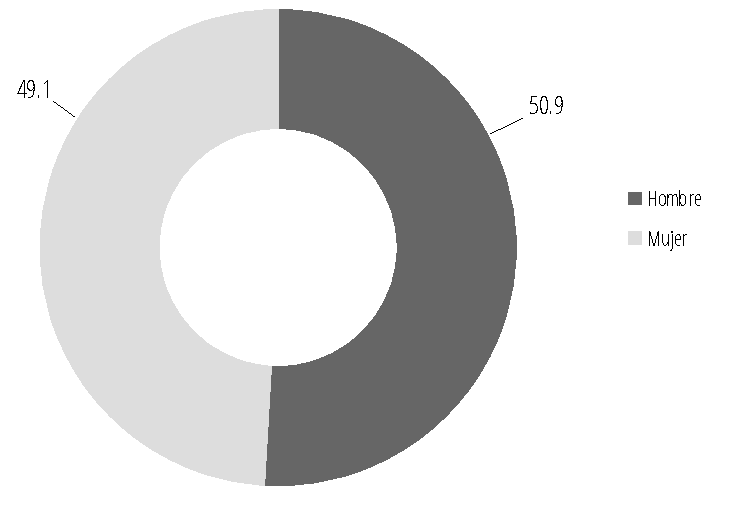
\includegraphics[width=22\cuadri]{1_07.pdf}}{INE, con datos del RENAP.}{}}
	{\columna{Nacimientos según peso del recién nacido}{El peso al nacer es una variable usada para evaluar las probabilidades de supervivencia del recién nacido en sus primeros días de vida, así como para evaluar las condiciones de las madres en una población.}{\quad En el primer trimestre del 2014, el 87.8\% del total de nacimientos registraron un peso adecuado al nacer (5.5 libras o más), mientras que en el 12.1\% de los casos, se registró bajo peso al nacer. Del total de nacimientos con bajo peso al nacer,  0.4\% presentan muy bajo peso al nacer (menos de 3.3 libras) y 0.2\% extremadamente bajo peso al nacer (menos de 2.2 libras).}{Distribución de nacimientos por peso del recién nacido}{Primer trimestre, año 2014}{\ \\[6mm]\begin{tikzpicture}[x=1pt,y=1pt,scale=0.90]  % Created by tikzDevice version 0.7.0 on 2014-12-03 22:07:12
% !TEX encoding = UTF-8 Unicode
\definecolor[named]{fillColor}{rgb}{1.00,1.00,1.00}
\path[use as bounding box,fill=fillColor,fill opacity=0.00] (0,0) rectangle (280.41,195.13);
\begin{scope}
\path[clip] (  0.00,  0.00) rectangle (280.41,195.13);
\definecolor[named]{drawColor}{rgb}{1.00,1.00,1.00}

\path[draw=drawColor,line width= 0.6pt,line join=round,line cap=round] ( -0.00,  0.00) rectangle (280.41,195.13);
\end{scope}
\begin{scope}
\path[clip] (  0.00,  0.00) rectangle (280.41,195.13);

\path[] ( 88.47, -1.53) rectangle (253.09,195.13);

\path[] ( 88.47, 14.85) --
	(253.09, 14.85);

\path[] ( 88.47, 42.17) --
	(253.09, 42.17);

\path[] ( 88.47, 69.48) --
	(253.09, 69.48);

\path[] ( 88.47, 96.80) --
	(253.09, 96.80);

\path[] ( 88.47,124.11) --
	(253.09,124.11);

\path[] ( 88.47,151.43) --
	(253.09,151.43);

\path[] ( 88.47,178.74) --
	(253.09,178.74);
\definecolor[named]{fillColor}{rgb}{0.86,0.68,0.43}

\path[fill=fillColor] ( 88.47,  6.66) rectangle ( 96.40, 23.05);

\path[fill=fillColor] ( 88.47, 33.97) rectangle (114.27, 50.36);

\path[fill=fillColor] ( 88.47, 61.29) rectangle (128.41, 77.68);

\path[fill=fillColor] ( 88.47, 88.60) rectangle (138.32,104.99);

\path[fill=fillColor] ( 88.47,115.92) rectangle (141.46,132.31);

\path[fill=fillColor] ( 88.47,143.23) rectangle (145.52,159.62);

\path[fill=fillColor] ( 88.47,170.55) rectangle (253.09,186.93);
\definecolor[named]{drawColor}{rgb}{0.00,0.00,0.00}

\node[text=drawColor,anchor=base west,inner sep=0pt, outer sep=0pt, scale=  0.71] at (102.64, 11.93) {835};

\node[text=drawColor,anchor=base west,inner sep=0pt, outer sep=0pt, scale=  0.71] at (122.59, 39.24) {2718};

\node[text=drawColor,anchor=base west,inner sep=0pt, outer sep=0pt, scale=  0.71] at (136.73, 66.55) {4208};

\node[text=drawColor,anchor=base west,inner sep=0pt, outer sep=0pt, scale=  0.71] at (146.65, 93.87) {5253};

\node[text=drawColor,anchor=base west,inner sep=0pt, outer sep=0pt, scale=  0.71] at (149.78,121.18) {5583};

\node[text=drawColor,anchor=base west,inner sep=0pt, outer sep=0pt, scale=  0.71] at (153.84,148.50) {6011};

\node[text=drawColor,anchor=base west,inner sep=0pt, outer sep=0pt, scale=  0.71] at (263.50,175.81) {17346};
\end{scope}
\begin{scope}
\path[clip] (  0.00,  0.00) rectangle (280.41,195.13);
\definecolor[named]{drawColor}{rgb}{0.60,0.60,0.60}

\path[draw=drawColor,line width= 0.6pt,line join=round] ( 88.47,  0.00) --
	( 88.47,195.13);
\end{scope}
\begin{scope}
\path[clip] (  0.00,  0.00) rectangle (280.41,195.13);
\definecolor[named]{drawColor}{rgb}{0.00,0.00,0.00}

\node[text=drawColor,anchor=base east,inner sep=0pt, outer sep=0pt, scale=  0.83] at ( 81.36, 11.41) {Contra la sexualidad};

\node[text=drawColor,anchor=base east,inner sep=0pt, outer sep=0pt, scale=  0.83] at ( 81.36, 38.72) {Otras causas};

\node[text=drawColor,anchor=base east,inner sep=0pt, outer sep=0pt, scale=  0.83] at ( 81.36, 66.04) {Contra la libertad};

\node[text=drawColor,anchor=base east,inner sep=0pt, outer sep=0pt, scale=  0.83] at ( 81.36, 93.35) {Homicidios};

\node[text=drawColor,anchor=base east,inner sep=0pt, outer sep=0pt, scale=  0.83] at ( 81.36,120.67) {Extorsión y chantaje};

\node[text=drawColor,anchor=base east,inner sep=0pt, outer sep=0pt, scale=  0.83] at ( 81.36,147.98) {Lesiones};

\node[text=drawColor,anchor=base east,inner sep=0pt, outer sep=0pt, scale=  0.83] at ( 81.36,175.30) {Contra el patrimonio};
\end{scope}
\begin{scope}
\path[clip] (  0.00,  0.00) rectangle (280.41,195.13);

\path[] ( 84.20, 14.85) --
	( 88.47, 14.85);

\path[] ( 84.20, 42.17) --
	( 88.47, 42.17);

\path[] ( 84.20, 69.48) --
	( 88.47, 69.48);

\path[] ( 84.20, 96.80) --
	( 88.47, 96.80);

\path[] ( 84.20,124.11) --
	( 88.47,124.11);

\path[] ( 84.20,151.43) --
	( 88.47,151.43);

\path[] ( 84.20,178.74) --
	( 88.47,178.74);
\end{scope}
  \end{tikzpicture}}{INE, con datos del RENAP.}{}}
\hojados
	{\columna{Nacimientos con bajo peso al nacer}{Un bajo peso al nacer predispone al recién nacido a complicaciones de salud en los primeros días de vida.}{\quad Se puede observar que en los últimos dos años, el porcentaje de nacimientos registrados con bajo peso  al nacer, ha variado entre 11\% y 12.1\%. A partir del primer trimestre del  2012, el porcentaje se ha ido incrementando levemente, el mayor aumento se observó entre el primer y segundo trimestre del 2012 con 4.7\%. Entre último trimestre del 2013 y el primero del 2014, el aumento fue del 4.4\%.}{Porcentaje de nacimientos con bajo peso al nacer}{Serie histórica 2012-2014}{\ \\[6mm]\begin{tikzpicture}[x=1pt,y=1pt,scale=0.90]  % Created by tikzDevice version 0.7.0 on 2014-11-24 15:12:07
% !TEX encoding = UTF-8 Unicode
\definecolor[named]{fillColor}{rgb}{1.00,1.00,1.00}
\path[use as bounding box,fill=fillColor,fill opacity=0.00] (0,0) rectangle (280.41,195.13);
\begin{scope}
\path[clip] (  0.00,  0.00) rectangle (280.41,195.13);
\definecolor[named]{drawColor}{rgb}{1.00,1.00,1.00}

\path[draw=drawColor,line width= 0.6pt,line join=round,line cap=round] (  0.00,  0.00) rectangle (280.41,195.13);
\end{scope}
\begin{scope}
\path[clip] (  0.00,  0.00) rectangle (280.41,195.13);

\path[] ( -1.76, 14.00) rectangle (271.87,188.02);

\path[] (  0.00, 21.72) --
	(271.87, 21.72);

\path[] (  0.00, 67.02) --
	(271.87, 67.02);

\path[] (  0.00,112.33) --
	(271.87,112.33);

\path[] (  0.00,157.63) --
	(271.87,157.63);

\path[] ( 41.77, 14.00) --
	( 41.77,188.02);

\path[] (103.96, 14.00) --
	(103.96,188.02);

\path[] (166.15, 14.00) --
	(166.15,188.02);

\path[] (228.34, 14.00) --
	(228.34,188.02);

\path[] (  0.00, 44.37) --
	(271.87, 44.37);

\path[] (  0.00, 89.68) --
	(271.87, 89.68);

\path[] (  0.00,134.98) --
	(271.87,134.98);

\path[] (  0.00,180.29) --
	(271.87,180.29);

\path[] ( 10.68, 14.00) --
	( 10.68,188.02);

\path[] ( 72.87, 14.00) --
	( 72.87,188.02);

\path[] (135.06, 14.00) --
	(135.06,188.02);

\path[] (197.24, 14.00) --
	(197.24,188.02);

\path[] (259.43, 14.00) --
	(259.43,188.02);
\definecolor[named]{drawColor}{rgb}{0.86,0.68,0.43}

\path[draw=drawColor,line width= 1.9pt,line join=round] ( 10.68,180.11) --
	( 72.87,131.36) --
	(135.06,106.08) --
	(197.24, 58.42) --
	(259.43, 67.30);
\definecolor[named]{drawColor}{rgb}{0.00,0.00,0.00}

\node[text=drawColor,anchor=base,inner sep=0pt, outer sep=0pt, scale=  0.76] at ( 10.68,183.23) {6,498.0};

\node[text=drawColor,anchor=base west,inner sep=0pt, outer sep=0pt, scale=  0.76] at ( 72.87,134.48) {5,960.0};

\node[text=drawColor,anchor=base west,inner sep=0pt, outer sep=0pt, scale=  0.76] at (135.06,109.20) {5,681.0};

\node[text=drawColor,anchor=base,inner sep=0pt, outer sep=0pt, scale=  0.76] at (197.24, 49.05) {5,155.0};

\node[text=drawColor,anchor=base,inner sep=0pt, outer sep=0pt, scale=  0.76] at (259.43, 70.42) {5,253.0};
\end{scope}
\begin{scope}
\path[clip] (  0.00,  0.00) rectangle (280.41,195.13);
\definecolor[named]{drawColor}{rgb}{0.60,0.60,0.60}

\path[draw=drawColor,line width= 0.6pt,line join=round] (  0.00, 14.00) --
	(271.87, 14.00);
\end{scope}
\begin{scope}
\path[clip] (  0.00,  0.00) rectangle (280.41,195.13);

\path[] ( 10.68,  9.73) --
	( 10.68, 14.00);

\path[] ( 72.87,  9.73) --
	( 72.87, 14.00);

\path[] (135.06,  9.73) --
	(135.06, 14.00);

\path[] (197.24,  9.73) --
	(197.24, 14.00);

\path[] (259.43,  9.73) --
	(259.43, 14.00);
\end{scope}
\begin{scope}
\path[clip] (  0.00,  0.00) rectangle (280.41,195.13);
\definecolor[named]{drawColor}{rgb}{0.00,0.00,0.00}

\node[text=drawColor,anchor=base west,inner sep=0pt, outer sep=0pt, scale=  0.83] at ( 10.68, -0.00) {2009};

\node[text=drawColor,anchor=base west,inner sep=0pt, outer sep=0pt, scale=  0.83] at ( 72.87, -0.00) {2010};

\node[text=drawColor,anchor=base west,inner sep=0pt, outer sep=0pt, scale=  0.83] at (135.06, -0.00) {2011};

\node[text=drawColor,anchor=base west,inner sep=0pt, outer sep=0pt, scale=  0.83] at (197.24, -0.00) {2012};

\node[text=drawColor,anchor=base west,inner sep=0pt, outer sep=0pt, scale=  0.83] at (259.43, -0.00) {2013};
\end{scope}
  \end{tikzpicture}}{INE, con datos del RENAP.}{}}
	{\columna{Nacimientos por asistencia recibida durante el parto}{Una adecuada atención al momento del nacimiento garantiza la salud materna e infantil de una población.}{\quad Del total de nacimientos registrados durante el primer trimestre del 2014, el 65.3\% de los casos recibieron asistencia médica, el 30.7\% por comadrona, 1.4\% empírica y menos del 1\% recibió asistencia paramédica. En  1.7\% de los casos, no se recibió ninguna asistencia durante el parto.}{Distribución de nacimientos por asistencia recibida durante el parto}{Primer trimestre, año 2014}{\ \\[6mm]\begin{tikzpicture}[x=1pt,y=1pt,scale=0.90]  % Created by tikzDevice version 0.7.0 on 2014-12-11 15:14:28
% !TEX encoding = UTF-8 Unicode
\definecolor[named]{fillColor}{rgb}{1.00,1.00,1.00}
\path[use as bounding box,fill=fillColor,fill opacity=0.00] (0,0) rectangle (230.54,138.04);
\begin{scope}
\path[clip] (  0.00,  0.00) rectangle (230.54,138.04);
\definecolor[named]{drawColor}{rgb}{1.00,1.00,1.00}

\path[draw=drawColor,line width= 0.6pt,line join=round,line cap=round] (  0.00,  0.00) rectangle (230.54,138.04);
\end{scope}
\begin{scope}
\path[clip] (  0.00,  0.00) rectangle (230.54,138.04);

\path[] (  7.00, 28.11) rectangle (230.54,123.81);

\path[] ( 32.79, 28.11) --
	( 32.79,123.81);

\path[] ( 75.78, 28.11) --
	( 75.78,123.81);

\path[] (118.77, 28.11) --
	(118.77,123.81);

\path[] (161.76, 28.11) --
	(161.76,123.81);

\path[] (204.75, 28.11) --
	(204.75,123.81);
\definecolor[named]{drawColor}{rgb}{0.00,0.00,0.00}

\path[draw=drawColor,line width= 0.6pt,line join=round] ( 19.90, 28.11) rectangle ( 45.69,123.81);

\path[draw=drawColor,line width= 0.6pt,line join=round] ( 62.89, 28.11) rectangle ( 88.68, 73.17);

\path[draw=drawColor,line width= 0.6pt,line join=round] (105.87, 28.11) rectangle (131.67, 30.59);

\path[draw=drawColor,line width= 0.6pt,line join=round] (148.86, 28.11) rectangle (174.66, 30.10);

\path[draw=drawColor,line width= 0.6pt,line join=round] (191.85, 28.11) rectangle (217.64, 29.43);

\node[text=drawColor,anchor=base,inner sep=0pt, outer sep=0pt, scale=  0.71] at ( 32.79,126.74) {65.3};

\node[text=drawColor,anchor=base,inner sep=0pt, outer sep=0pt, scale=  0.71] at ( 75.78, 76.09) {30.7};

\node[text=drawColor,anchor=base,inner sep=0pt, outer sep=0pt, scale=  0.71] at (118.77, 33.52) {1.7};

\node[text=drawColor,anchor=base,inner sep=0pt, outer sep=0pt, scale=  0.71] at (161.76, 33.03) {1.4};

\node[text=drawColor,anchor=base,inner sep=0pt, outer sep=0pt, scale=  0.71] at (204.75, 32.36) {0.9};
\end{scope}
\begin{scope}
\path[clip] (  0.00,  0.00) rectangle (230.54,138.04);

\path[] (  7.00, 28.11) --
	(  7.00,123.81);
\end{scope}
\begin{scope}
\path[clip] (  0.00,  0.00) rectangle (230.54,138.04);
\definecolor[named]{drawColor}{rgb}{0.00,0.00,0.00}

\path[draw=drawColor,line width= 0.6pt,line join=round] (  7.00, 28.11) --
	(230.54, 28.11);
\end{scope}
\begin{scope}
\path[clip] (  0.00,  0.00) rectangle (230.54,138.04);

\path[] ( 32.79, 23.85) --
	( 32.79, 28.11);

\path[] ( 75.78, 23.85) --
	( 75.78, 28.11);

\path[] (118.77, 23.85) --
	(118.77, 28.11);

\path[] (161.76, 23.85) --
	(161.76, 28.11);

\path[] (204.75, 23.85) --
	(204.75, 28.11);
\end{scope}
\begin{scope}
\path[clip] (  0.00,  0.00) rectangle (230.54,138.04);
\definecolor[named]{drawColor}{rgb}{0.00,0.00,0.00}

\node[text=drawColor,anchor=base,inner sep=0pt, outer sep=0pt, scale=  0.83] at ( 32.79, 14.11) {Médica};

\node[text=drawColor,anchor=base,inner sep=0pt, outer sep=0pt, scale=  0.83] at ( 75.78, 14.11) {Comadrona};

\node[text=drawColor,anchor=base,inner sep=0pt, outer sep=0pt, scale=  0.83] at (118.77, 14.11) {Ninguna};

\node[text=drawColor,anchor=base,inner sep=0pt, outer sep=0pt, scale=  0.83] at (161.76, 14.11) {Empírica};

\node[text=drawColor,anchor=base,inner sep=0pt, outer sep=0pt, scale=  0.83] at (204.75, 14.11) {Paramédica};
\end{scope}
  \end{tikzpicture}}{INE, con datos del RENAP.}{}}



\INEchapter{Defunciones}{Defunciones}{}{\quad Es la desaparición permanente de todo signo de vida, cualquiera que sea el tiempo transcurrido desde el nacimiento vivo.}


\hojados{\columna{Defunciones}{Como se muestra en la gráfica de la serie histórica de defunciones, durante el primer trimestre del 2014 se registraron 18,445, 3,5\% menos que lo registrado en el mismo período del año anterior y 4\% menos que lo registrado en el último trimestre del 2013. La mayor variación trimestral se observa entre el tercer y cuarto trimestre del 2012 con un aumento del 7.3\%.  \\
		
		\quad Los datos se presentan como preliminares y serán ajustados por el registro tardío de los mismos.}{}{Defunciones por trimestre}{Serie histórica 2012-2014}{\ \\[5mm] \begin{tikzpicture}[x=1pt,y=1pt,scale=0.90]  % Created by tikzDevice version 0.7.0 on 2014-12-03 22:08:06
% !TEX encoding = UTF-8 Unicode
\definecolor[named]{fillColor}{rgb}{1.00,1.00,1.00}
\path[use as bounding box,fill=fillColor,fill opacity=0.00] (0,0) rectangle (280.41,195.13);
\begin{scope}
\path[clip] (  0.00,  0.00) rectangle (280.41,195.13);
\definecolor[named]{drawColor}{rgb}{1.00,1.00,1.00}

\path[draw=drawColor,line width= 0.6pt,line join=round,line cap=round] (  0.00,  0.00) rectangle (280.41,195.13);
\end{scope}
\begin{scope}
\path[clip] (  0.00,  0.00) rectangle (280.41,195.13);

\path[] ( 11.67, 14.00) rectangle (271.87,188.02);

\path[] ( 11.67, 25.20) --
	(271.87, 25.20);

\path[] ( 11.67, 69.93) --
	(271.87, 69.93);

\path[] ( 11.67,114.66) --
	(271.87,114.66);

\path[] ( 11.67,159.38) --
	(271.87,159.38);

\path[] ( 53.07, 14.00) --
	( 53.07,188.02);

\path[] (112.20, 14.00) --
	(112.20,188.02);

\path[] (171.34, 14.00) --
	(171.34,188.02);

\path[] (230.48, 14.00) --
	(230.48,188.02);

\path[] ( 11.67, 47.57) --
	(271.87, 47.57);

\path[] ( 11.67, 92.29) --
	(271.87, 92.29);

\path[] ( 11.67,137.02) --
	(271.87,137.02);

\path[] ( 11.67,181.75) --
	(271.87,181.75);

\path[] ( 23.50, 14.00) --
	( 23.50,188.02);

\path[] ( 82.63, 14.00) --
	( 82.63,188.02);

\path[] (141.77, 14.00) --
	(141.77,188.02);

\path[] (200.91, 14.00) --
	(200.91,188.02);

\path[] (260.04, 14.00) --
	(260.04,188.02);
\definecolor[named]{drawColor}{rgb}{0.86,0.68,0.43}

\path[draw=drawColor,line width= 1.9pt,line join=round] ( 23.50, 62.74) --
	( 82.63, 60.92) --
	(141.77, 58.42) --
	(200.91,154.78) --
	(260.04,180.11);
\definecolor[named]{drawColor}{rgb}{0.00,0.00,0.00}

\node[text=drawColor,anchor=base,inner sep=0pt, outer sep=0pt, scale=  0.76] at ( 23.50, 65.87) {23,393};

\node[text=drawColor,anchor=base west,inner sep=0pt, outer sep=0pt, scale=  0.76] at ( 82.63, 64.04) {22,985};

\node[text=drawColor,anchor=base,inner sep=0pt, outer sep=0pt, scale=  0.76] at (141.77, 49.05) {22,426};

\node[text=drawColor,anchor=base east,inner sep=0pt, outer sep=0pt, scale=  0.76] at (195.97,154.78) {43,970};

\node[text=drawColor,anchor=base,inner sep=0pt, outer sep=0pt, scale=  0.76] at (260.04,183.23) {49,633};
\end{scope}
\begin{scope}
\path[clip] (  0.00,  0.00) rectangle (280.41,195.13);

\path[] ( 11.67, 14.00) --
	( 11.67,188.02);
\end{scope}
\begin{scope}
\path[clip] (  0.00,  0.00) rectangle (280.41,195.13);
\definecolor[named]{drawColor}{rgb}{1.00,1.00,1.00}

\node[text=drawColor,text opacity=0.00,anchor=base east,inner sep=0pt, outer sep=0pt, scale=  0.83] at (  4.56, 44.12) {20000};

\node[text=drawColor,text opacity=0.00,anchor=base east,inner sep=0pt, outer sep=0pt, scale=  0.83] at (  4.56, 88.85) {30000};

\node[text=drawColor,text opacity=0.00,anchor=base east,inner sep=0pt, outer sep=0pt, scale=  0.83] at (  4.56,133.58) {40000};

\node[text=drawColor,text opacity=0.00,anchor=base east,inner sep=0pt, outer sep=0pt, scale=  0.83] at (  4.56,178.30) {50000};
\end{scope}
\begin{scope}
\path[clip] (  0.00,  0.00) rectangle (280.41,195.13);

\path[] (  7.40, 47.57) --
	( 11.67, 47.57);

\path[] (  7.40, 92.29) --
	( 11.67, 92.29);

\path[] (  7.40,137.02) --
	( 11.67,137.02);

\path[] (  7.40,181.75) --
	( 11.67,181.75);
\end{scope}
\begin{scope}
\path[clip] (  0.00,  0.00) rectangle (280.41,195.13);
\definecolor[named]{drawColor}{rgb}{0.60,0.60,0.60}

\path[draw=drawColor,line width= 0.6pt,line join=round] ( 11.67, 14.00) --
	(271.87, 14.00);
\end{scope}
\begin{scope}
\path[clip] (  0.00,  0.00) rectangle (280.41,195.13);

\path[] ( 23.50,  9.73) --
	( 23.50, 14.00);

\path[] ( 82.63,  9.73) --
	( 82.63, 14.00);

\path[] (141.77,  9.73) --
	(141.77, 14.00);

\path[] (200.91,  9.73) --
	(200.91, 14.00);

\path[] (260.04,  9.73) --
	(260.04, 14.00);
\end{scope}
\begin{scope}
\path[clip] (  0.00,  0.00) rectangle (280.41,195.13);
\definecolor[named]{drawColor}{rgb}{0.00,0.00,0.00}

\node[text=drawColor,anchor=base,inner sep=0pt, outer sep=0pt, scale=  0.83] at ( 23.50, -0.00) {2009};

\node[text=drawColor,anchor=base,inner sep=0pt, outer sep=0pt, scale=  0.83] at ( 82.63, -0.00) {2010};

\node[text=drawColor,anchor=base,inner sep=0pt, outer sep=0pt, scale=  0.83] at (141.77, -0.00) {2011};

\node[text=drawColor,anchor=base,inner sep=0pt, outer sep=0pt, scale=  0.83] at (200.91, -0.00) {2012};

\node[text=drawColor,anchor=base,inner sep=0pt, outer sep=0pt, scale=  0.83] at (260.04, -0.00) {2013};
\end{scope}
  \end{tikzpicture}}{INE, con datos del RENAP.}{}}
{\columna{Defunciones por departamento}{Como se observa en la gráfica, en el departamento de Guatemala residían la mayor proporción de personas
fallecidas durante el primer trimestre del 2014 (23.4\%). Le siguen los departamentos de Alta Verapaz y San Marcos con 5.8\% y 5.6\%, respectivamente. \\

\quad En el extremo inferior se encuentran los departamentos de El Progreso con 1.4\% y Baja Verapaz con 1.6\%.}{}{Número de defunciones por departamento de residencia de la persona fallecida}{Primer trimestre, año 2014}{\ \\[6mm]\begin{tikzpicture}[x=1pt,y=1pt,scale=0.90]  % Created by tikzDevice version 0.7.0 on 2014-12-03 22:08:08
% !TEX encoding = UTF-8 Unicode
\definecolor[named]{fillColor}{rgb}{1.00,1.00,1.00}
\path[use as bounding box,fill=fillColor,fill opacity=0.00] (0,0) rectangle (280.41,195.13);
\begin{scope}
\path[clip] (  0.00,  0.00) rectangle (280.41,195.13);
\definecolor[named]{drawColor}{rgb}{1.00,1.00,1.00}

\path[draw=drawColor,line width= 0.6pt,line join=round,line cap=round] (  0.00,  0.00) rectangle (280.41,195.13);
\end{scope}
\begin{scope}
\path[clip] (  0.00,  0.00) rectangle (280.41,195.13);

\path[] (  7.00, 65.36) rectangle (280.41,180.90);

\path[] ( 14.39, 65.36) --
	( 14.39,180.90);

\path[] ( 26.71, 65.36) --
	( 26.71,180.90);

\path[] ( 39.02, 65.36) --
	( 39.02,180.90);

\path[] ( 51.34, 65.36) --
	( 51.34,180.90);

\path[] ( 63.65, 65.36) --
	( 63.65,180.90);

\path[] ( 75.97, 65.36) --
	( 75.97,180.90);

\path[] ( 88.28, 65.36) --
	( 88.28,180.90);

\path[] (100.60, 65.36) --
	(100.60,180.90);

\path[] (112.92, 65.36) --
	(112.92,180.90);

\path[] (125.23, 65.36) --
	(125.23,180.90);

\path[] (137.55, 65.36) --
	(137.55,180.90);

\path[] (149.86, 65.36) --
	(149.86,180.90);

\path[] (162.18, 65.36) --
	(162.18,180.90);

\path[] (174.49, 65.36) --
	(174.49,180.90);

\path[] (186.81, 65.36) --
	(186.81,180.90);

\path[] (199.12, 65.36) --
	(199.12,180.90);

\path[] (211.44, 65.36) --
	(211.44,180.90);

\path[] (223.76, 65.36) --
	(223.76,180.90);

\path[] (236.07, 65.36) --
	(236.07,180.90);

\path[] (248.39, 65.36) --
	(248.39,180.90);

\path[] (260.70, 65.36) --
	(260.70,180.90);

\path[] (273.02, 65.36) --
	(273.02,180.90);
\definecolor[named]{fillColor}{rgb}{0.86,0.68,0.43}

\path[fill=fillColor] ( 10.70, 65.36) rectangle ( 18.09,180.90);

\path[fill=fillColor] ( 23.01, 65.36) rectangle ( 30.40, 93.72);

\path[fill=fillColor] ( 35.33, 65.36) rectangle ( 42.72, 93.31);

\path[fill=fillColor] ( 47.64, 65.36) rectangle ( 55.03, 90.80);

\path[fill=fillColor] ( 59.96, 65.36) rectangle ( 67.35, 85.80);

\path[fill=fillColor] ( 72.27, 65.36) rectangle ( 79.66, 84.96);

\path[fill=fillColor] ( 84.59, 65.36) rectangle ( 91.98, 82.04);

\path[fill=fillColor] ( 96.90, 65.36) rectangle (104.29, 82.04);

\path[fill=fillColor] (109.22, 65.36) rectangle (116.61, 81.21);

\path[fill=fillColor] (121.54, 65.36) rectangle (128.93, 79.96);

\path[fill=fillColor] (133.85, 65.36) rectangle (141.24, 79.96);

\path[fill=fillColor] (146.17, 65.36) rectangle (153.56, 78.71);

\path[fill=fillColor] (158.48, 65.36) rectangle (165.87, 76.62);

\path[fill=fillColor] (170.80, 65.36) rectangle (178.19, 76.20);

\path[fill=fillColor] (183.11, 65.36) rectangle (190.50, 75.37);

\path[fill=fillColor] (195.43, 65.36) rectangle (202.82, 75.37);

\path[fill=fillColor] (207.75, 65.36) rectangle (215.13, 75.37);

\path[fill=fillColor] (220.06, 65.36) rectangle (227.45, 74.53);

\path[fill=fillColor] (232.38, 65.36) rectangle (239.77, 73.70);

\path[fill=fillColor] (244.69, 65.36) rectangle (252.08, 72.45);

\path[fill=fillColor] (257.01, 65.36) rectangle (264.40, 72.45);

\path[fill=fillColor] (269.32, 65.36) rectangle (276.71, 69.11);
\definecolor[named]{drawColor}{rgb}{0.00,0.00,0.00}

\node[text=drawColor,anchor=base,inner sep=0pt, outer sep=0pt, scale=  0.71] at ( 14.39,183.83) {27.7};

\node[text=drawColor,anchor=base,inner sep=0pt, outer sep=0pt, scale=  0.71] at ( 26.71, 96.65) {6.8};

\node[text=drawColor,anchor=base,inner sep=0pt, outer sep=0pt, scale=  0.71] at ( 39.02, 96.23) {6.7};

\node[text=drawColor,anchor=base,inner sep=0pt, outer sep=0pt, scale=  0.71] at ( 51.34, 93.73) {6.1};

\node[text=drawColor,anchor=base,inner sep=0pt, outer sep=0pt, scale=  0.71] at ( 63.65, 88.73) {4.9};

\node[text=drawColor,anchor=base,inner sep=0pt, outer sep=0pt, scale=  0.71] at ( 75.97, 87.89) {4.7};

\node[text=drawColor,anchor=base,inner sep=0pt, outer sep=0pt, scale=  0.71] at ( 88.28, 84.97) {4.0};

\node[text=drawColor,anchor=base,inner sep=0pt, outer sep=0pt, scale=  0.71] at (100.60, 84.97) {4.0};

\node[text=drawColor,anchor=base,inner sep=0pt, outer sep=0pt, scale=  0.71] at (112.92, 84.14) {3.8};

\node[text=drawColor,anchor=base,inner sep=0pt, outer sep=0pt, scale=  0.71] at (125.23, 82.89) {3.5};

\node[text=drawColor,anchor=base,inner sep=0pt, outer sep=0pt, scale=  0.71] at (137.55, 82.89) {3.5};

\node[text=drawColor,anchor=base,inner sep=0pt, outer sep=0pt, scale=  0.71] at (149.86, 81.63) {3.2};

\node[text=drawColor,anchor=base,inner sep=0pt, outer sep=0pt, scale=  0.71] at (162.18, 79.55) {2.7};

\node[text=drawColor,anchor=base,inner sep=0pt, outer sep=0pt, scale=  0.71] at (174.49, 79.13) {2.6};

\node[text=drawColor,anchor=base,inner sep=0pt, outer sep=0pt, scale=  0.71] at (186.81, 78.30) {2.4};

\node[text=drawColor,anchor=base,inner sep=0pt, outer sep=0pt, scale=  0.71] at (199.12, 78.30) {2.4};

\node[text=drawColor,anchor=base,inner sep=0pt, outer sep=0pt, scale=  0.71] at (211.44, 78.30) {2.4};

\node[text=drawColor,anchor=base,inner sep=0pt, outer sep=0pt, scale=  0.71] at (223.76, 77.46) {2.2};

\node[text=drawColor,anchor=base,inner sep=0pt, outer sep=0pt, scale=  0.71] at (236.07, 76.63) {2.0};

\node[text=drawColor,anchor=base,inner sep=0pt, outer sep=0pt, scale=  0.71] at (248.39, 75.38) {1.7};

\node[text=drawColor,anchor=base,inner sep=0pt, outer sep=0pt, scale=  0.71] at (260.70, 75.38) {1.7};

\node[text=drawColor,anchor=base,inner sep=0pt, outer sep=0pt, scale=  0.71] at (273.02, 72.04) {0.9};
\end{scope}
\begin{scope}
\path[clip] (  0.00,  0.00) rectangle (280.41,195.13);

\path[] (  7.00, 65.36) --
	(  7.00,180.90);
\end{scope}
\begin{scope}
\path[clip] (  0.00,  0.00) rectangle (280.41,195.13);
\definecolor[named]{drawColor}{rgb}{0.60,0.60,0.60}

\path[draw=drawColor,line width= 0.6pt,line join=round] (  7.00, 65.36) --
	(280.41, 65.36);
\end{scope}
\begin{scope}
\path[clip] (  0.00,  0.00) rectangle (280.41,195.13);

\path[] ( 14.39, 61.09) --
	( 14.39, 65.36);

\path[] ( 26.71, 61.09) --
	( 26.71, 65.36);

\path[] ( 39.02, 61.09) --
	( 39.02, 65.36);

\path[] ( 51.34, 61.09) --
	( 51.34, 65.36);

\path[] ( 63.65, 61.09) --
	( 63.65, 65.36);

\path[] ( 75.97, 61.09) --
	( 75.97, 65.36);

\path[] ( 88.28, 61.09) --
	( 88.28, 65.36);

\path[] (100.60, 61.09) --
	(100.60, 65.36);

\path[] (112.92, 61.09) --
	(112.92, 65.36);

\path[] (125.23, 61.09) --
	(125.23, 65.36);

\path[] (137.55, 61.09) --
	(137.55, 65.36);

\path[] (149.86, 61.09) --
	(149.86, 65.36);

\path[] (162.18, 61.09) --
	(162.18, 65.36);

\path[] (174.49, 61.09) --
	(174.49, 65.36);

\path[] (186.81, 61.09) --
	(186.81, 65.36);

\path[] (199.12, 61.09) --
	(199.12, 65.36);

\path[] (211.44, 61.09) --
	(211.44, 65.36);

\path[] (223.76, 61.09) --
	(223.76, 65.36);

\path[] (236.07, 61.09) --
	(236.07, 65.36);

\path[] (248.39, 61.09) --
	(248.39, 65.36);

\path[] (260.70, 61.09) --
	(260.70, 65.36);

\path[] (273.02, 61.09) --
	(273.02, 65.36);
\end{scope}
\begin{scope}
\path[clip] (  0.00,  0.00) rectangle (280.41,195.13);
\definecolor[named]{drawColor}{rgb}{0.00,0.00,0.00}

\node[text=drawColor,rotate= 90.00,anchor=base east,inner sep=0pt, outer sep=0pt, scale=  0.83] at ( 17.83, 58.24) {Guatemala};

\node[text=drawColor,rotate= 90.00,anchor=base east,inner sep=0pt, outer sep=0pt, scale=  0.83] at ( 30.15, 58.24) {Quetzaltenango};

\node[text=drawColor,rotate= 90.00,anchor=base east,inner sep=0pt, outer sep=0pt, scale=  0.83] at ( 42.47, 58.24) {Escuintla};

\node[text=drawColor,rotate= 90.00,anchor=base east,inner sep=0pt, outer sep=0pt, scale=  0.83] at ( 54.78, 58.24) {Huehuetenango};

\node[text=drawColor,rotate= 90.00,anchor=base east,inner sep=0pt, outer sep=0pt, scale=  0.83] at ( 67.10, 58.24) {San Marcos};

\node[text=drawColor,rotate= 90.00,anchor=base east,inner sep=0pt, outer sep=0pt, scale=  0.83] at ( 79.41, 58.24) {Alta Verapaz};

\node[text=drawColor,rotate= 90.00,anchor=base east,inner sep=0pt, outer sep=0pt, scale=  0.83] at ( 91.73, 58.24) {Suchitepéquez};

\node[text=drawColor,rotate= 90.00,anchor=base east,inner sep=0pt, outer sep=0pt, scale=  0.83] at (104.04, 58.24) {Jutiapa};

\node[text=drawColor,rotate= 90.00,anchor=base east,inner sep=0pt, outer sep=0pt, scale=  0.83] at (116.36, 58.24) {Retalhuleu};

\node[text=drawColor,rotate= 90.00,anchor=base east,inner sep=0pt, outer sep=0pt, scale=  0.83] at (128.67, 58.24) {Quiché};

\node[text=drawColor,rotate= 90.00,anchor=base east,inner sep=0pt, outer sep=0pt, scale=  0.83] at (140.99, 58.24) {Santa Rosa};

\node[text=drawColor,rotate= 90.00,anchor=base east,inner sep=0pt, outer sep=0pt, scale=  0.83] at (153.31, 58.24) {Petén};

\node[text=drawColor,rotate= 90.00,anchor=base east,inner sep=0pt, outer sep=0pt, scale=  0.83] at (165.62, 58.24) {Jalapa};

\node[text=drawColor,rotate= 90.00,anchor=base east,inner sep=0pt, outer sep=0pt, scale=  0.83] at (177.94, 58.24) {Baja Verapaz};

\node[text=drawColor,rotate= 90.00,anchor=base east,inner sep=0pt, outer sep=0pt, scale=  0.83] at (190.25, 58.24) {Chiquimula};

\node[text=drawColor,rotate= 90.00,anchor=base east,inner sep=0pt, outer sep=0pt, scale=  0.83] at (202.57, 58.24) {Chimaltenango};

\node[text=drawColor,rotate= 90.00,anchor=base east,inner sep=0pt, outer sep=0pt, scale=  0.83] at (214.88, 58.24) {Izabal};

\node[text=drawColor,rotate= 90.00,anchor=base east,inner sep=0pt, outer sep=0pt, scale=  0.83] at (227.20, 58.24) {Sololá};

\node[text=drawColor,rotate= 90.00,anchor=base east,inner sep=0pt, outer sep=0pt, scale=  0.83] at (239.51, 58.24) {Sacatepéquez};

\node[text=drawColor,rotate= 90.00,anchor=base east,inner sep=0pt, outer sep=0pt, scale=  0.83] at (251.83, 58.24) {Zacapa};

\node[text=drawColor,rotate= 90.00,anchor=base east,inner sep=0pt, outer sep=0pt, scale=  0.83] at (264.15, 58.24) {El Progreso};

\node[text=drawColor,rotate= 90.00,anchor=base east,inner sep=0pt, outer sep=0pt, scale=  0.83] at (276.46, 58.24) {Totonicapán};
\end{scope}
  \end{tikzpicture}}{INE, con datos del RENAP.}{}}
\hojados{\columna{Defunciones por día de la semana}{En la gráfica de defunciones por día de la semana de ocurrencia, el día martes es cuando se registraron la menor cantidad de defunciones, 12.8\%.  El día en que ocurrieron la mayor cantidad de defunciones fue lunes con el 15.3\% de los casos, seguido de sábado y domingo, ambos con el 14.9\%.}{\quad Las defunciones por causas externas ocurren principalmente los días festivos y fines de semana.}{Distribución de defunciones por día de la semana de ocurrencia}{Primer trimestre, año 2014}{\ \\[6mm]\begin{tikzpicture}[x=1pt,y=1pt,scale=0.90]  % Created by tikzDevice version 0.7.0 on 2014-12-12 12:44:39
% !TEX encoding = UTF-8 Unicode
\definecolor[named]{fillColor}{rgb}{1.00,1.00,1.00}
\path[use as bounding box,fill=fillColor,fill opacity=0.00] (0,0) rectangle (230.54,138.04);
\begin{scope}
\path[clip] (  0.00,  0.00) rectangle (230.54,138.04);
\definecolor[named]{drawColor}{rgb}{1.00,1.00,1.00}

\path[draw=drawColor,line width= 0.6pt,line join=round,line cap=round] (  0.00,  0.00) rectangle (230.54,138.04);
\end{scope}
\begin{scope}
\path[clip] (  0.00,  0.00) rectangle (230.54,138.04);

\path[] (  7.00, 28.11) rectangle (230.54,123.81);

\path[] ( 25.63, 28.11) --
	( 25.63,123.81);

\path[] ( 56.68, 28.11) --
	( 56.68,123.81);

\path[] ( 87.72, 28.11) --
	( 87.72,123.81);

\path[] (118.77, 28.11) --
	(118.77,123.81);

\path[] (149.82, 28.11) --
	(149.82,123.81);

\path[] (180.87, 28.11) --
	(180.87,123.81);

\path[] (211.91, 28.11) --
	(211.91,123.81);
\definecolor[named]{drawColor}{rgb}{0.00,0.00,0.00}

\path[draw=drawColor,line width= 0.6pt,line join=round] ( 16.32, 28.11) rectangle ( 34.94,123.81);

\path[draw=drawColor,line width= 0.6pt,line join=round] ( 47.36, 28.11) rectangle ( 65.99,108.25);

\path[draw=drawColor,line width= 0.6pt,line join=round] ( 78.41, 28.11) rectangle ( 97.04,115.72);

\path[draw=drawColor,line width= 0.6pt,line join=round] (109.46, 28.11) rectangle (128.09,117.39);

\path[draw=drawColor,line width= 0.6pt,line join=round] (140.50, 28.11) rectangle (159.13,114.91);

\path[draw=drawColor,line width= 0.6pt,line join=round] (171.55, 28.11) rectangle (190.18,121.70);

\path[draw=drawColor,line width= 0.6pt,line join=round] (202.60, 28.11) rectangle (221.23,121.60);

\node[text=drawColor,anchor=base,inner sep=0pt, outer sep=0pt, scale=  0.71] at ( 25.63,126.74) {15.3};

\node[text=drawColor,anchor=base,inner sep=0pt, outer sep=0pt, scale=  0.71] at ( 56.68,111.18) {12.8};

\node[text=drawColor,anchor=base,inner sep=0pt, outer sep=0pt, scale=  0.71] at ( 87.72,118.65) {14.0};

\node[text=drawColor,anchor=base,inner sep=0pt, outer sep=0pt, scale=  0.71] at (118.77,120.32) {14.2};

\node[text=drawColor,anchor=base,inner sep=0pt, outer sep=0pt, scale=  0.71] at (149.82,117.84) {13.9};

\node[text=drawColor,anchor=base,inner sep=0pt, outer sep=0pt, scale=  0.71] at (180.87,124.63) {14.9};

\node[text=drawColor,anchor=base,inner sep=0pt, outer sep=0pt, scale=  0.71] at (211.91,124.53) {14.9};
\end{scope}
\begin{scope}
\path[clip] (  0.00,  0.00) rectangle (230.54,138.04);

\path[] (  7.00, 28.11) --
	(  7.00,123.81);
\end{scope}
\begin{scope}
\path[clip] (  0.00,  0.00) rectangle (230.54,138.04);
\definecolor[named]{drawColor}{rgb}{0.00,0.00,0.00}

\path[draw=drawColor,line width= 0.6pt,line join=round] (  7.00, 28.11) --
	(230.54, 28.11);
\end{scope}
\begin{scope}
\path[clip] (  0.00,  0.00) rectangle (230.54,138.04);

\path[] ( 25.63, 23.85) --
	( 25.63, 28.11);

\path[] ( 56.68, 23.85) --
	( 56.68, 28.11);

\path[] ( 87.72, 23.85) --
	( 87.72, 28.11);

\path[] (118.77, 23.85) --
	(118.77, 28.11);

\path[] (149.82, 23.85) --
	(149.82, 28.11);

\path[] (180.87, 23.85) --
	(180.87, 28.11);

\path[] (211.91, 23.85) --
	(211.91, 28.11);
\end{scope}
\begin{scope}
\path[clip] (  0.00,  0.00) rectangle (230.54,138.04);
\definecolor[named]{drawColor}{rgb}{0.00,0.00,0.00}

\node[text=drawColor,anchor=base,inner sep=0pt, outer sep=0pt, scale=  0.83] at ( 25.63, 14.11) {Lunes};

\node[text=drawColor,anchor=base,inner sep=0pt, outer sep=0pt, scale=  0.83] at ( 56.68, 14.11) {Martes};

\node[text=drawColor,anchor=base,inner sep=0pt, outer sep=0pt, scale=  0.83] at ( 87.72, 14.11) {Miércoles};

\node[text=drawColor,anchor=base,inner sep=0pt, outer sep=0pt, scale=  0.83] at (118.77, 14.11) {Jueves};

\node[text=drawColor,anchor=base,inner sep=0pt, outer sep=0pt, scale=  0.83] at (149.82, 14.11) {Viernes};

\node[text=drawColor,anchor=base,inner sep=0pt, outer sep=0pt, scale=  0.83] at (180.87, 14.11) {Sábado};

\node[text=drawColor,anchor=base,inner sep=0pt, outer sep=0pt, scale=  0.83] at (211.91, 14.11) {Domingo};
\end{scope}
  \end{tikzpicture}}{INE, con datos del RENAP.}{}}
{\columna{Mortalidad infantil}{Durante el primer trimestre del 2014 se registraron 1,750 defunciones de menores de un año, al desagregar por sexo se observa que del total de casos, el 58.2\% fueron hombres.\\
		
\quad En cuanto a la edad del menor al momento de la muerte (neonatal y post-neonatal), se observa que el 48.7\% falleció entre los primeros 27 días de nacido, mientras que el 51.3\% corresponde a la mortalidad ocurrida a partir de los 28 días, pero antes de cumplir el año.}{}{Defunciones neonatales y post neonatales por sexo}{Primer trimestre, año 2014}{\ \\[6mm]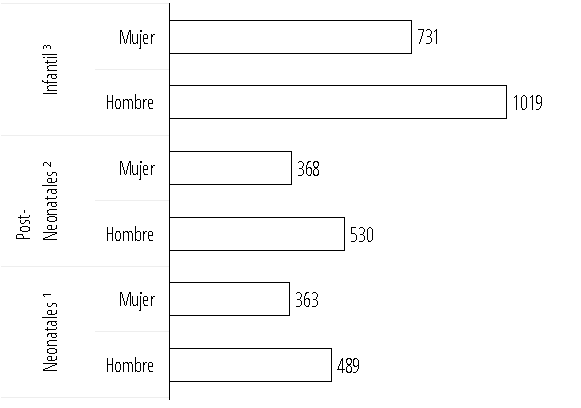
\includegraphics[width=22\cuadri]{2_04.pdf}}{INE, con datos del RENAP.}{\notitasin{ \textsuperscript{1} Niños menores de 28 días.} \notitasin{ \textsuperscript{2} Niños de 28 días o mayores, y menores a un año.} \notitasin{ \textsuperscript{3} Niños mayores a un año.}}}
\hojados{\columna{Defunciones en menores de cinco años}{La mortalidad en la niñez se considera como un indicador clave para poder determinar las condiciones básicas de salud de una población.}{\quad Como se muestra en la gráfica, el porcentaje de defunciones en menores de 5 años para el primer trimestre del 2014, representan el 12.6\%, esto es un aumento del 28.5\% de los casos en relación al último trimestre del 2013.  El dato más bajo de la serie corresponde al cuarto trimestre del 2013 (9.8\%) precisamente ese trimestre disminuyó un 29.9\% en relación al trimestre precedente.}{Porcentaje de defunciones en menores de cinco años}{Serie histórica 2012-2014}{\ \\[6mm]\begin{tikzpicture}[x=1pt,y=1pt,scale=0.90]  % Created by tikzDevice version 0.7.0 on 2014-11-24 15:15:07
% !TEX encoding = UTF-8 Unicode
\definecolor[named]{fillColor}{rgb}{1.00,1.00,1.00}
\path[use as bounding box,fill=fillColor,fill opacity=0.00] (0,0) rectangle (280.41,195.13);
\begin{scope}
\path[clip] (  0.00,  0.00) rectangle (280.41,195.13);
\definecolor[named]{drawColor}{rgb}{1.00,1.00,1.00}

\path[draw=drawColor,line width= 0.6pt,line join=round,line cap=round] (  0.00,  0.00) rectangle (280.41,195.13);
\end{scope}
\begin{scope}
\path[clip] (  0.00,  0.00) rectangle (280.41,195.13);

\path[] (  7.00, 28.11) rectangle (280.41,180.90);

\path[] ( 29.78, 28.11) --
	( 29.78,180.90);

\path[] ( 67.76, 28.11) --
	( 67.76,180.90);

\path[] (105.73, 28.11) --
	(105.73,180.90);

\path[] (143.70, 28.11) --
	(143.70,180.90);

\path[] (181.68, 28.11) --
	(181.68,180.90);

\path[] (219.65, 28.11) --
	(219.65,180.90);

\path[] (257.62, 28.11) --
	(257.62,180.90);
\definecolor[named]{fillColor}{rgb}{0.86,0.68,0.43}

\path[fill=fillColor] ( 18.39, 28.11) rectangle ( 41.18,133.71);

\path[fill=fillColor] ( 56.37, 28.11) rectangle ( 79.15,125.71);

\path[fill=fillColor] ( 94.34, 28.11) rectangle (117.12,132.11);

\path[fill=fillColor] (132.31, 28.11) rectangle (155.10,132.11);

\path[fill=fillColor] (170.29, 28.11) rectangle (193.07,136.11);

\path[fill=fillColor] (208.26, 28.11) rectangle (231.04,156.10);

\path[fill=fillColor] (246.23, 28.11) rectangle (269.02,180.90);
\definecolor[named]{drawColor}{rgb}{0.00,0.00,0.00}

\node[text=drawColor,anchor=base,inner sep=0pt, outer sep=0pt, scale=  0.71] at ( 29.78,136.63) {13.2};

\node[text=drawColor,anchor=base,inner sep=0pt, outer sep=0pt, scale=  0.71] at ( 67.76,128.64) {12.2};

\node[text=drawColor,anchor=base,inner sep=0pt, outer sep=0pt, scale=  0.71] at (105.73,135.03) {13.0};

\node[text=drawColor,anchor=base,inner sep=0pt, outer sep=0pt, scale=  0.71] at (143.70,135.03) {13.0};

\node[text=drawColor,anchor=base,inner sep=0pt, outer sep=0pt, scale=  0.71] at (181.68,139.03) {13.5};

\node[text=drawColor,anchor=base,inner sep=0pt, outer sep=0pt, scale=  0.71] at (219.65,159.03) {16.0};

\node[text=drawColor,anchor=base,inner sep=0pt, outer sep=0pt, scale=  0.71] at (257.62,183.83) {19.1};
\end{scope}
\begin{scope}
\path[clip] (  0.00,  0.00) rectangle (280.41,195.13);

\path[] (  7.00, 28.11) --
	(  7.00,180.90);
\end{scope}
\begin{scope}
\path[clip] (  0.00,  0.00) rectangle (280.41,195.13);
\definecolor[named]{drawColor}{rgb}{0.60,0.60,0.60}

\path[draw=drawColor,line width= 0.6pt,line join=round] (  7.00, 28.11) --
	(280.41, 28.11);
\end{scope}
\begin{scope}
\path[clip] (  0.00,  0.00) rectangle (280.41,195.13);

\path[] ( 29.78, 23.85) --
	( 29.78, 28.11);

\path[] ( 67.76, 23.85) --
	( 67.76, 28.11);

\path[] (105.73, 23.85) --
	(105.73, 28.11);

\path[] (143.70, 23.85) --
	(143.70, 28.11);

\path[] (181.68, 23.85) --
	(181.68, 28.11);

\path[] (219.65, 23.85) --
	(219.65, 28.11);

\path[] (257.62, 23.85) --
	(257.62, 28.11);
\end{scope}
\begin{scope}
\path[clip] (  0.00,  0.00) rectangle (280.41,195.13);
\definecolor[named]{drawColor}{rgb}{0.00,0.00,0.00}

\node[text=drawColor,anchor=base west,inner sep=0pt, outer sep=0pt, scale=  0.83] at ( 29.78, 14.11) {Lunes};

\node[text=drawColor,anchor=base west,inner sep=0pt, outer sep=0pt, scale=  0.83] at ( 67.76, 14.11) {Martes};

\node[text=drawColor,anchor=base west,inner sep=0pt, outer sep=0pt, scale=  0.83] at (105.73, 14.11) {Miercoles};

\node[text=drawColor,anchor=base west,inner sep=0pt, outer sep=0pt, scale=  0.83] at (143.70, 14.11) {Jueves};

\node[text=drawColor,anchor=base west,inner sep=0pt, outer sep=0pt, scale=  0.83] at (181.68, 14.11) {Viernes};

\node[text=drawColor,anchor=base west,inner sep=0pt, outer sep=0pt, scale=  0.83] at (219.65, 14.11) {Sabado};

\node[text=drawColor,anchor=base west,inner sep=0pt, outer sep=0pt, scale=  0.83] at (257.62, 14.11) {Domingo};
\end{scope}
  \end{tikzpicture}}{INE, con datos del RENAP.}{}}
{\columna{Defunciones según asistencia recibida}{La desagregación de las estadísticas según el tipo de asistencia recibida al momento de la defunción,  muestran que para el primer trimestre del 2014, en la mayoría de los casos, la persona fallecida no recibió ningún tipo de asistencia (51.7\% de los casos). En el 45.6\% de los casos recibieron asistencia médica y en 2.2\% asistencia empírica.\\
		
\quad Se registraron 69 casos que recibieron asistencia paramédica y 17 casos que recibieron asistencia de una
comadrona.}{}{Distribución de defunciones según asistencia recibida al momento de la defunción}{Primer trimestre, año 2014}{\ \\[6mm]\begin{tikzpicture}[x=1pt,y=1pt,scale=0.90]  % Created by tikzDevice version 0.7.0 on 2014-12-18 22:06:09
% !TEX encoding = UTF-8 Unicode
\definecolor[named]{fillColor}{rgb}{1.00,1.00,1.00}
\path[use as bounding box,fill=fillColor,fill opacity=0.00] (0,0) rectangle (230.54,138.04);
\begin{scope}
\path[clip] (  0.00,  0.00) rectangle (230.54,138.04);
\definecolor[named]{drawColor}{rgb}{1.00,1.00,1.00}

\path[draw=drawColor,line width= 0.6pt,line join=round,line cap=round] (  0.00,  0.00) rectangle (230.54,138.04);
\end{scope}
\begin{scope}
\path[clip] (  0.00,  0.00) rectangle (230.54,138.04);

\path[] (  6.05, 27.41) rectangle (230.54,123.81);

\path[] ( 31.95, 27.41) --
	( 31.95,123.81);

\path[] ( 75.12, 27.41) --
	( 75.12,123.81);

\path[] (118.29, 27.41) --
	(118.29,123.81);

\path[] (161.47, 27.41) --
	(161.47,123.81);

\path[] (204.64, 27.41) --
	(204.64,123.81);
\definecolor[named]{drawColor}{rgb}{0.00,0.00,0.00}

\path[draw=drawColor,line width= 0.6pt,line join=round] ( 19.00, 27.41) rectangle ( 44.90,123.81);

\path[draw=drawColor,line width= 0.6pt,line join=round] ( 62.17, 27.41) rectangle ( 88.07,112.44);

\path[draw=drawColor,line width= 0.6pt,line join=round] (105.34, 27.41) rectangle (131.25, 31.51);

\path[draw=drawColor,line width= 0.6pt,line join=round] (148.51, 27.41) rectangle (174.42, 28.16);

\path[draw=drawColor,line width= 0.6pt,line join=round] (191.69, 27.41) rectangle (217.59, 27.60);

\node[text=drawColor,anchor=base,inner sep=0pt, outer sep=0pt, scale=  0.85] at ( 31.95,126.84) {51.7};

\node[text=drawColor,anchor=base,inner sep=0pt, outer sep=0pt, scale=  0.85] at ( 75.12,115.47) {45.6};

\node[text=drawColor,anchor=base,inner sep=0pt, outer sep=0pt, scale=  0.85] at (118.29, 34.55) {2.2};

\node[text=drawColor,anchor=base,inner sep=0pt, outer sep=0pt, scale=  0.85] at (161.47, 31.19) {0.4};

\node[text=drawColor,anchor=base,inner sep=0pt, outer sep=0pt, scale=  0.85] at (204.64, 30.63) {0.1};
\end{scope}
\begin{scope}
\path[clip] (  0.00,  0.00) rectangle (230.54,138.04);

\path[] (  6.05, 27.41) --
	(  6.05,123.81);
\end{scope}
\begin{scope}
\path[clip] (  0.00,  0.00) rectangle (230.54,138.04);
\definecolor[named]{drawColor}{rgb}{0.00,0.00,0.00}

\path[draw=drawColor,line width= 0.6pt,line join=round] (  6.05, 27.41) --
	(230.54, 27.41);
\end{scope}
\begin{scope}
\path[clip] (  0.00,  0.00) rectangle (230.54,138.04);

\path[] ( 31.95, 23.15) --
	( 31.95, 27.41);

\path[] ( 75.12, 23.15) --
	( 75.12, 27.41);

\path[] (118.29, 23.15) --
	(118.29, 27.41);

\path[] (161.47, 23.15) --
	(161.47, 27.41);

\path[] (204.64, 23.15) --
	(204.64, 27.41);
\end{scope}
\begin{scope}
\path[clip] (  0.00,  0.00) rectangle (230.54,138.04);
\definecolor[named]{drawColor}{rgb}{0.00,0.00,0.00}

\node[text=drawColor,anchor=base,inner sep=0pt, outer sep=0pt, scale=  1.00] at ( 31.95, 13.16) {Ninguna};

\node[text=drawColor,anchor=base,inner sep=0pt, outer sep=0pt, scale=  1.00] at ( 75.12, 13.16) {Médica};

\node[text=drawColor,anchor=base,inner sep=0pt, outer sep=0pt, scale=  1.00] at (118.29, 13.16) {Empírica};

\node[text=drawColor,anchor=base,inner sep=0pt, outer sep=0pt, scale=  1.00] at (161.47, 13.16) {Paramédica};

\node[text=drawColor,anchor=base,inner sep=0pt, outer sep=0pt, scale=  1.00] at (204.64, 13.16) {Comadrona};
\end{scope}
  \end{tikzpicture}}{INE, con datos del RENAP.}{}}
\hojados{\columna{Defunciones por lugar de ocurrencia}{El lugar de ocurrencia de una defunción está estrechamente relacionado con la atención recibida y las condiciones de la misma.}{\quad Como se advierte en la gráfica de defunciones por lugar de ocurrencia, en el 60.4\% de los casos, las defunciones ocurrieron en el domicilio de la persona fallecida, en el 29.2\% de los casos, en un hospital o centro de salud, registrándose la mayor proporción en un hospital público. 698 defunciones equivalente al 3.8\%, ocurrieron en la vía pública y 1.1\% en otro lugar. Se ignora el lugar de ocurrencia del 5.5\% de las defunciones.}{Distribución de defunciones por lugar de ocurrencia}{Primer trimestre, año 2014}{\ \\[6mm]\begin{tikzpicture}[x=1pt,y=1pt,scale=0.90]  % Created by tikzDevice version 0.7.0 on 2014-12-18 22:06:14
% !TEX encoding = UTF-8 Unicode
\definecolor[named]{fillColor}{rgb}{1.00,1.00,1.00}
\path[use as bounding box,fill=fillColor,fill opacity=0.00] (0,0) rectangle (230.54,138.04);
\begin{scope}
\path[clip] (  0.00,  0.00) rectangle (230.54,138.04);
\definecolor[named]{drawColor}{rgb}{1.00,1.00,1.00}

\path[draw=drawColor,line width= 0.6pt,line join=round,line cap=round] (  0.00,  0.00) rectangle (230.54,138.04);
\end{scope}
\begin{scope}
\path[clip] (  0.00,  0.00) rectangle (230.54,138.04);

\path[] ( 60.02, -2.49) rectangle (206.64,138.04);

\path[] ( 60.02,  6.68) --
	(206.64,  6.68);

\path[] ( 60.02, 21.95) --
	(206.64, 21.95);

\path[] ( 60.02, 37.23) --
	(206.64, 37.23);

\path[] ( 60.02, 52.50) --
	(206.64, 52.50);

\path[] ( 60.02, 67.77) --
	(206.64, 67.77);

\path[] ( 60.02, 83.05) --
	(206.64, 83.05);

\path[] ( 60.02, 98.32) --
	(206.64, 98.32);

\path[] ( 60.02,113.60) --
	(206.64,113.60);

\path[] ( 60.02,128.87) --
	(206.64,128.87);
\definecolor[named]{drawColor}{rgb}{0.78,0.78,0.78}
\definecolor[named]{fillColor}{rgb}{0.78,0.78,0.78}

\path[draw=drawColor,line width= 0.6pt,line join=round,fill=fillColor] ( 60.02,  2.09) rectangle ( 73.37, 11.26);
\definecolor[named]{drawColor}{rgb}{0.00,0.00,0.00}

\path[draw=drawColor,line width= 0.6pt,line join=round] ( 60.02, 17.37) rectangle ( 60.02, 26.53);

\path[draw=drawColor,line width= 0.6pt,line join=round] ( 60.02, 32.64) rectangle ( 60.75, 41.81);

\path[draw=drawColor,line width= 0.6pt,line join=round] ( 60.02, 47.92) rectangle ( 62.69, 57.08);

\path[draw=drawColor,line width= 0.6pt,line join=round] ( 60.02, 63.19) rectangle ( 66.09, 72.36);

\path[draw=drawColor,line width= 0.6pt,line join=round] ( 60.02, 78.47) rectangle ( 69.24, 87.63);

\path[draw=drawColor,line width= 0.6pt,line join=round] ( 60.02, 93.74) rectangle ( 73.13,102.90);

\path[draw=drawColor,line width= 0.6pt,line join=round] ( 60.02,109.01) rectangle (111.00,118.18);

\path[draw=drawColor,line width= 0.6pt,line join=round] ( 60.02,124.29) rectangle (206.64,133.45);

\node[text=drawColor,anchor=base west,inner sep=0pt, outer sep=0pt, scale=  0.85] at ( 77.65,  3.64) {5.5};

\node[text=drawColor,anchor=base west,inner sep=0pt, outer sep=0pt, scale=  0.85] at ( 64.30, 18.92) {0.0};

\node[text=drawColor,anchor=base west,inner sep=0pt, outer sep=0pt, scale=  0.85] at ( 65.02, 34.19) {0.3};

\node[text=drawColor,anchor=base west,inner sep=0pt, outer sep=0pt, scale=  0.85] at ( 66.97, 49.46) {1.1};

\node[text=drawColor,anchor=base west,inner sep=0pt, outer sep=0pt, scale=  0.85] at ( 70.36, 64.74) {2.5};

\node[text=drawColor,anchor=base west,inner sep=0pt, outer sep=0pt, scale=  0.85] at ( 73.52, 80.01) {3.8};

\node[text=drawColor,anchor=base west,inner sep=0pt, outer sep=0pt, scale=  0.85] at ( 77.40, 95.29) {5.4};

\node[text=drawColor,anchor=base west,inner sep=0pt, outer sep=0pt, scale=  0.85] at (116.97,110.56) {21.0};

\node[text=drawColor,anchor=base west,inner sep=0pt, outer sep=0pt, scale=  0.85] at (212.62,125.84) {60.4};
\end{scope}
\begin{scope}
\path[clip] (  0.00,  0.00) rectangle (230.54,138.04);
\definecolor[named]{drawColor}{rgb}{0.00,0.00,0.00}

\path[draw=drawColor,line width= 0.6pt,line join=round] ( 60.02,  0.00) --
	( 60.02,138.04);
\end{scope}
\begin{scope}
\path[clip] (  0.00,  0.00) rectangle (230.54,138.04);
\definecolor[named]{drawColor}{rgb}{0.00,0.00,0.00}

\node[text=drawColor,anchor=base east,inner sep=0pt, outer sep=0pt, scale=  1.00] at ( 52.91,  3.11) {Ignorado};

\node[text=drawColor,anchor=base east,inner sep=0pt, outer sep=0pt, scale=  1.00] at ( 52.91, 18.38) {Lugar de trabajo};

\node[text=drawColor,anchor=base east,inner sep=0pt, outer sep=0pt, scale=  1.00] at ( 52.91, 33.66) {Centro de salud};

\node[text=drawColor,anchor=base east,inner sep=0pt, outer sep=0pt, scale=  1.00] at ( 52.91, 48.93) {Otro};

\node[text=drawColor,anchor=base east,inner sep=0pt, outer sep=0pt, scale=  1.00] at ( 52.91, 64.20) {Hospital privado};

\node[text=drawColor,anchor=base east,inner sep=0pt, outer sep=0pt, scale=  1.00] at ( 52.91, 79.48) {Vía pública};

\node[text=drawColor,anchor=base east,inner sep=0pt, outer sep=0pt, scale=  1.00] at ( 52.91, 94.75) {Seguro social};

\node[text=drawColor,anchor=base east,inner sep=0pt, outer sep=0pt, scale=  1.00] at ( 52.91,110.03) {Hospital público};

\node[text=drawColor,anchor=base east,inner sep=0pt, outer sep=0pt, scale=  1.00] at ( 52.91,125.30) {Domicilio};
\end{scope}
\begin{scope}
\path[clip] (  0.00,  0.00) rectangle (230.54,138.04);

\path[] ( 55.75,  6.68) --
	( 60.02,  6.68);

\path[] ( 55.75, 21.95) --
	( 60.02, 21.95);

\path[] ( 55.75, 37.23) --
	( 60.02, 37.23);

\path[] ( 55.75, 52.50) --
	( 60.02, 52.50);

\path[] ( 55.75, 67.77) --
	( 60.02, 67.77);

\path[] ( 55.75, 83.05) --
	( 60.02, 83.05);

\path[] ( 55.75, 98.32) --
	( 60.02, 98.32);

\path[] ( 55.75,113.60) --
	( 60.02,113.60);

\path[] ( 55.75,128.87) --
	( 60.02,128.87);
\end{scope}
  \end{tikzpicture}}{INE, con datos del RENAP.}{}}




\INEchapter{Defunciones fetales}{Defunciones fetales}{}{\quad Es la muerte de un producto de la concepción, antes de su expulsión o su extracción completa del cuerpo de su madre, independientemente de la duración del embarazo; la muerte está indicada por el hecho de que después de la separación, el feto no respira ni da ninguna otra señal de vida, como latidos del corazón, pulsaciones del cordón umbilical o movimientos efectivos de los músculos de contracción voluntaria.}


\hojados{\columna{Defunciones fetales}{La defunción fetal es un resultado adverso de los embarazos, que pueden tener causas relacionadas específicamente con la madre o bien ser de carácter propiamente fetal.}{\quad Como se muestra en la gráfica de la serie histórica de defunciones fetales, se registraron 791 casos durante el primer trimestre del 2014, esto representa una reducción del 5\% en relación al trimestre inmediato anterior y 1.4\% menos que el mismo trimestre del 2013.}{Defunciones fetales por trimestre}{Serie histórica 2012-2014}{\ \\[6mm]\begin{tikzpicture}[x=1pt,y=1pt,scale=0.90]  % Created by tikzDevice version 0.7.0 on 2014-11-24 15:17:41
% !TEX encoding = UTF-8 Unicode
\definecolor[named]{fillColor}{rgb}{1.00,1.00,1.00}
\path[use as bounding box,fill=fillColor,fill opacity=0.00] (0,0) rectangle (280.41,195.13);
\begin{scope}
\path[clip] (  0.00,  0.00) rectangle (280.41,195.13);
\definecolor[named]{drawColor}{rgb}{1.00,1.00,1.00}

\path[draw=drawColor,line width= 0.6pt,line join=round,line cap=round] ( -0.00,  0.00) rectangle (280.41,195.13);
\end{scope}
\begin{scope}
\path[clip] (  0.00,  0.00) rectangle (280.41,195.13);

\path[] (  5.31, 14.00) rectangle (271.87,188.02);

\path[] (  5.31, 14.86) --
	(271.87, 14.86);

\path[] (  5.31, 59.29) --
	(271.87, 59.29);

\path[] (  5.31,103.73) --
	(271.87,103.73);

\path[] (  5.31,148.16) --
	(271.87,148.16);

\path[] ( 57.81, 14.00) --
	( 57.81,188.02);

\path[] (138.59, 14.00) --
	(138.59,188.02);

\path[] (219.37, 14.00) --
	(219.37,188.02);

\path[] (  5.31, 37.08) --
	(271.87, 37.08);

\path[] (  5.31, 81.51) --
	(271.87, 81.51);

\path[] (  5.31,125.94) --
	(271.87,125.94);

\path[] (  5.31,170.38) --
	(271.87,170.38);

\path[] ( 17.43, 14.00) --
	( 17.43,188.02);

\path[] ( 98.20, 14.00) --
	( 98.20,188.02);

\path[] (178.98, 14.00) --
	(178.98,188.02);

\path[] (259.76, 14.00) --
	(259.76,188.02);
\definecolor[named]{drawColor}{rgb}{0.86,0.68,0.43}

\path[draw=drawColor,line width= 1.9pt,line join=round] ( 17.43, 58.42) --
	( 98.20,131.62) --
	(178.98,140.68) --
	(259.76,180.11);
\definecolor[named]{drawColor}{rgb}{0.00,0.00,0.00}

\node[text=drawColor,anchor=base,inner sep=0pt, outer sep=0pt, scale=  0.76] at ( 17.43, 49.05) {48,024.0};

\node[text=drawColor,anchor=base east,inner sep=0pt, outer sep=0pt, scale=  0.76] at ( 91.00,131.62) {212,778.0};

\node[text=drawColor,anchor=base east,inner sep=0pt, outer sep=0pt, scale=  0.76] at (171.78,140.68) {233,169.0};

\node[text=drawColor,anchor=base,inner sep=0pt, outer sep=0pt, scale=  0.76] at (259.76,183.23) {321,895.0};
\end{scope}
\begin{scope}
\path[clip] (  0.00,  0.00) rectangle (280.41,195.13);

\path[] (  5.31, 14.00) --
	(  5.31,188.02);
\end{scope}
\begin{scope}
\path[clip] (  0.00,  0.00) rectangle (280.41,195.13);

\path[] (  1.04, 37.08) --
	(  5.31, 37.08);

\path[] (  1.04, 81.51) --
	(  5.31, 81.51);

\path[] (  1.04,125.94) --
	(  5.31,125.94);

\path[] (  1.04,170.38) --
	(  5.31,170.38);
\end{scope}
\begin{scope}
\path[clip] (  0.00,  0.00) rectangle (280.41,195.13);
\definecolor[named]{drawColor}{rgb}{0.60,0.60,0.60}

\path[draw=drawColor,line width= 0.6pt,line join=round] (  5.31, 14.00) --
	(271.87, 14.00);
\end{scope}
\begin{scope}
\path[clip] (  0.00,  0.00) rectangle (280.41,195.13);

\path[] ( 17.43,  9.73) --
	( 17.43, 14.00);

\path[] ( 98.20,  9.73) --
	( 98.20, 14.00);

\path[] (178.98,  9.73) --
	(178.98, 14.00);

\path[] (259.76,  9.73) --
	(259.76, 14.00);
\end{scope}
\begin{scope}
\path[clip] (  0.00,  0.00) rectangle (280.41,195.13);
\definecolor[named]{drawColor}{rgb}{0.00,0.00,0.00}

\node[text=drawColor,anchor=base west,inner sep=0pt, outer sep=0pt, scale=  0.83] at ( 17.43, -0.00) {2010};

\node[text=drawColor,anchor=base west,inner sep=0pt, outer sep=0pt, scale=  0.83] at ( 98.20, -0.00) {2011};

\node[text=drawColor,anchor=base west,inner sep=0pt, outer sep=0pt, scale=  0.83] at (178.98, -0.00) {2012};

\node[text=drawColor,anchor=base west,inner sep=0pt, outer sep=0pt, scale=  0.83] at (259.76, -0.00) {2013};
\end{scope}
  \end{tikzpicture}}{INE, con datos del RENAP.}{}}
{\columna{Defunciones fetales por departamento}{Al desagregar el total de defunciones fetales por departamento de residencia de la madre, se encuentra que en Guatemala residen el 19.6\%, seguido de Alta Verapaz con 12.0\% y Quiché con 10.9\%. En el extremo inferior se encuentran Zacapa y Chiquimula que registran menos del 1\% con 2 y 5 casos, respectivamente durante el primer trimestre del 2014.}{}{Número defunciones fetales por departamento de residencia de la madre}{Primer trimestre, año 2014}{\ \\[6mm]\begin{tikzpicture}[x=1pt,y=1pt,scale=0.90]  % Created by tikzDevice version 0.7.0 on 2014-12-03 22:09:14
% !TEX encoding = UTF-8 Unicode
\definecolor[named]{fillColor}{rgb}{1.00,1.00,1.00}
\path[use as bounding box,fill=fillColor,fill opacity=0.00] (0,0) rectangle (280.41,195.13);
\begin{scope}
\path[clip] (  0.00,  0.00) rectangle (280.41,195.13);
\definecolor[named]{drawColor}{rgb}{1.00,1.00,1.00}

\path[draw=drawColor,line width= 0.6pt,line join=round,line cap=round] (  0.00,  0.00) rectangle (280.41,195.13);
\end{scope}
\begin{scope}
\path[clip] (  0.00,  0.00) rectangle (280.41,195.13);

\path[] (  7.00, 65.36) rectangle (280.41,180.90);

\path[] ( 13.78, 65.36) --
	( 13.78,180.90);

\path[] ( 25.08, 65.36) --
	( 25.08,180.90);

\path[] ( 36.38, 65.36) --
	( 36.38,180.90);

\path[] ( 47.67, 65.36) --
	( 47.67,180.90);

\path[] ( 58.97, 65.36) --
	( 58.97,180.90);

\path[] ( 70.27, 65.36) --
	( 70.27,180.90);

\path[] ( 81.57, 65.36) --
	( 81.57,180.90);

\path[] ( 92.86, 65.36) --
	( 92.86,180.90);

\path[] (104.16, 65.36) --
	(104.16,180.90);

\path[] (115.46, 65.36) --
	(115.46,180.90);

\path[] (126.76, 65.36) --
	(126.76,180.90);

\path[] (138.06, 65.36) --
	(138.06,180.90);

\path[] (149.35, 65.36) --
	(149.35,180.90);

\path[] (160.65, 65.36) --
	(160.65,180.90);

\path[] (171.95, 65.36) --
	(171.95,180.90);

\path[] (183.25, 65.36) --
	(183.25,180.90);

\path[] (194.54, 65.36) --
	(194.54,180.90);

\path[] (205.84, 65.36) --
	(205.84,180.90);

\path[] (217.14, 65.36) --
	(217.14,180.90);

\path[] (228.44, 65.36) --
	(228.44,180.90);

\path[] (239.74, 65.36) --
	(239.74,180.90);

\path[] (251.03, 65.36) --
	(251.03,180.90);

\path[] (262.33, 65.36) --
	(262.33,180.90);

\path[] (273.63, 65.36) --
	(273.63,180.90);
\definecolor[named]{fillColor}{rgb}{0.86,0.68,0.43}

\path[fill=fillColor] ( 10.39, 65.36) rectangle ( 17.17,180.90);

\path[fill=fillColor] ( 21.69, 65.36) rectangle ( 28.47, 98.83);

\path[fill=fillColor] ( 32.99, 65.36) rectangle ( 39.76, 88.87);

\path[fill=fillColor] ( 44.28, 65.36) rectangle ( 51.06, 87.67);

\path[fill=fillColor] ( 55.58, 65.36) rectangle ( 62.36, 86.47);

\path[fill=fillColor] ( 66.88, 65.36) rectangle ( 73.66, 86.47);

\path[fill=fillColor] ( 78.18, 65.36) rectangle ( 84.96, 81.30);

\path[fill=fillColor] ( 89.47, 65.36) rectangle ( 96.25, 78.51);

\path[fill=fillColor] (100.77, 65.36) rectangle (107.55, 78.11);

\path[fill=fillColor] (112.07, 65.36) rectangle (118.85, 77.31);

\path[fill=fillColor] (123.37, 65.36) rectangle (130.15, 77.31);

\path[fill=fillColor] (134.67, 65.36) rectangle (141.44, 76.51);

\path[fill=fillColor] (145.96, 65.36) rectangle (152.74, 76.51);

\path[fill=fillColor] (157.26, 65.36) rectangle (164.04, 75.72);

\path[fill=fillColor] (168.56, 65.36) rectangle (175.34, 75.72);

\path[fill=fillColor] (179.86, 65.36) rectangle (186.64, 74.12);

\path[fill=fillColor] (191.16, 65.36) rectangle (197.93, 73.33);

\path[fill=fillColor] (202.45, 65.36) rectangle (209.23, 73.33);

\path[fill=fillColor] (213.75, 65.36) rectangle (220.53, 72.53);

\path[fill=fillColor] (225.05, 65.36) rectangle (231.83, 72.53);

\path[fill=fillColor] (236.35, 65.36) rectangle (243.12, 71.73);

\path[fill=fillColor] (247.64, 65.36) rectangle (254.42, 70.94);

\path[fill=fillColor] (258.94, 65.36) rectangle (265.72, 65.76);
\definecolor[named]{fillColor}{rgb}{0.78,0.78,0.78}

\path[fill=fillColor] (270.24, 65.36) rectangle (277.02, 65.76);
\definecolor[named]{drawColor}{rgb}{0.00,0.00,0.00}

\node[text=drawColor,anchor=base,inner sep=0pt, outer sep=0pt, scale=  0.71] at ( 13.78,183.83) {29.0};

\node[text=drawColor,anchor=base,inner sep=0pt, outer sep=0pt, scale=  0.71] at ( 25.08,101.75) {8.4};

\node[text=drawColor,anchor=base,inner sep=0pt, outer sep=0pt, scale=  0.71] at ( 36.38, 91.79) {5.9};

\node[text=drawColor,anchor=base,inner sep=0pt, outer sep=0pt, scale=  0.71] at ( 47.67, 90.60) {5.6};

\node[text=drawColor,anchor=base,inner sep=0pt, outer sep=0pt, scale=  0.71] at ( 58.97, 89.40) {5.3};

\node[text=drawColor,anchor=base,inner sep=0pt, outer sep=0pt, scale=  0.71] at ( 70.27, 89.40) {5.3};

\node[text=drawColor,anchor=base,inner sep=0pt, outer sep=0pt, scale=  0.71] at ( 81.57, 84.22) {4.0};

\node[text=drawColor,anchor=base,inner sep=0pt, outer sep=0pt, scale=  0.71] at ( 92.86, 81.43) {3.3};

\node[text=drawColor,anchor=base,inner sep=0pt, outer sep=0pt, scale=  0.71] at (104.16, 81.04) {3.2};

\node[text=drawColor,anchor=base,inner sep=0pt, outer sep=0pt, scale=  0.71] at (115.46, 80.24) {3.0};

\node[text=drawColor,anchor=base,inner sep=0pt, outer sep=0pt, scale=  0.71] at (126.76, 80.24) {3.0};

\node[text=drawColor,anchor=base,inner sep=0pt, outer sep=0pt, scale=  0.71] at (138.06, 79.44) {2.8};

\node[text=drawColor,anchor=base,inner sep=0pt, outer sep=0pt, scale=  0.71] at (149.35, 79.44) {2.8};

\node[text=drawColor,anchor=base,inner sep=0pt, outer sep=0pt, scale=  0.71] at (160.65, 78.65) {2.6};

\node[text=drawColor,anchor=base,inner sep=0pt, outer sep=0pt, scale=  0.71] at (171.95, 78.65) {2.6};

\node[text=drawColor,anchor=base,inner sep=0pt, outer sep=0pt, scale=  0.71] at (183.25, 77.05) {2.2};

\node[text=drawColor,anchor=base,inner sep=0pt, outer sep=0pt, scale=  0.71] at (194.54, 76.26) {2.0};

\node[text=drawColor,anchor=base,inner sep=0pt, outer sep=0pt, scale=  0.71] at (205.84, 76.26) {2.0};

\node[text=drawColor,anchor=base,inner sep=0pt, outer sep=0pt, scale=  0.71] at (217.14, 75.46) {1.8};

\node[text=drawColor,anchor=base,inner sep=0pt, outer sep=0pt, scale=  0.71] at (228.44, 75.46) {1.8};

\node[text=drawColor,anchor=base,inner sep=0pt, outer sep=0pt, scale=  0.71] at (239.74, 74.66) {1.6};

\node[text=drawColor,anchor=base,inner sep=0pt, outer sep=0pt, scale=  0.71] at (251.03, 73.86) {1.4};

\node[text=drawColor,anchor=base,inner sep=0pt, outer sep=0pt, scale=  0.71] at (262.33, 68.68) {0.1};

\node[text=drawColor,anchor=base,inner sep=0pt, outer sep=0pt, scale=  0.71] at (273.63, 68.68) {0.1};
\end{scope}
\begin{scope}
\path[clip] (  0.00,  0.00) rectangle (280.41,195.13);

\path[] (  7.00, 65.36) --
	(  7.00,180.90);
\end{scope}
\begin{scope}
\path[clip] (  0.00,  0.00) rectangle (280.41,195.13);
\definecolor[named]{drawColor}{rgb}{0.60,0.60,0.60}

\path[draw=drawColor,line width= 0.6pt,line join=round] (  7.00, 65.36) --
	(280.41, 65.36);
\end{scope}
\begin{scope}
\path[clip] (  0.00,  0.00) rectangle (280.41,195.13);

\path[] ( 13.78, 61.09) --
	( 13.78, 65.36);

\path[] ( 25.08, 61.09) --
	( 25.08, 65.36);

\path[] ( 36.38, 61.09) --
	( 36.38, 65.36);

\path[] ( 47.67, 61.09) --
	( 47.67, 65.36);

\path[] ( 58.97, 61.09) --
	( 58.97, 65.36);

\path[] ( 70.27, 61.09) --
	( 70.27, 65.36);

\path[] ( 81.57, 61.09) --
	( 81.57, 65.36);

\path[] ( 92.86, 61.09) --
	( 92.86, 65.36);

\path[] (104.16, 61.09) --
	(104.16, 65.36);

\path[] (115.46, 61.09) --
	(115.46, 65.36);

\path[] (126.76, 61.09) --
	(126.76, 65.36);

\path[] (138.06, 61.09) --
	(138.06, 65.36);

\path[] (149.35, 61.09) --
	(149.35, 65.36);

\path[] (160.65, 61.09) --
	(160.65, 65.36);

\path[] (171.95, 61.09) --
	(171.95, 65.36);

\path[] (183.25, 61.09) --
	(183.25, 65.36);

\path[] (194.54, 61.09) --
	(194.54, 65.36);

\path[] (205.84, 61.09) --
	(205.84, 65.36);

\path[] (217.14, 61.09) --
	(217.14, 65.36);

\path[] (228.44, 61.09) --
	(228.44, 65.36);

\path[] (239.74, 61.09) --
	(239.74, 65.36);

\path[] (251.03, 61.09) --
	(251.03, 65.36);

\path[] (262.33, 61.09) --
	(262.33, 65.36);

\path[] (273.63, 61.09) --
	(273.63, 65.36);
\end{scope}
\begin{scope}
\path[clip] (  0.00,  0.00) rectangle (280.41,195.13);
\definecolor[named]{drawColor}{rgb}{0.00,0.00,0.00}

\node[text=drawColor,rotate= 90.00,anchor=base east,inner sep=0pt, outer sep=0pt, scale=  0.83] at ( 17.22, 58.24) {Guatemala};

\node[text=drawColor,rotate= 90.00,anchor=base east,inner sep=0pt, outer sep=0pt, scale=  0.83] at ( 28.52, 58.24) {Quetzaltenango};

\node[text=drawColor,rotate= 90.00,anchor=base east,inner sep=0pt, outer sep=0pt, scale=  0.83] at ( 39.82, 58.24) {Huehuetenango};

\node[text=drawColor,rotate= 90.00,anchor=base east,inner sep=0pt, outer sep=0pt, scale=  0.83] at ( 51.12, 58.24) {Escuintla};

\node[text=drawColor,rotate= 90.00,anchor=base east,inner sep=0pt, outer sep=0pt, scale=  0.83] at ( 62.41, 58.24) {San Marcos};

\node[text=drawColor,rotate= 90.00,anchor=base east,inner sep=0pt, outer sep=0pt, scale=  0.83] at ( 73.71, 58.24) {Alta Verapaz};

\node[text=drawColor,rotate= 90.00,anchor=base east,inner sep=0pt, outer sep=0pt, scale=  0.83] at ( 85.01, 58.24) {Suchitepéquez};

\node[text=drawColor,rotate= 90.00,anchor=base east,inner sep=0pt, outer sep=0pt, scale=  0.83] at ( 96.31, 58.24) {Chimaltenango};

\node[text=drawColor,rotate= 90.00,anchor=base east,inner sep=0pt, outer sep=0pt, scale=  0.83] at (107.61, 58.24) {Quiché};

\node[text=drawColor,rotate= 90.00,anchor=base east,inner sep=0pt, outer sep=0pt, scale=  0.83] at (118.90, 58.24) {Retalhuleu};

\node[text=drawColor,rotate= 90.00,anchor=base east,inner sep=0pt, outer sep=0pt, scale=  0.83] at (130.20, 58.24) {Jutiapa};

\node[text=drawColor,rotate= 90.00,anchor=base east,inner sep=0pt, outer sep=0pt, scale=  0.83] at (141.50, 58.24) {Santa Rosa};

\node[text=drawColor,rotate= 90.00,anchor=base east,inner sep=0pt, outer sep=0pt, scale=  0.83] at (152.80, 58.24) {Petén};

\node[text=drawColor,rotate= 90.00,anchor=base east,inner sep=0pt, outer sep=0pt, scale=  0.83] at (164.09, 58.24) {Izabal};

\node[text=drawColor,rotate= 90.00,anchor=base east,inner sep=0pt, outer sep=0pt, scale=  0.83] at (175.39, 58.24) {Chiquimula};

\node[text=drawColor,rotate= 90.00,anchor=base east,inner sep=0pt, outer sep=0pt, scale=  0.83] at (186.69, 58.24) {Sacatepéquez};

\node[text=drawColor,rotate= 90.00,anchor=base east,inner sep=0pt, outer sep=0pt, scale=  0.83] at (197.99, 58.24) {El Progreso};

\node[text=drawColor,rotate= 90.00,anchor=base east,inner sep=0pt, outer sep=0pt, scale=  0.83] at (209.29, 58.24) {Baja Verapaz};

\node[text=drawColor,rotate= 90.00,anchor=base east,inner sep=0pt, outer sep=0pt, scale=  0.83] at (220.58, 58.24) {Zacapa};

\node[text=drawColor,rotate= 90.00,anchor=base east,inner sep=0pt, outer sep=0pt, scale=  0.83] at (231.88, 58.24) {Jalapa};

\node[text=drawColor,rotate= 90.00,anchor=base east,inner sep=0pt, outer sep=0pt, scale=  0.83] at (243.18, 58.24) {Totonicapán};

\node[text=drawColor,rotate= 90.00,anchor=base east,inner sep=0pt, outer sep=0pt, scale=  0.83] at (254.48, 58.24) {Solola};

\node[text=drawColor,rotate= 90.00,anchor=base east,inner sep=0pt, outer sep=0pt, scale=  0.83] at (265.77, 58.24) {Extranjero};

\node[text=drawColor,rotate= 90.00,anchor=base east,inner sep=0pt, outer sep=0pt, scale=  0.83] at (277.07, 58.24) {Ignorado};
\end{scope}
  \end{tikzpicture}}{INE, con datos del RENAP.}{}}
\hojados{\columna{Defunciones fetales por semanas de gestación}{De manera general, la mayoría de las defunciones fetales en distintas poblaciones ocurren durante el tercer trimestre del embarazo.}{\quad De las defunciones fetales registradas en el primer trimestre del 2014, en el 52\% de los casos, la madre se encontraba con  36 semanas o más de gestación. En menos del 2\% de los casos, el período era menor de 20 semanas de gestación y en el 30.5\% de los casos entre 20 y 35 semanas. Se puede observar también que un 15.8 \% de los casos se ignora este dato.}{Distribución de defunciones fetales por semana de gestación}{Primer trimestre, año 2014}{\ \\[6mm]\begin{tikzpicture}[x=1pt,y=1pt,scale=0.90]  % Created by tikzDevice version 0.7.0 on 2014-12-12 12:45:48
% !TEX encoding = UTF-8 Unicode
\definecolor[named]{fillColor}{rgb}{1.00,1.00,1.00}
\path[use as bounding box,fill=fillColor,fill opacity=0.00] (0,0) rectangle (230.54,138.04);
\begin{scope}
\path[clip] (  0.00,  0.00) rectangle (230.54,138.04);
\definecolor[named]{drawColor}{rgb}{1.00,1.00,1.00}

\path[draw=drawColor,line width= 0.6pt,line join=round,line cap=round] (  0.00,  0.00) rectangle (230.54,138.04);
\end{scope}
\begin{scope}
\path[clip] (  0.00,  0.00) rectangle (230.54,138.04);

\path[] (  7.00, 28.11) rectangle (230.54,123.81);

\path[] ( 25.63, 28.11) --
	( 25.63,123.81);

\path[] ( 56.68, 28.11) --
	( 56.68,123.81);

\path[] ( 87.72, 28.11) --
	( 87.72,123.81);

\path[] (118.77, 28.11) --
	(118.77,123.81);

\path[] (149.82, 28.11) --
	(149.82,123.81);

\path[] (180.87, 28.11) --
	(180.87,123.81);

\path[] (211.91, 28.11) --
	(211.91,123.81);
\definecolor[named]{drawColor}{rgb}{0.00,0.00,0.00}

\path[draw=drawColor,line width= 0.6pt,line join=round] ( 16.32, 28.11) rectangle ( 34.94, 33.52);

\path[draw=drawColor,line width= 0.6pt,line join=round] ( 47.36, 28.11) rectangle ( 65.99, 58.21);

\path[draw=drawColor,line width= 0.6pt,line join=round] ( 78.41, 28.11) rectangle ( 97.04, 57.44);

\path[draw=drawColor,line width= 0.6pt,line join=round] (109.46, 28.11) rectangle (128.09, 61.68);

\path[draw=drawColor,line width= 0.6pt,line join=round] (140.50, 28.11) rectangle (159.13,123.81);

\path[draw=drawColor,line width= 0.6pt,line join=round] (171.55, 28.11) rectangle (190.18, 91.01);
\definecolor[named]{drawColor}{rgb}{0.78,0.78,0.78}
\definecolor[named]{fillColor}{rgb}{0.78,0.78,0.78}

\path[draw=drawColor,line width= 0.6pt,line join=round,fill=fillColor] (202.60, 28.11) rectangle (221.23, 76.35);
\definecolor[named]{drawColor}{rgb}{0.00,0.00,0.00}

\node[text=drawColor,anchor=base,inner sep=0pt, outer sep=0pt, scale=  0.71] at ( 25.63, 36.45) {1.8};

\node[text=drawColor,anchor=base,inner sep=0pt, outer sep=0pt, scale=  0.71] at ( 56.68, 61.14) {9.9};

\node[text=drawColor,anchor=base,inner sep=0pt, outer sep=0pt, scale=  0.71] at ( 87.72, 60.37) {9.6};

\node[text=drawColor,anchor=base,inner sep=0pt, outer sep=0pt, scale=  0.71] at (118.77, 64.61) {11.0};

\node[text=drawColor,anchor=base,inner sep=0pt, outer sep=0pt, scale=  0.71] at (149.82,126.74) {31.4};

\node[text=drawColor,anchor=base,inner sep=0pt, outer sep=0pt, scale=  0.71] at (180.87, 93.94) {20.6};

\node[text=drawColor,anchor=base,inner sep=0pt, outer sep=0pt, scale=  0.71] at (211.91, 79.28) {15.8};
\end{scope}
\begin{scope}
\path[clip] (  0.00,  0.00) rectangle (230.54,138.04);

\path[] (  7.00, 28.11) --
	(  7.00,123.81);
\end{scope}
\begin{scope}
\path[clip] (  0.00,  0.00) rectangle (230.54,138.04);
\definecolor[named]{drawColor}{rgb}{0.00,0.00,0.00}

\path[draw=drawColor,line width= 0.6pt,line join=round] (  7.00, 28.11) --
	(230.54, 28.11);
\end{scope}
\begin{scope}
\path[clip] (  0.00,  0.00) rectangle (230.54,138.04);

\path[] ( 25.63, 23.85) --
	( 25.63, 28.11);

\path[] ( 56.68, 23.85) --
	( 56.68, 28.11);

\path[] ( 87.72, 23.85) --
	( 87.72, 28.11);

\path[] (118.77, 23.85) --
	(118.77, 28.11);

\path[] (149.82, 23.85) --
	(149.82, 28.11);

\path[] (180.87, 23.85) --
	(180.87, 28.11);

\path[] (211.91, 23.85) --
	(211.91, 28.11);
\end{scope}
\begin{scope}
\path[clip] (  0.00,  0.00) rectangle (230.54,138.04);
\definecolor[named]{drawColor}{rgb}{0.00,0.00,0.00}

\node[text=drawColor,anchor=base,inner sep=0pt, outer sep=0pt, scale=  0.83] at ( 25.63, 14.11) {Menos de 20};

\node[text=drawColor,anchor=base,inner sep=0pt, outer sep=0pt, scale=  0.83] at ( 56.68, 14.11) {20 a 27};

\node[text=drawColor,anchor=base,inner sep=0pt, outer sep=0pt, scale=  0.83] at ( 87.72, 14.11) {28 a 31};

\node[text=drawColor,anchor=base,inner sep=0pt, outer sep=0pt, scale=  0.83] at (118.77, 14.11) {32 a 35};

\node[text=drawColor,anchor=base,inner sep=0pt, outer sep=0pt, scale=  0.83] at (149.82, 14.11) {36 a 39};

\node[text=drawColor,anchor=base,inner sep=0pt, outer sep=0pt, scale=  0.83] at (180.87, 14.11) {Más de 40};

\node[text=drawColor,anchor=base,inner sep=0pt, outer sep=0pt, scale=  0.83] at (211.91, 14.11) {Ignorado};
\end{scope}
  \end{tikzpicture}}{INE, con datos del RENAP.}{}}
{\columna{Defunciones fetales por grupo de edad de la madre}{En la gráfica de defunciones fetales por grupos de edad de la madre, se observa que la mayor proporción de defunciones se registran en el grupo de edad de 20 a 24 años con 23.3\%, seguido del grupo de 25 a 29 con el 21.4\%. \\
	\quad Además, en el 12.6\% de los casos, es del grupo de edad de madres adolescentes, de 15 a 19 años. También se registran, 3 casos de menores de 15 años e igual número para las madres de 45 años o más}{}{Distribución de defunciones fetales por grupo de edad de la madre}{Primer trimestre, año 2014}{\ \\[6mm]\begin{tikzpicture}[x=1pt,y=1pt,scale=0.90]  % Created by tikzDevice version 0.7.0 on 2014-12-18 22:06:41
% !TEX encoding = UTF-8 Unicode
\definecolor[named]{fillColor}{rgb}{1.00,1.00,1.00}
\path[use as bounding box,fill=fillColor,fill opacity=0.00] (0,0) rectangle (230.54,138.04);
\begin{scope}
\path[clip] (  0.00,  0.00) rectangle (230.54,138.04);
\definecolor[named]{drawColor}{rgb}{1.00,1.00,1.00}

\path[draw=drawColor,line width= 0.6pt,line join=round,line cap=round] (  0.00,  0.00) rectangle (230.54,138.04);
\end{scope}
\begin{scope}
\path[clip] (  0.00,  0.00) rectangle (230.54,138.04);

\path[] (  6.05, 27.41) rectangle (230.54,123.81);

\path[] ( 22.47, 27.41) --
	( 22.47,123.81);

\path[] ( 49.85, 27.41) --
	( 49.85,123.81);

\path[] ( 77.23, 27.41) --
	( 77.23,123.81);

\path[] (104.61, 27.41) --
	(104.61,123.81);

\path[] (131.98, 27.41) --
	(131.98,123.81);

\path[] (159.36, 27.41) --
	(159.36,123.81);

\path[] (186.74, 27.41) --
	(186.74,123.81);

\path[] (214.11, 27.41) --
	(214.11,123.81);
\definecolor[named]{drawColor}{rgb}{0.00,0.00,0.00}

\path[draw=drawColor,line width= 0.6pt,line join=round] ( 14.26, 27.41) rectangle ( 30.69, 29.07);

\path[draw=drawColor,line width= 0.6pt,line join=round] ( 41.64, 27.41) rectangle ( 58.06, 79.54);

\path[draw=drawColor,line width= 0.6pt,line join=round] ( 69.02, 27.41) rectangle ( 85.44,123.81);

\path[draw=drawColor,line width= 0.6pt,line join=round] ( 96.39, 27.41) rectangle (112.82,115.95);

\path[draw=drawColor,line width= 0.6pt,line join=round] (123.77, 27.41) rectangle (140.20,105.19);

\path[draw=drawColor,line width= 0.6pt,line join=round] (151.15, 27.41) rectangle (167.57, 86.57);

\path[draw=drawColor,line width= 0.6pt,line join=round] (178.52, 27.41) rectangle (194.95, 55.13);

\path[draw=drawColor,line width= 0.6pt,line join=round] (205.90, 27.41) rectangle (222.33, 29.07);

\node[text=drawColor,anchor=base,inner sep=0pt, outer sep=0pt, scale=  0.85] at ( 22.47, 32.10) {0.4};

\node[text=drawColor,anchor=base,inner sep=0pt, outer sep=0pt, scale=  0.85] at ( 49.85, 82.58) {12.6};

\node[text=drawColor,anchor=base,inner sep=0pt, outer sep=0pt, scale=  0.85] at ( 77.23,126.84) {23.3};

\node[text=drawColor,anchor=base,inner sep=0pt, outer sep=0pt, scale=  0.85] at (104.61,118.98) {21.4};

\node[text=drawColor,anchor=base,inner sep=0pt, outer sep=0pt, scale=  0.85] at (131.98,108.23) {18.8};

\node[text=drawColor,anchor=base,inner sep=0pt, outer sep=0pt, scale=  0.85] at (159.36, 89.61) {14.3};

\node[text=drawColor,anchor=base,inner sep=0pt, outer sep=0pt, scale=  0.85] at (186.74, 58.17) {6.7};

\node[text=drawColor,anchor=base,inner sep=0pt, outer sep=0pt, scale=  0.85] at (214.11, 32.10) {0.4};
\end{scope}
\begin{scope}
\path[clip] (  0.00,  0.00) rectangle (230.54,138.04);

\path[] (  6.05, 27.41) --
	(  6.05,123.81);
\end{scope}
\begin{scope}
\path[clip] (  0.00,  0.00) rectangle (230.54,138.04);
\definecolor[named]{drawColor}{rgb}{0.00,0.00,0.00}

\path[draw=drawColor,line width= 0.6pt,line join=round] (  6.05, 27.41) --
	(230.54, 27.41);
\end{scope}
\begin{scope}
\path[clip] (  0.00,  0.00) rectangle (230.54,138.04);

\path[] ( 22.47, 23.15) --
	( 22.47, 27.41);

\path[] ( 49.85, 23.15) --
	( 49.85, 27.41);

\path[] ( 77.23, 23.15) --
	( 77.23, 27.41);

\path[] (104.61, 23.15) --
	(104.61, 27.41);

\path[] (131.98, 23.15) --
	(131.98, 27.41);

\path[] (159.36, 23.15) --
	(159.36, 27.41);

\path[] (186.74, 23.15) --
	(186.74, 27.41);

\path[] (214.11, 23.15) --
	(214.11, 27.41);
\end{scope}
\begin{scope}
\path[clip] (  0.00,  0.00) rectangle (230.54,138.04);
\definecolor[named]{drawColor}{rgb}{0.00,0.00,0.00}

\node[text=drawColor,anchor=base,inner sep=0pt, outer sep=0pt, scale=  1.00] at ( 22.47, 13.16) {Menor a 15};

\node[text=drawColor,anchor=base,inner sep=0pt, outer sep=0pt, scale=  1.00] at ( 49.85, 13.16) {15 a 19};

\node[text=drawColor,anchor=base,inner sep=0pt, outer sep=0pt, scale=  1.00] at ( 77.23, 13.16) {20 a 24};

\node[text=drawColor,anchor=base,inner sep=0pt, outer sep=0pt, scale=  1.00] at (104.61, 13.16) {25 a 29};

\node[text=drawColor,anchor=base,inner sep=0pt, outer sep=0pt, scale=  1.00] at (131.98, 13.16) {30 a 34};

\node[text=drawColor,anchor=base,inner sep=0pt, outer sep=0pt, scale=  1.00] at (159.36, 13.16) {35 a 39};

\node[text=drawColor,anchor=base,inner sep=0pt, outer sep=0pt, scale=  1.00] at (186.74, 13.16) {40 a 44};

\node[text=drawColor,anchor=base,inner sep=0pt, outer sep=0pt, scale=  1.00] at (214.11, 13.16) {45 a 49};
\end{scope}
  \end{tikzpicture}}{INE, con datos del RENAP.}{}}
\hojados{\columna{Defunciones fetales por pueblo de pertenencia de la madre}{La desagregación de los datos por grupos poblacionales permite identificar y focalizar los esfuerzos en mejorar las condiciones de salud de una población en particular.}{\quad Del total de defunciones fetales registradas, el 55.4\% corresponde a madres pertenecientes al pueblo Maya y 34\% al pueblo Mestizo/Ladino. Se registran 12 casos del pueblo Garífuna y 5 casos registrados como otro pueblo. En el 8.3\% de los casos, se ignora el pueblo de pertenencia.}{Distribución de defunciones fetales por pueblo de pertenencia de la madre}{Primer trimestre, año 2014}{\ \\[6mm]\begin{tikzpicture}[x=1pt,y=1pt,scale=0.90]  % Created by tikzDevice version 0.7.0 on 2014-12-03 22:09:19
% !TEX encoding = UTF-8 Unicode
\definecolor[named]{fillColor}{rgb}{1.00,1.00,1.00}
\path[use as bounding box,fill=fillColor,fill opacity=0.00] (0,0) rectangle (280.41,195.13);
\begin{scope}
\path[clip] (  0.00,  0.00) rectangle (280.41,195.13);
\definecolor[named]{drawColor}{rgb}{1.00,1.00,1.00}

\path[draw=drawColor,line width= 0.6pt,line join=round,line cap=round] ( -0.00,  0.00) rectangle (280.41,195.13);
\end{scope}
\begin{scope}
\path[clip] (  0.00,  0.00) rectangle (280.41,195.13);

\path[] (141.00, -1.53) rectangle (256.51,195.13);

\path[] (141.00,  6.77) --
	(256.51,  6.77);

\path[] (141.00, 20.62) --
	(256.51, 20.62);

\path[] (141.00, 34.47) --
	(256.51, 34.47);

\path[] (141.00, 48.32) --
	(256.51, 48.32);

\path[] (141.00, 62.17) --
	(256.51, 62.17);

\path[] (141.00, 76.02) --
	(256.51, 76.02);

\path[] (141.00, 89.87) --
	(256.51, 89.87);

\path[] (141.00,103.72) --
	(256.51,103.72);

\path[] (141.00,117.57) --
	(256.51,117.57);

\path[] (141.00,131.42) --
	(256.51,131.42);

\path[] (141.00,145.27) --
	(256.51,145.27);

\path[] (141.00,159.12) --
	(256.51,159.12);

\path[] (141.00,172.97) --
	(256.51,172.97);

\path[] (141.00,186.82) --
	(256.51,186.82);
\definecolor[named]{fillColor}{rgb}{0.78,0.78,0.78}

\path[fill=fillColor] (141.00,  2.62) rectangle (256.51, 10.93);
\definecolor[named]{fillColor}{rgb}{0.86,0.68,0.43}

\path[fill=fillColor] (141.00, 16.47) rectangle (144.88, 24.78);

\path[fill=fillColor] (141.00, 30.32) rectangle (145.18, 38.63);

\path[fill=fillColor] (141.00, 44.17) rectangle (146.08, 52.48);

\path[fill=fillColor] (141.00, 58.02) rectangle (146.08, 66.33);

\path[fill=fillColor] (141.00, 71.87) rectangle (148.47, 80.18);

\path[fill=fillColor] (141.00, 85.72) rectangle (149.36, 94.03);

\path[fill=fillColor] (141.00, 99.57) rectangle (149.66,107.88);

\path[fill=fillColor] (141.00,113.42) rectangle (151.45,121.73);

\path[fill=fillColor] (141.00,127.27) rectangle (154.43,135.58);

\path[fill=fillColor] (141.00,141.12) rectangle (155.33,149.43);

\path[fill=fillColor] (141.00,154.97) rectangle (155.93,163.27);

\path[fill=fillColor] (141.00,168.81) rectangle (183.68,177.12);

\path[fill=fillColor] (141.00,182.66) rectangle (186.07,190.97);
\definecolor[named]{drawColor}{rgb}{0.00,0.00,0.00}

\node[text=drawColor,anchor=base west,inner sep=0pt, outer sep=0pt, scale=  0.71] at (263.91,  3.85) {38.7};

\node[text=drawColor,anchor=base west,inner sep=0pt, outer sep=0pt, scale=  0.71] at (150.20, 17.70) {1.3};

\node[text=drawColor,anchor=base west,inner sep=0pt, outer sep=0pt, scale=  0.71] at (150.50, 31.55) {1.4};

\node[text=drawColor,anchor=base west,inner sep=0pt, outer sep=0pt, scale=  0.71] at (151.40, 45.40) {1.7};

\node[text=drawColor,anchor=base west,inner sep=0pt, outer sep=0pt, scale=  0.71] at (151.40, 59.24) {1.7};

\node[text=drawColor,anchor=base west,inner sep=0pt, outer sep=0pt, scale=  0.71] at (153.78, 73.09) {2.5};

\node[text=drawColor,anchor=base west,inner sep=0pt, outer sep=0pt, scale=  0.71] at (154.68, 86.94) {2.8};

\node[text=drawColor,anchor=base west,inner sep=0pt, outer sep=0pt, scale=  0.71] at (154.98,100.79) {2.9};

\node[text=drawColor,anchor=base west,inner sep=0pt, outer sep=0pt, scale=  0.71] at (156.77,114.64) {3.5};

\node[text=drawColor,anchor=base west,inner sep=0pt, outer sep=0pt, scale=  0.71] at (159.75,128.49) {4.5};

\node[text=drawColor,anchor=base west,inner sep=0pt, outer sep=0pt, scale=  0.71] at (160.65,142.34) {4.8};

\node[text=drawColor,anchor=base west,inner sep=0pt, outer sep=0pt, scale=  0.71] at (158.01,156.19) {5};

\node[text=drawColor,anchor=base west,inner sep=0pt, outer sep=0pt, scale=  0.71] at (191.08,170.04) {14.3};

\node[text=drawColor,anchor=base west,inner sep=0pt, outer sep=0pt, scale=  0.71] at (193.47,183.89) {15.1};
\end{scope}
\begin{scope}
\path[clip] (  0.00,  0.00) rectangle (280.41,195.13);
\definecolor[named]{drawColor}{rgb}{0.60,0.60,0.60}

\path[draw=drawColor,line width= 0.6pt,line join=round] (141.00,  0.00) --
	(141.00,195.13);
\end{scope}
\begin{scope}
\path[clip] (  0.00,  0.00) rectangle (280.41,195.13);
\definecolor[named]{drawColor}{rgb}{0.00,0.00,0.00}

\node[text=drawColor,anchor=base east,inner sep=0pt, outer sep=0pt, scale=  0.83] at (133.89,  3.33) {Otros};

\node[text=drawColor,anchor=base east,inner sep=0pt, outer sep=0pt, scale=  0.83] at (133.89, 17.18) {Homicidio};

\node[text=drawColor,anchor=base east,inner sep=0pt, outer sep=0pt, scale=  0.83] at (133.89, 31.03) {Lesiones leves y amenazas};

\node[text=drawColor,anchor=base east,inner sep=0pt, outer sep=0pt, scale=  0.83] at (133.89, 44.88) {Violación};

\node[text=drawColor,anchor=base east,inner sep=0pt, outer sep=0pt, scale=  0.83] at (133.89, 58.73) {Extorsión};

\node[text=drawColor,anchor=base east,inner sep=0pt, outer sep=0pt, scale=  0.83] at (133.89, 72.58) {Lesiones culposas};

\node[text=drawColor,anchor=base east,inner sep=0pt, outer sep=0pt, scale=  0.83] at (133.89, 86.43) {Maltrato contra menores de edad};

\node[text=drawColor,anchor=base east,inner sep=0pt, outer sep=0pt, scale=  0.83] at (133.89,100.28) {Hurto agravado};

\node[text=drawColor,anchor=base east,inner sep=0pt, outer sep=0pt, scale=  0.83] at (133.89,114.13) {Robo agravado};

\node[text=drawColor,anchor=base east,inner sep=0pt, outer sep=0pt, scale=  0.83] at (133.89,127.98) {Lesiones leves};

\node[text=drawColor,anchor=base east,inner sep=0pt, outer sep=0pt, scale=  0.83] at (133.89,141.83) {Hurto};

\node[text=drawColor,anchor=base east,inner sep=0pt, outer sep=0pt, scale=  0.83] at (133.89,155.68) {Robo};

\node[text=drawColor,anchor=base east,inner sep=0pt, outer sep=0pt, scale=  0.83] at (133.89,169.53) {Amenazas};

\node[text=drawColor,anchor=base east,inner sep=0pt, outer sep=0pt, scale=  0.83] at (133.89,183.38) {Violencia contra la mujer};
\end{scope}
\begin{scope}
\path[clip] (  0.00,  0.00) rectangle (280.41,195.13);

\path[] (136.74,  6.77) --
	(141.00,  6.77);

\path[] (136.74, 20.62) --
	(141.00, 20.62);

\path[] (136.74, 34.47) --
	(141.00, 34.47);

\path[] (136.74, 48.32) --
	(141.00, 48.32);

\path[] (136.74, 62.17) --
	(141.00, 62.17);

\path[] (136.74, 76.02) --
	(141.00, 76.02);

\path[] (136.74, 89.87) --
	(141.00, 89.87);

\path[] (136.74,103.72) --
	(141.00,103.72);

\path[] (136.74,117.57) --
	(141.00,117.57);

\path[] (136.74,131.42) --
	(141.00,131.42);

\path[] (136.74,145.27) --
	(141.00,145.27);

\path[] (136.74,159.12) --
	(141.00,159.12);

\path[] (136.74,172.97) --
	(141.00,172.97);

\path[] (136.74,186.82) --
	(141.00,186.82);
\end{scope}
  \end{tikzpicture}}{INE, con datos del RENAP.}{}}
{\columna{ Defunciones fetales por tipo de asistencia recibida}{La distribución de defunciones fetales por tipo de asistencia recibida, muestra que en el 72.4\% de los casos recibió asistencia médica. \\
		
\quad En 21.2\% de los casos recibieron asistencia de una comadrona, 2 casos registrados recibieron asistencia paramédica y 10 casos asistencia empírica. En el 4.8\% de los casos no recibieron ninguna asistencia}{}{Distribución de defunciones fetales por tipo de asistencia recibida}{Primer trimestre, año 2014}{\ \\[6mm]\begin{tikzpicture}[x=1pt,y=1pt,scale=0.90]  % Created by tikzDevice version 0.7.0 on 2014-12-12 12:46:09
% !TEX encoding = UTF-8 Unicode
\definecolor[named]{fillColor}{rgb}{1.00,1.00,1.00}
\path[use as bounding box,fill=fillColor,fill opacity=0.00] (0,0) rectangle (230.54,138.04);
\begin{scope}
\path[clip] (  0.00,  0.00) rectangle (230.54,138.04);
\definecolor[named]{drawColor}{rgb}{1.00,1.00,1.00}

\path[draw=drawColor,line width= 0.6pt,line join=round,line cap=round] (  0.00,  0.00) rectangle (230.54,138.04);
\end{scope}
\begin{scope}
\path[clip] (  0.00,  0.00) rectangle (230.54,138.04);

\path[] (  7.00, 28.11) rectangle (230.54,123.81);

\path[] ( 32.79, 28.11) --
	( 32.79,123.81);

\path[] ( 75.78, 28.11) --
	( 75.78,123.81);

\path[] (118.77, 28.11) --
	(118.77,123.81);

\path[] (161.76, 28.11) --
	(161.76,123.81);

\path[] (204.75, 28.11) --
	(204.75,123.81);
\definecolor[named]{drawColor}{rgb}{0.00,0.00,0.00}

\path[draw=drawColor,line width= 0.6pt,line join=round] ( 19.90, 28.11) rectangle ( 45.69,123.81);

\path[draw=drawColor,line width= 0.6pt,line join=round] ( 62.89, 28.11) rectangle ( 88.68, 56.17);

\path[draw=drawColor,line width= 0.6pt,line join=round] (105.87, 28.11) rectangle (131.67, 34.46);

\path[draw=drawColor,line width= 0.6pt,line join=round] (148.86, 28.11) rectangle (174.66, 29.78);

\path[draw=drawColor,line width= 0.6pt,line join=round] (191.85, 28.11) rectangle (217.64, 28.45);

\node[text=drawColor,anchor=base,inner sep=0pt, outer sep=0pt, scale=  0.71] at ( 32.79,126.74) {72.4};

\node[text=drawColor,anchor=base,inner sep=0pt, outer sep=0pt, scale=  0.71] at ( 75.78, 59.10) {21.2};

\node[text=drawColor,anchor=base,inner sep=0pt, outer sep=0pt, scale=  0.71] at (118.77, 37.39) {4.8};

\node[text=drawColor,anchor=base,inner sep=0pt, outer sep=0pt, scale=  0.71] at (161.76, 32.71) {1.3};

\node[text=drawColor,anchor=base,inner sep=0pt, outer sep=0pt, scale=  0.71] at (204.75, 31.38) {0.3};
\end{scope}
\begin{scope}
\path[clip] (  0.00,  0.00) rectangle (230.54,138.04);

\path[] (  7.00, 28.11) --
	(  7.00,123.81);
\end{scope}
\begin{scope}
\path[clip] (  0.00,  0.00) rectangle (230.54,138.04);
\definecolor[named]{drawColor}{rgb}{0.00,0.00,0.00}

\path[draw=drawColor,line width= 0.6pt,line join=round] (  7.00, 28.11) --
	(230.54, 28.11);
\end{scope}
\begin{scope}
\path[clip] (  0.00,  0.00) rectangle (230.54,138.04);

\path[] ( 32.79, 23.85) --
	( 32.79, 28.11);

\path[] ( 75.78, 23.85) --
	( 75.78, 28.11);

\path[] (118.77, 23.85) --
	(118.77, 28.11);

\path[] (161.76, 23.85) --
	(161.76, 28.11);

\path[] (204.75, 23.85) --
	(204.75, 28.11);
\end{scope}
\begin{scope}
\path[clip] (  0.00,  0.00) rectangle (230.54,138.04);
\definecolor[named]{drawColor}{rgb}{0.00,0.00,0.00}

\node[text=drawColor,anchor=base,inner sep=0pt, outer sep=0pt, scale=  0.83] at ( 32.79, 14.11) {Médica};

\node[text=drawColor,anchor=base,inner sep=0pt, outer sep=0pt, scale=  0.83] at ( 75.78, 14.11) {Comadrona};

\node[text=drawColor,anchor=base,inner sep=0pt, outer sep=0pt, scale=  0.83] at (118.77, 14.11) {Ninguna};

\node[text=drawColor,anchor=base,inner sep=0pt, outer sep=0pt, scale=  0.83] at (161.76, 14.11) {Empírica};

\node[text=drawColor,anchor=base,inner sep=0pt, outer sep=0pt, scale=  0.83] at (204.75, 14.11) {Paramédica};
\end{scope}
  \end{tikzpicture}}{INE, con datos del RENAP.}{}}
\hojados{\columna{Defunciones fetales por sitio de ocurrencia}{El sitio de ocurrencia de una defunción fetal está relacionado con el tipo de asistencia recibida, así como de las condiciones en que ocurrió.}{\quad Al desagregar los datos según el lugar de ocurrencia, se encuentra que el 72.2\% de los casos ocurrieron dentro de algún centro hospitalario público, privado o seguro social.\\
		
\quad El 26\% de las defunciones fetales ocurrieron en el domicilio.  Se ignora el lugar de ocurrencia del 1.4\% de los casos.}{Distribución de defunciones fetales por sitio de ocurrencia}{Primer trimestre, año 2014}{\ \\[6mm]\begin{tikzpicture}[x=1pt,y=1pt,scale=0.90]  % Created by tikzDevice version 0.7.0 on 2014-12-18 22:06:53
% !TEX encoding = UTF-8 Unicode
\definecolor[named]{fillColor}{rgb}{1.00,1.00,1.00}
\path[use as bounding box,fill=fillColor,fill opacity=0.00] (0,0) rectangle (230.54,138.04);
\begin{scope}
\path[clip] (  0.00,  0.00) rectangle (230.54,138.04);
\definecolor[named]{drawColor}{rgb}{1.00,1.00,1.00}

\path[draw=drawColor,line width= 0.6pt,line join=round,line cap=round] (  0.00,  0.00) rectangle (230.54,138.04);
\end{scope}
\begin{scope}
\path[clip] (  0.00,  0.00) rectangle (230.54,138.04);

\path[] ( 59.68, -2.49) rectangle (203.23,138.04);

\path[] ( 59.68, 11.11) --
	(203.23, 11.11);

\path[] ( 59.68, 33.78) --
	(203.23, 33.78);

\path[] ( 59.68, 56.44) --
	(203.23, 56.44);

\path[] ( 59.68, 79.11) --
	(203.23, 79.11);

\path[] ( 59.68,101.77) --
	(203.23,101.77);

\path[] ( 59.68,124.44) --
	(203.23,124.44);
\definecolor[named]{drawColor}{rgb}{0.78,0.78,0.78}
\definecolor[named]{fillColor}{rgb}{0.78,0.78,0.78}

\path[draw=drawColor,line width= 0.6pt,line join=round,fill=fillColor] ( 59.68,  4.31) rectangle ( 63.17, 17.91);
\definecolor[named]{drawColor}{rgb}{0.00,0.00,0.00}

\path[draw=drawColor,line width= 0.6pt,line join=round] ( 59.68, 26.98) rectangle ( 67.93, 40.58);

\path[draw=drawColor,line width= 0.6pt,line join=round] ( 59.68, 49.64) rectangle ( 73.62, 63.24);

\path[draw=drawColor,line width= 0.6pt,line join=round] ( 59.68, 72.31) rectangle ( 74.90, 85.91);

\path[draw=drawColor,line width= 0.6pt,line join=round] ( 59.68, 94.97) rectangle (124.95,108.57);

\path[draw=drawColor,line width= 0.6pt,line join=round] ( 59.68,117.64) rectangle (203.23,131.24);

\node[text=drawColor,anchor=base west,inner sep=0pt, outer sep=0pt, scale=  0.85] at ( 67.44,  8.08) {1.4};

\node[text=drawColor,anchor=base west,inner sep=0pt, outer sep=0pt, scale=  0.85] at ( 72.20, 30.74) {3.3};

\node[text=drawColor,anchor=base west,inner sep=0pt, outer sep=0pt, scale=  0.85] at ( 77.89, 53.41) {5.6};

\node[text=drawColor,anchor=base west,inner sep=0pt, outer sep=0pt, scale=  0.85] at ( 79.17, 76.07) {6.1};

\node[text=drawColor,anchor=base west,inner sep=0pt, outer sep=0pt, scale=  0.85] at (130.93, 98.74) {26.0};

\node[text=drawColor,anchor=base west,inner sep=0pt, outer sep=0pt, scale=  0.85] at (209.20,121.40) {57.3};
\end{scope}
\begin{scope}
\path[clip] (  0.00,  0.00) rectangle (230.54,138.04);
\definecolor[named]{drawColor}{rgb}{0.00,0.00,0.00}

\path[draw=drawColor,line width= 0.6pt,line join=round] ( 59.68,  0.00) --
	( 59.68,138.04);
\end{scope}
\begin{scope}
\path[clip] (  0.00,  0.00) rectangle (230.54,138.04);
\definecolor[named]{drawColor}{rgb}{0.00,0.00,0.00}

\node[text=drawColor,anchor=base east,inner sep=0pt, outer sep=0pt, scale=  1.00] at ( 52.57,  7.54) {Ignorado};

\node[text=drawColor,anchor=base east,inner sep=0pt, outer sep=0pt, scale=  1.00] at ( 52.57, 30.21) {Centro de Salud};

\node[text=drawColor,anchor=base east,inner sep=0pt, outer sep=0pt, scale=  1.00] at ( 52.57, 52.87) {Seguro Social};

\node[text=drawColor,anchor=base east,inner sep=0pt, outer sep=0pt, scale=  1.00] at ( 52.57, 75.54) {Hospital Privado};

\node[text=drawColor,anchor=base east,inner sep=0pt, outer sep=0pt, scale=  1.00] at ( 52.57, 98.20) {Domicilio};

\node[text=drawColor,anchor=base east,inner sep=0pt, outer sep=0pt, scale=  1.00] at ( 52.57,120.87) {Hospital Público};
\end{scope}
\begin{scope}
\path[clip] (  0.00,  0.00) rectangle (230.54,138.04);

\path[] ( 55.41, 11.11) --
	( 59.68, 11.11);

\path[] ( 55.41, 33.78) --
	( 59.68, 33.78);

\path[] ( 55.41, 56.44) --
	( 59.68, 56.44);

\path[] ( 55.41, 79.11) --
	( 59.68, 79.11);

\path[] ( 55.41,101.77) --
	( 59.68,101.77);

\path[] ( 55.41,124.44) --
	( 59.68,124.44);
\end{scope}
  \end{tikzpicture}}{INE, con datos del RENAP.}{}}












\INEchapter{Matrimonios}{Matrimonios}{}{\quad El matrimonio es una institución social por la que un hombre y una mujer se unen legalmente, con ánimo de permanencia y con el fin de vivir juntos, procrear, alimentar y educar a sus hijos y auxiliarse entre sí. }


\hojados{\columna{Matrimonios}{La serie histórica de matrimonios registrados entre el primer trimestre de 2012 y el primer trimestre de 2014, muestra una pequeña tendencia del número de matrimonios registrados, que se va reduciendo del primer al tercer trimestre y aumenta en el cuarto trimestre. \\
		
\quad En el tercer trimestre de 2013 y cuarto trimestre de 2012, se registran el menor y mayor número de matrimonios, respectivamente. 
}{\quad La tendencia descrita anteriormente es explicada por el hecho que generalmente la mayoría de matrimonios se realizan entre noviembre y diciembre de cada año.}{Matrimonios por trimestre}{Serie histórica 2012-2014}{\ \\[6mm]\begin{tikzpicture}[x=1pt,y=1pt,scale=0.90]  % Created by tikzDevice version 0.7.0 on 2014-12-12 12:46:23
% !TEX encoding = UTF-8 Unicode
\definecolor[named]{fillColor}{rgb}{1.00,1.00,1.00}
\path[use as bounding box,fill=fillColor,fill opacity=0.00] (0,0) rectangle (230.54,138.04);
\begin{scope}
\path[clip] (  0.00,  0.00) rectangle (230.54,138.04);
\definecolor[named]{drawColor}{rgb}{1.00,1.00,1.00}

\path[draw=drawColor,line width= 0.6pt,line join=round,line cap=round] ( -0.00,  0.00) rectangle (230.54,138.04);
\end{scope}
\begin{scope}
\path[clip] (  0.00,  0.00) rectangle (230.54,138.04);

\path[] (  5.98, 41.92) rectangle (222.01,130.92);

\path[] (  5.98, 57.18) --
	(222.01, 57.18);

\path[] (  5.98, 79.13) --
	(222.01, 79.13);

\path[] (  5.98,101.09) --
	(222.01,101.09);

\path[] (  5.98,123.04) --
	(222.01,123.04);

\path[] (  5.98, 46.21) --
	(222.01, 46.21);

\path[] (  5.98, 68.16) --
	(222.01, 68.16);

\path[] (  5.98, 90.11) --
	(222.01, 90.11);

\path[] (  5.98,112.06) --
	(222.01,112.06);

\path[] ( 20.07, 41.92) --
	( 20.07,130.92);

\path[] ( 43.55, 41.92) --
	( 43.55,130.92);

\path[] ( 67.03, 41.92) --
	( 67.03,130.92);

\path[] ( 90.51, 41.92) --
	( 90.51,130.92);

\path[] (113.99, 41.92) --
	(113.99,130.92);

\path[] (137.47, 41.92) --
	(137.47,130.92);

\path[] (160.95, 41.92) --
	(160.95,130.92);

\path[] (184.44, 41.92) --
	(184.44,130.92);

\path[] (207.92, 41.92) --
	(207.92,130.92);
\definecolor[named]{drawColor}{rgb}{0.00,0.00,0.00}

\path[draw=drawColor,line width= 1.9pt,line join=round] ( 20.07,105.50) --
	( 43.55, 84.31) --
	( 67.03, 81.10) --
	( 90.51,126.88) --
	(113.99, 92.32) --
	(137.47, 89.94) --
	(160.95, 72.94) --
	(184.44,111.83) --
	(207.92, 79.53);

\node[text=drawColor,anchor=base,inner sep=0pt, outer sep=0pt, scale=  0.76] at ( 20.07,108.63) {21,753};

\node[text=drawColor,anchor=base west,inner sep=0pt, outer sep=0pt, scale=  0.76] at ( 43.55, 87.43) {19,339};

\node[text=drawColor,anchor=base,inner sep=0pt, outer sep=0pt, scale=  0.76] at ( 67.03, 71.73) {18,974};

\node[text=drawColor,anchor=base,inner sep=0pt, outer sep=0pt, scale=  0.76] at ( 90.51,130.00) {24,187};

\node[text=drawColor,anchor=base west,inner sep=0pt, outer sep=0pt, scale=  0.76] at (113.99, 95.45) {20,252};

\node[text=drawColor,anchor=base west,inner sep=0pt, outer sep=0pt, scale=  0.76] at (137.47, 93.07) {19,981};

\node[text=drawColor,anchor=base,inner sep=0pt, outer sep=0pt, scale=  0.76] at (160.95, 63.56) {18,044};

\node[text=drawColor,anchor=base,inner sep=0pt, outer sep=0pt, scale=  0.76] at (184.44,114.95) {22,473};

\node[text=drawColor,anchor=base,inner sep=0pt, outer sep=0pt, scale=  0.76] at (207.92, 70.16) {18,795};
\end{scope}
\begin{scope}
\path[clip] (  0.00,  0.00) rectangle (230.54,138.04);

\path[] (  5.98, 41.92) --
	(  5.98,130.92);
\end{scope}
\begin{scope}
\path[clip] (  0.00,  0.00) rectangle (230.54,138.04);

\path[] (  1.71, 46.21) --
	(  5.98, 46.21);

\path[] (  1.71, 68.16) --
	(  5.98, 68.16);

\path[] (  1.71, 90.11) --
	(  5.98, 90.11);

\path[] (  1.71,112.06) --
	(  5.98,112.06);
\end{scope}
\begin{scope}
\path[clip] (  0.00,  0.00) rectangle (230.54,138.04);
\definecolor[named]{drawColor}{rgb}{0.00,0.00,0.00}

\path[draw=drawColor,line width= 0.6pt,line join=round] (  5.98, 41.92) --
	(222.01, 41.92);
\end{scope}
\begin{scope}
\path[clip] (  0.00,  0.00) rectangle (230.54,138.04);

\path[] ( 20.07, 37.65) --
	( 20.07, 41.92);

\path[] ( 43.55, 37.65) --
	( 43.55, 41.92);

\path[] ( 67.03, 37.65) --
	( 67.03, 41.92);

\path[] ( 90.51, 37.65) --
	( 90.51, 41.92);

\path[] (113.99, 37.65) --
	(113.99, 41.92);

\path[] (137.47, 37.65) --
	(137.47, 41.92);

\path[] (160.95, 37.65) --
	(160.95, 41.92);

\path[] (184.44, 37.65) --
	(184.44, 41.92);

\path[] (207.92, 37.65) --
	(207.92, 41.92);
\end{scope}
\begin{scope}
\path[clip] (  0.00,  0.00) rectangle (230.54,138.04);
\definecolor[named]{drawColor}{rgb}{0.00,0.00,0.00}

\node[text=drawColor,rotate= 90.00,anchor=base east,inner sep=0pt, outer sep=0pt, scale=  0.83] at ( 23.51, 34.81) {T1-2012};

\node[text=drawColor,rotate= 90.00,anchor=base east,inner sep=0pt, outer sep=0pt, scale=  0.83] at ( 46.99, 34.81) {T2-2012};

\node[text=drawColor,rotate= 90.00,anchor=base east,inner sep=0pt, outer sep=0pt, scale=  0.83] at ( 70.47, 34.81) {T3-2012};

\node[text=drawColor,rotate= 90.00,anchor=base east,inner sep=0pt, outer sep=0pt, scale=  0.83] at ( 93.95, 34.81) {T4-2012};

\node[text=drawColor,rotate= 90.00,anchor=base east,inner sep=0pt, outer sep=0pt, scale=  0.83] at (117.44, 34.81) {T1-2013};

\node[text=drawColor,rotate= 90.00,anchor=base east,inner sep=0pt, outer sep=0pt, scale=  0.83] at (140.92, 34.81) {T2-2013};

\node[text=drawColor,rotate= 90.00,anchor=base east,inner sep=0pt, outer sep=0pt, scale=  0.83] at (164.40, 34.81) {T3-2013};

\node[text=drawColor,rotate= 90.00,anchor=base east,inner sep=0pt, outer sep=0pt, scale=  0.83] at (187.88, 34.81) {T4-2013};

\node[text=drawColor,rotate= 90.00,anchor=base east,inner sep=0pt, outer sep=0pt, scale=  0.83] at (211.36, 34.81) {T1-2014};
\end{scope}
  \end{tikzpicture}}{INE, con datos del RENAP.}{}}
{\columna{Matrimonios por departamento}{Al desagregar el total de matrimonios de este período por departamento de ocurrencia, se encuentra que casi uno de cada cuatro matrimonios, ocurrieron en el departamento de Guatemala.\\
\quad Le siguen los departamentos de Huehuetenango, San Marcos y Quiché, donde se celebraron otro 20.9\% de los matrimonios. \\

\quad En el extremo inferior, se registran El Progreso y Zacapa con 1.2\% y 1.8\%, respectivamente.  
}{}{Número de matrimonios por departamento de ocurrencia}{Primer trimestre, año 2014}{\ \\[6mm]\begin{tikzpicture}[x=1pt,y=1pt,scale=0.90]  % Created by tikzDevice version 0.7.0 on 2014-11-24 15:18:27
% !TEX encoding = UTF-8 Unicode
\definecolor[named]{fillColor}{rgb}{1.00,1.00,1.00}
\path[use as bounding box,fill=fillColor,fill opacity=0.00] (0,0) rectangle (280.41,195.13);
\begin{scope}
\path[clip] (  0.00,  0.00) rectangle (280.41,195.13);
\definecolor[named]{drawColor}{rgb}{1.00,1.00,1.00}

\path[draw=drawColor,line width= 0.6pt,line join=round,line cap=round] (  0.00,  0.00) rectangle (280.41,195.13);
\end{scope}
\begin{scope}
\path[clip] (  0.00,  0.00) rectangle (280.41,195.13);

\path[] (  7.00, 65.36) rectangle (280.41,180.90);

\path[] ( 14.39, 65.36) --
	( 14.39,180.90);

\path[] ( 26.71, 65.36) --
	( 26.71,180.90);

\path[] ( 39.02, 65.36) --
	( 39.02,180.90);

\path[] ( 51.34, 65.36) --
	( 51.34,180.90);

\path[] ( 63.65, 65.36) --
	( 63.65,180.90);

\path[] ( 75.97, 65.36) --
	( 75.97,180.90);

\path[] ( 88.28, 65.36) --
	( 88.28,180.90);

\path[] (100.60, 65.36) --
	(100.60,180.90);

\path[] (112.92, 65.36) --
	(112.92,180.90);

\path[] (125.23, 65.36) --
	(125.23,180.90);

\path[] (137.55, 65.36) --
	(137.55,180.90);

\path[] (149.86, 65.36) --
	(149.86,180.90);

\path[] (162.18, 65.36) --
	(162.18,180.90);

\path[] (174.49, 65.36) --
	(174.49,180.90);

\path[] (186.81, 65.36) --
	(186.81,180.90);

\path[] (199.12, 65.36) --
	(199.12,180.90);

\path[] (211.44, 65.36) --
	(211.44,180.90);

\path[] (223.76, 65.36) --
	(223.76,180.90);

\path[] (236.07, 65.36) --
	(236.07,180.90);

\path[] (248.39, 65.36) --
	(248.39,180.90);

\path[] (260.70, 65.36) --
	(260.70,180.90);

\path[] (273.02, 65.36) --
	(273.02,180.90);
\definecolor[named]{fillColor}{rgb}{0.86,0.68,0.43}

\path[fill=fillColor] ( 10.70, 65.36) rectangle ( 18.09,180.90);

\path[fill=fillColor] ( 23.01, 65.36) rectangle ( 30.40, 90.28);

\path[fill=fillColor] ( 35.33, 65.36) rectangle ( 42.72, 82.35);

\path[fill=fillColor] ( 47.64, 65.36) rectangle ( 55.03, 79.23);

\path[fill=fillColor] ( 59.96, 65.36) rectangle ( 67.35, 76.69);

\path[fill=fillColor] ( 72.27, 65.36) rectangle ( 79.66, 76.40);

\path[fill=fillColor] ( 84.59, 65.36) rectangle ( 91.98, 74.70);

\path[fill=fillColor] ( 96.90, 65.36) rectangle (104.29, 73.57);

\path[fill=fillColor] (109.22, 65.36) rectangle (116.61, 73.00);

\path[fill=fillColor] (121.54, 65.36) rectangle (128.93, 73.00);

\path[fill=fillColor] (133.85, 65.36) rectangle (141.24, 71.59);

\path[fill=fillColor] (146.17, 65.36) rectangle (153.56, 71.31);

\path[fill=fillColor] (158.48, 65.36) rectangle (165.87, 70.46);

\path[fill=fillColor] (170.80, 65.36) rectangle (178.19, 70.46);

\path[fill=fillColor] (183.11, 65.36) rectangle (190.50, 70.46);

\path[fill=fillColor] (195.43, 65.36) rectangle (202.82, 70.17);

\path[fill=fillColor] (207.75, 65.36) rectangle (215.13, 69.61);

\path[fill=fillColor] (220.06, 65.36) rectangle (227.45, 69.61);

\path[fill=fillColor] (232.38, 65.36) rectangle (239.77, 69.61);

\path[fill=fillColor] (244.69, 65.36) rectangle (252.08, 69.32);

\path[fill=fillColor] (257.01, 65.36) rectangle (264.40, 69.04);

\path[fill=fillColor] (269.32, 65.36) rectangle (276.71, 68.76);
\definecolor[named]{drawColor}{rgb}{0.00,0.00,0.00}

\node[text=drawColor,anchor=base,inner sep=0pt, outer sep=0pt, scale=  0.71] at ( 14.39,183.83) {40.8};

\node[text=drawColor,anchor=base,inner sep=0pt, outer sep=0pt, scale=  0.71] at ( 26.71, 93.21) {8.8};

\node[text=drawColor,anchor=base,inner sep=0pt, outer sep=0pt, scale=  0.71] at ( 39.02, 85.28) {6.0};

\node[text=drawColor,anchor=base,inner sep=0pt, outer sep=0pt, scale=  0.71] at ( 51.34, 82.16) {4.9};

\node[text=drawColor,anchor=base,inner sep=0pt, outer sep=0pt, scale=  0.71] at ( 63.65, 79.61) {4.0};

\node[text=drawColor,anchor=base,inner sep=0pt, outer sep=0pt, scale=  0.71] at ( 75.97, 79.33) {3.9};

\node[text=drawColor,anchor=base,inner sep=0pt, outer sep=0pt, scale=  0.71] at ( 88.28, 77.63) {3.3};

\node[text=drawColor,anchor=base,inner sep=0pt, outer sep=0pt, scale=  0.71] at (100.60, 76.50) {2.9};

\node[text=drawColor,anchor=base,inner sep=0pt, outer sep=0pt, scale=  0.71] at (112.92, 75.93) {2.7};

\node[text=drawColor,anchor=base,inner sep=0pt, outer sep=0pt, scale=  0.71] at (125.23, 75.93) {2.7};

\node[text=drawColor,anchor=base,inner sep=0pt, outer sep=0pt, scale=  0.71] at (137.55, 74.52) {2.2};

\node[text=drawColor,anchor=base,inner sep=0pt, outer sep=0pt, scale=  0.71] at (149.86, 74.23) {2.1};

\node[text=drawColor,anchor=base,inner sep=0pt, outer sep=0pt, scale=  0.71] at (162.18, 73.38) {1.8};

\node[text=drawColor,anchor=base,inner sep=0pt, outer sep=0pt, scale=  0.71] at (174.49, 73.38) {1.8};

\node[text=drawColor,anchor=base,inner sep=0pt, outer sep=0pt, scale=  0.71] at (186.81, 73.38) {1.8};

\node[text=drawColor,anchor=base,inner sep=0pt, outer sep=0pt, scale=  0.71] at (199.12, 73.10) {1.7};

\node[text=drawColor,anchor=base,inner sep=0pt, outer sep=0pt, scale=  0.71] at (211.44, 72.53) {1.5};

\node[text=drawColor,anchor=base,inner sep=0pt, outer sep=0pt, scale=  0.71] at (223.76, 72.53) {1.5};

\node[text=drawColor,anchor=base,inner sep=0pt, outer sep=0pt, scale=  0.71] at (236.07, 72.53) {1.5};

\node[text=drawColor,anchor=base,inner sep=0pt, outer sep=0pt, scale=  0.71] at (248.39, 72.25) {1.4};

\node[text=drawColor,anchor=base,inner sep=0pt, outer sep=0pt, scale=  0.71] at (260.70, 71.97) {1.3};

\node[text=drawColor,anchor=base,inner sep=0pt, outer sep=0pt, scale=  0.71] at (273.02, 71.68) {1.2};
\end{scope}
\begin{scope}
\path[clip] (  0.00,  0.00) rectangle (280.41,195.13);

\path[] (  7.00, 65.36) --
	(  7.00,180.90);
\end{scope}
\begin{scope}
\path[clip] (  0.00,  0.00) rectangle (280.41,195.13);
\definecolor[named]{drawColor}{rgb}{0.60,0.60,0.60}

\path[draw=drawColor,line width= 0.6pt,line join=round] (  7.00, 65.36) --
	(280.41, 65.36);
\end{scope}
\begin{scope}
\path[clip] (  0.00,  0.00) rectangle (280.41,195.13);

\path[] ( 14.39, 61.09) --
	( 14.39, 65.36);

\path[] ( 26.71, 61.09) --
	( 26.71, 65.36);

\path[] ( 39.02, 61.09) --
	( 39.02, 65.36);

\path[] ( 51.34, 61.09) --
	( 51.34, 65.36);

\path[] ( 63.65, 61.09) --
	( 63.65, 65.36);

\path[] ( 75.97, 61.09) --
	( 75.97, 65.36);

\path[] ( 88.28, 61.09) --
	( 88.28, 65.36);

\path[] (100.60, 61.09) --
	(100.60, 65.36);

\path[] (112.92, 61.09) --
	(112.92, 65.36);

\path[] (125.23, 61.09) --
	(125.23, 65.36);

\path[] (137.55, 61.09) --
	(137.55, 65.36);

\path[] (149.86, 61.09) --
	(149.86, 65.36);

\path[] (162.18, 61.09) --
	(162.18, 65.36);

\path[] (174.49, 61.09) --
	(174.49, 65.36);

\path[] (186.81, 61.09) --
	(186.81, 65.36);

\path[] (199.12, 61.09) --
	(199.12, 65.36);

\path[] (211.44, 61.09) --
	(211.44, 65.36);

\path[] (223.76, 61.09) --
	(223.76, 65.36);

\path[] (236.07, 61.09) --
	(236.07, 65.36);

\path[] (248.39, 61.09) --
	(248.39, 65.36);

\path[] (260.70, 61.09) --
	(260.70, 65.36);

\path[] (273.02, 61.09) --
	(273.02, 65.36);
\end{scope}
\begin{scope}
\path[clip] (  0.00,  0.00) rectangle (280.41,195.13);
\definecolor[named]{drawColor}{rgb}{0.00,0.00,0.00}

\node[text=drawColor,rotate= 90.00,anchor=base east,inner sep=0pt, outer sep=0pt, scale=  0.83] at ( 17.83, 58.24) {Guatemala};

\node[text=drawColor,rotate= 90.00,anchor=base east,inner sep=0pt, outer sep=0pt, scale=  0.83] at ( 30.15, 58.24) {Quetzaltenango};

\node[text=drawColor,rotate= 90.00,anchor=base east,inner sep=0pt, outer sep=0pt, scale=  0.83] at ( 42.47, 58.24) {Escuintla};

\node[text=drawColor,rotate= 90.00,anchor=base east,inner sep=0pt, outer sep=0pt, scale=  0.83] at ( 54.78, 58.24) {San Marcos};

\node[text=drawColor,rotate= 90.00,anchor=base east,inner sep=0pt, outer sep=0pt, scale=  0.83] at ( 67.10, 58.24) {Alta Verapaz};

\node[text=drawColor,rotate= 90.00,anchor=base east,inner sep=0pt, outer sep=0pt, scale=  0.83] at ( 79.41, 58.24) {Huehuetenango};

\node[text=drawColor,rotate= 90.00,anchor=base east,inner sep=0pt, outer sep=0pt, scale=  0.83] at ( 91.73, 58.24) {Peten};

\node[text=drawColor,rotate= 90.00,anchor=base east,inner sep=0pt, outer sep=0pt, scale=  0.83] at (104.04, 58.24) {Suchitepéquez};

\node[text=drawColor,rotate= 90.00,anchor=base east,inner sep=0pt, outer sep=0pt, scale=  0.83] at (116.36, 58.24) {Sacatepéquez};

\node[text=drawColor,rotate= 90.00,anchor=base east,inner sep=0pt, outer sep=0pt, scale=  0.83] at (128.67, 58.24) {Chimaltenango};

\node[text=drawColor,rotate= 90.00,anchor=base east,inner sep=0pt, outer sep=0pt, scale=  0.83] at (140.99, 58.24) {Quiche};

\node[text=drawColor,rotate= 90.00,anchor=base east,inner sep=0pt, outer sep=0pt, scale=  0.83] at (153.31, 58.24) {Retalhuleu};

\node[text=drawColor,rotate= 90.00,anchor=base east,inner sep=0pt, outer sep=0pt, scale=  0.83] at (165.62, 58.24) {Santa rosa};

\node[text=drawColor,rotate= 90.00,anchor=base east,inner sep=0pt, outer sep=0pt, scale=  0.83] at (177.94, 58.24) {Sololá};

\node[text=drawColor,rotate= 90.00,anchor=base east,inner sep=0pt, outer sep=0pt, scale=  0.83] at (190.25, 58.24) {Baja Verapaz};

\node[text=drawColor,rotate= 90.00,anchor=base east,inner sep=0pt, outer sep=0pt, scale=  0.83] at (202.57, 58.24) {Izabal};

\node[text=drawColor,rotate= 90.00,anchor=base east,inner sep=0pt, outer sep=0pt, scale=  0.83] at (214.88, 58.24) {Zacapa};

\node[text=drawColor,rotate= 90.00,anchor=base east,inner sep=0pt, outer sep=0pt, scale=  0.83] at (227.20, 58.24) {Chiquimula};

\node[text=drawColor,rotate= 90.00,anchor=base east,inner sep=0pt, outer sep=0pt, scale=  0.83] at (239.51, 58.24) {Jutiapa};

\node[text=drawColor,rotate= 90.00,anchor=base east,inner sep=0pt, outer sep=0pt, scale=  0.83] at (251.83, 58.24) {Totonicapán};

\node[text=drawColor,rotate= 90.00,anchor=base east,inner sep=0pt, outer sep=0pt, scale=  0.83] at (264.15, 58.24) {Jalapa};

\node[text=drawColor,rotate= 90.00,anchor=base east,inner sep=0pt, outer sep=0pt, scale=  0.83] at (276.46, 58.24) {El progreso};
\end{scope}
  \end{tikzpicture}}{INE, con datos del RENAP.}{}}
\hojados{\columna{Matrimonios por día de ocurrencia}{En la gráfica de distribución de matrimonios por día de ocurrencia, se puede apreciar que más de la mitad de los matrimonios registrados en el primer trimestre del 2014, ocurrieron entre viernes y sábado, con 25.5\% y 30.0\% del total, respectivamente.\\
		
\quad El día que registra menos matrimonios es domingo con el 5.3\% de los casos y estos aumentan diariamente a partir del lunes hasta llegar al sábado.}{}{Distribución de matrimonios por día de ocurrencia}{Primer trimestre, año 2014}{\ \\[6mm]\begin{tikzpicture}[x=1pt,y=1pt,scale=0.90]  % Created by tikzDevice version 0.7.0 on 2014-12-12 12:46:54
% !TEX encoding = UTF-8 Unicode
\definecolor[named]{fillColor}{rgb}{1.00,1.00,1.00}
\path[use as bounding box,fill=fillColor,fill opacity=0.00] (0,0) rectangle (230.54,138.04);
\begin{scope}
\path[clip] (  0.00,  0.00) rectangle (230.54,138.04);
\definecolor[named]{drawColor}{rgb}{1.00,1.00,1.00}

\path[draw=drawColor,line width= 0.6pt,line join=round,line cap=round] (  0.00,  0.00) rectangle (230.54,138.04);
\end{scope}
\begin{scope}
\path[clip] (  0.00,  0.00) rectangle (230.54,138.04);

\path[] (  7.00, 28.11) rectangle (230.54,123.81);

\path[] ( 25.63, 28.11) --
	( 25.63,123.81);

\path[] ( 56.68, 28.11) --
	( 56.68,123.81);

\path[] ( 87.72, 28.11) --
	( 87.72,123.81);

\path[] (118.77, 28.11) --
	(118.77,123.81);

\path[] (149.82, 28.11) --
	(149.82,123.81);

\path[] (180.87, 28.11) --
	(180.87,123.81);

\path[] (211.91, 28.11) --
	(211.91,123.81);
\definecolor[named]{drawColor}{rgb}{0.00,0.00,0.00}

\path[draw=drawColor,line width= 0.6pt,line join=round] ( 16.32, 28.11) rectangle ( 34.94, 54.59);

\path[draw=drawColor,line width= 0.6pt,line join=round] ( 47.36, 28.11) rectangle ( 65.99, 54.91);

\path[draw=drawColor,line width= 0.6pt,line join=round] ( 78.41, 28.11) rectangle ( 97.04, 62.25);

\path[draw=drawColor,line width= 0.6pt,line join=round] (109.46, 28.11) rectangle (128.09, 65.75);

\path[draw=drawColor,line width= 0.6pt,line join=round] (140.50, 28.11) rectangle (159.13,109.46);

\path[draw=drawColor,line width= 0.6pt,line join=round] (171.55, 28.11) rectangle (190.18,123.81);

\path[draw=drawColor,line width= 0.6pt,line join=round] (202.60, 28.11) rectangle (221.23, 45.02);

\node[text=drawColor,anchor=base,inner sep=0pt, outer sep=0pt, scale=  0.71] at ( 25.63, 57.52) {8.3};

\node[text=drawColor,anchor=base,inner sep=0pt, outer sep=0pt, scale=  0.71] at ( 56.68, 57.84) {8.4};

\node[text=drawColor,anchor=base,inner sep=0pt, outer sep=0pt, scale=  0.71] at ( 87.72, 65.17) {10.7};

\node[text=drawColor,anchor=base,inner sep=0pt, outer sep=0pt, scale=  0.71] at (118.77, 68.68) {11.8};

\node[text=drawColor,anchor=base,inner sep=0pt, outer sep=0pt, scale=  0.71] at (149.82,112.38) {25.5};

\node[text=drawColor,anchor=base,inner sep=0pt, outer sep=0pt, scale=  0.71] at (180.87,126.74) {30.0};

\node[text=drawColor,anchor=base,inner sep=0pt, outer sep=0pt, scale=  0.71] at (211.91, 47.95) {5.3};
\end{scope}
\begin{scope}
\path[clip] (  0.00,  0.00) rectangle (230.54,138.04);

\path[] (  7.00, 28.11) --
	(  7.00,123.81);
\end{scope}
\begin{scope}
\path[clip] (  0.00,  0.00) rectangle (230.54,138.04);
\definecolor[named]{drawColor}{rgb}{0.00,0.00,0.00}

\path[draw=drawColor,line width= 0.6pt,line join=round] (  7.00, 28.11) --
	(230.54, 28.11);
\end{scope}
\begin{scope}
\path[clip] (  0.00,  0.00) rectangle (230.54,138.04);

\path[] ( 25.63, 23.85) --
	( 25.63, 28.11);

\path[] ( 56.68, 23.85) --
	( 56.68, 28.11);

\path[] ( 87.72, 23.85) --
	( 87.72, 28.11);

\path[] (118.77, 23.85) --
	(118.77, 28.11);

\path[] (149.82, 23.85) --
	(149.82, 28.11);

\path[] (180.87, 23.85) --
	(180.87, 28.11);

\path[] (211.91, 23.85) --
	(211.91, 28.11);
\end{scope}
\begin{scope}
\path[clip] (  0.00,  0.00) rectangle (230.54,138.04);
\definecolor[named]{drawColor}{rgb}{0.00,0.00,0.00}

\node[text=drawColor,anchor=base,inner sep=0pt, outer sep=0pt, scale=  0.83] at ( 25.63, 14.11) {Lunes};

\node[text=drawColor,anchor=base,inner sep=0pt, outer sep=0pt, scale=  0.83] at ( 56.68, 14.11) {Martes};

\node[text=drawColor,anchor=base,inner sep=0pt, outer sep=0pt, scale=  0.83] at ( 87.72, 14.11) {Miércoles};

\node[text=drawColor,anchor=base,inner sep=0pt, outer sep=0pt, scale=  0.83] at (118.77, 14.11) {Jueves};

\node[text=drawColor,anchor=base,inner sep=0pt, outer sep=0pt, scale=  0.83] at (149.82, 14.11) {Viernes};

\node[text=drawColor,anchor=base,inner sep=0pt, outer sep=0pt, scale=  0.83] at (180.87, 14.11) {Sábado};

\node[text=drawColor,anchor=base,inner sep=0pt, outer sep=0pt, scale=  0.83] at (211.91, 14.11) {Domingo};
\end{scope}
  \end{tikzpicture}}{INE, con datos del RENAP.}{}}
{\columna{Matrimonios por clase de unión}{Del total de matrimonios registrados en el primer trimestre de 2014, el 87.3\% corresponde a la clase de unión en comunidad de gananciales, es decir, que el hombre y la mujer conservan la propiedad de los bienes que tenían al contraer matrimonio y de los que adquieren durante él, pero, harán suyos por mitad al disolverse el patrimonio, los frutos de los bienes propios de cada uno de los cónyuges, los que se compren o permuten con esos frutos y los que adquiera cada cónyuge con su trabajo, empleo, profesión o industria.}{\quad En menor proporción se registra la unión en comunidad absoluta con 4.7\%  y la separación absoluta con 1.8\%. En 6.2\% de los casos no se especifica la clase de unión.}{Distribución de matrimonios por clase de unión}{Primer trimestre, año 2014}{\ \\[6mm]\begin{tikzpicture}[x=1pt,y=1pt,scale=0.90]  % Created by tikzDevice version 0.7.0 on 2014-12-11 15:17:17
% !TEX encoding = UTF-8 Unicode
\definecolor[named]{fillColor}{rgb}{1.00,1.00,1.00}
\path[use as bounding box,fill=fillColor,fill opacity=0.00] (0,0) rectangle (230.54,138.04);
\begin{scope}
\path[clip] (  0.00,  0.00) rectangle (230.54,138.04);
\definecolor[named]{drawColor}{rgb}{1.00,1.00,1.00}

\path[draw=drawColor,line width= 0.6pt,line join=round,line cap=round] ( -0.00,  0.00) rectangle (230.54,138.04);
\end{scope}
\begin{scope}
\path[clip] (  0.00,  0.00) rectangle (230.54,138.04);

\path[] (112.46, -1.53) rectangle (206.64,138.04);

\path[] (112.46, 18.40) --
	(206.64, 18.40);

\path[] (112.46, 51.63) --
	(206.64, 51.63);

\path[] (112.46, 84.87) --
	(206.64, 84.87);

\path[] (112.46,118.10) --
	(206.64,118.10);
\definecolor[named]{drawColor}{rgb}{0.00,0.00,0.00}

\path[draw=drawColor,line width= 0.6pt,line join=round] (112.46,  8.43) rectangle (114.40, 28.37);

\path[draw=drawColor,line width= 0.6pt,line join=round] (112.46, 41.67) rectangle (117.53, 61.60);

\path[draw=drawColor,line width= 0.6pt,line join=round] (112.46, 74.90) rectangle (119.14, 94.84);

\path[draw=drawColor,line width= 0.6pt,line join=round] (112.46,108.13) rectangle (206.64,128.07);

\node[text=drawColor,anchor=base west,inner sep=0pt, outer sep=0pt, scale=  0.71] at (119.72, 15.48) {1.8};

\node[text=drawColor,anchor=base west,inner sep=0pt, outer sep=0pt, scale=  0.71] at (122.84, 48.71) {4.7};

\node[text=drawColor,anchor=base west,inner sep=0pt, outer sep=0pt, scale=  0.71] at (124.46, 81.94) {6.2};

\node[text=drawColor,anchor=base west,inner sep=0pt, outer sep=0pt, scale=  0.71] at (214.04,115.17) {87.3};
\end{scope}
\begin{scope}
\path[clip] (  0.00,  0.00) rectangle (230.54,138.04);
\definecolor[named]{drawColor}{rgb}{0.00,0.00,0.00}

\path[draw=drawColor,line width= 0.6pt,line join=round] (112.46,  0.00) --
	(112.46,138.04);
\end{scope}
\begin{scope}
\path[clip] (  0.00,  0.00) rectangle (230.54,138.04);
\definecolor[named]{drawColor}{rgb}{0.00,0.00,0.00}

\node[text=drawColor,anchor=base east,inner sep=0pt, outer sep=0pt, scale=  0.83] at (105.34, 14.96) {Separación absoluta};

\node[text=drawColor,anchor=base east,inner sep=0pt, outer sep=0pt, scale=  0.83] at (105.34, 48.19) {Comunidad absoluta};

\node[text=drawColor,anchor=base east,inner sep=0pt, outer sep=0pt, scale=  0.83] at (105.34, 81.42) {No especificado};

\node[text=drawColor,anchor=base east,inner sep=0pt, outer sep=0pt, scale=  0.83] at (105.34,114.65) {Comunidad de gananciales};
\end{scope}
\begin{scope}
\path[clip] (  0.00,  0.00) rectangle (230.54,138.04);

\path[] (108.19, 18.40) --
	(112.46, 18.40);

\path[] (108.19, 51.63) --
	(112.46, 51.63);

\path[] (108.19, 84.87) --
	(112.46, 84.87);

\path[] (108.19,118.10) --
	(112.46,118.10);
\end{scope}
  \end{tikzpicture}}{INE, con datos del RENAP.}{}}



















\INEchapter{Divorcios}{Divorcios}{}{\quad Es la disolución jurídica por medio de la cual se rompe y disuelve en absoluto el matrimonio legítimamente contraído y deja a los cónyuges en libertad de contraer nuevo matrimonio.}



\hojados{\columna{Divorcios}{En el primer trimestre del 2014 se registraron un total de 1,140 divorcios, 17.7\% menos que lo registrado en el mismo periodo del 2013. \\
		
\quad En la gráfica de la serie histórica del primer trimestre de 2012 al primer trimestre 2014, se advierte que el número de registros varía en cada trimestre, aumentando del primero al tercero y reduciéndose en el cuarto trimestre, un comportamiento contrario al del registro de matrimonios. }{}{Divorcios por trimestre}{Serie histórica 2012-2014}{\ \\[6mm]\begin{tikzpicture}[x=1pt,y=1pt,scale=0.90]  % Created by tikzDevice version 0.7.0 on 2014-12-03 22:09:28
% !TEX encoding = UTF-8 Unicode
\definecolor[named]{fillColor}{rgb}{1.00,1.00,1.00}
\path[use as bounding box,fill=fillColor,fill opacity=0.00] (0,0) rectangle (280.41,195.13);
\begin{scope}
\path[clip] (  0.00,  0.00) rectangle (280.41,195.13);
\definecolor[named]{drawColor}{rgb}{1.00,1.00,1.00}

\path[draw=drawColor,line width= 0.6pt,line join=round,line cap=round] (  0.00,  0.00) rectangle (280.41,195.13);
\end{scope}
\begin{scope}
\path[clip] (  0.00,  0.00) rectangle (280.41,195.13);

\path[] ( 11.67, 14.00) rectangle (271.87,188.02);

\path[] ( 11.67, 35.82) --
	(271.87, 35.82);

\path[] ( 11.67, 69.25) --
	(271.87, 69.25);

\path[] ( 11.67,102.68) --
	(271.87,102.68);

\path[] ( 11.67,136.11) --
	(271.87,136.11);

\path[] ( 11.67,169.54) --
	(271.87,169.54);

\path[] ( 53.07, 14.00) --
	( 53.07,188.02);

\path[] (112.20, 14.00) --
	(112.20,188.02);

\path[] (171.34, 14.00) --
	(171.34,188.02);

\path[] (230.48, 14.00) --
	(230.48,188.02);

\path[] ( 11.67, 19.10) --
	(271.87, 19.10);

\path[] ( 11.67, 52.53) --
	(271.87, 52.53);

\path[] ( 11.67, 85.96) --
	(271.87, 85.96);

\path[] ( 11.67,119.40) --
	(271.87,119.40);

\path[] ( 11.67,152.83) --
	(271.87,152.83);

\path[] ( 11.67,186.26) --
	(271.87,186.26);

\path[] ( 23.50, 14.00) --
	( 23.50,188.02);

\path[] ( 82.63, 14.00) --
	( 82.63,188.02);

\path[] (141.77, 14.00) --
	(141.77,188.02);

\path[] (200.91, 14.00) --
	(200.91,188.02);

\path[] (260.04, 14.00) --
	(260.04,188.02);
\definecolor[named]{drawColor}{rgb}{0.86,0.68,0.43}

\path[draw=drawColor,line width= 1.9pt,line join=round] ( 23.50,180.11) --
	( 82.63,137.85) --
	(141.77,128.56) --
	(200.91,102.88) --
	(260.04, 58.42);
\definecolor[named]{drawColor}{rgb}{0.00,0.00,0.00}

\node[text=drawColor,anchor=base,inner sep=0pt, outer sep=0pt, scale=  0.76] at ( 23.50,183.23) {13,908};

\node[text=drawColor,anchor=base west,inner sep=0pt, outer sep=0pt, scale=  0.76] at ( 82.63,140.97) {13,276};

\node[text=drawColor,anchor=base west,inner sep=0pt, outer sep=0pt, scale=  0.76] at (141.77,131.68) {13,137};

\node[text=drawColor,anchor=base west,inner sep=0pt, outer sep=0pt, scale=  0.76] at (200.91,106.00) {12,753};

\node[text=drawColor,anchor=base,inner sep=0pt, outer sep=0pt, scale=  0.76] at (260.04, 49.05) {12,088};
\end{scope}
\begin{scope}
\path[clip] (  0.00,  0.00) rectangle (280.41,195.13);

\path[] ( 11.67, 14.00) --
	( 11.67,188.02);
\end{scope}
\begin{scope}
\path[clip] (  0.00,  0.00) rectangle (280.41,195.13);
\definecolor[named]{drawColor}{rgb}{1.00,1.00,1.00}

\node[text=drawColor,text opacity=0.00,anchor=base east,inner sep=0pt, outer sep=0pt, scale=  0.83] at (  4.56, 15.66) {11500};

\node[text=drawColor,text opacity=0.00,anchor=base east,inner sep=0pt, outer sep=0pt, scale=  0.83] at (  4.56, 49.09) {12000};

\node[text=drawColor,text opacity=0.00,anchor=base east,inner sep=0pt, outer sep=0pt, scale=  0.83] at (  4.56, 82.52) {12500};

\node[text=drawColor,text opacity=0.00,anchor=base east,inner sep=0pt, outer sep=0pt, scale=  0.83] at (  4.56,115.95) {13000};

\node[text=drawColor,text opacity=0.00,anchor=base east,inner sep=0pt, outer sep=0pt, scale=  0.83] at (  4.56,149.38) {13500};

\node[text=drawColor,text opacity=0.00,anchor=base east,inner sep=0pt, outer sep=0pt, scale=  0.83] at (  4.56,182.81) {14000};
\end{scope}
\begin{scope}
\path[clip] (  0.00,  0.00) rectangle (280.41,195.13);

\path[] (  7.40, 19.10) --
	( 11.67, 19.10);

\path[] (  7.40, 52.53) --
	( 11.67, 52.53);

\path[] (  7.40, 85.96) --
	( 11.67, 85.96);

\path[] (  7.40,119.40) --
	( 11.67,119.40);

\path[] (  7.40,152.83) --
	( 11.67,152.83);

\path[] (  7.40,186.26) --
	( 11.67,186.26);
\end{scope}
\begin{scope}
\path[clip] (  0.00,  0.00) rectangle (280.41,195.13);
\definecolor[named]{drawColor}{rgb}{0.60,0.60,0.60}

\path[draw=drawColor,line width= 0.6pt,line join=round] ( 11.67, 14.00) --
	(271.87, 14.00);
\end{scope}
\begin{scope}
\path[clip] (  0.00,  0.00) rectangle (280.41,195.13);

\path[] ( 23.50,  9.73) --
	( 23.50, 14.00);

\path[] ( 82.63,  9.73) --
	( 82.63, 14.00);

\path[] (141.77,  9.73) --
	(141.77, 14.00);

\path[] (200.91,  9.73) --
	(200.91, 14.00);

\path[] (260.04,  9.73) --
	(260.04, 14.00);
\end{scope}
\begin{scope}
\path[clip] (  0.00,  0.00) rectangle (280.41,195.13);
\definecolor[named]{drawColor}{rgb}{0.00,0.00,0.00}

\node[text=drawColor,anchor=base,inner sep=0pt, outer sep=0pt, scale=  0.83] at ( 23.50, -0.00) {2009};

\node[text=drawColor,anchor=base,inner sep=0pt, outer sep=0pt, scale=  0.83] at ( 82.63, -0.00) {2010};

\node[text=drawColor,anchor=base,inner sep=0pt, outer sep=0pt, scale=  0.83] at (141.77, -0.00) {2011};

\node[text=drawColor,anchor=base,inner sep=0pt, outer sep=0pt, scale=  0.83] at (200.91, -0.00) {2012};

\node[text=drawColor,anchor=base,inner sep=0pt, outer sep=0pt, scale=  0.83] at (260.04, -0.00) {2013};
\end{scope}
  \end{tikzpicture}}{INE, con datos del RENAP.}{}}
{\columna{Divorcios por departamento de ocurrencia}{Como se muestra en la gráfica, la mayor proporción de divorcios se registran en el departamento de Guatemala, con el 34.7\% del total de divorcios. Le siguen a una distancia amplia los departamentos de Jutiapa y Escuintla, con 7.5\% y 5.9\%, respectivamente.\\
		
\quad En los departamentos Sololá, Baja Verapaz, Retalhuleu, El   Progreso y Totonicapán, se registraron, menos de 25 divorcios durante el primer trimestre de 2014.}{}{Número de divorcios por departamento de ocurrencia}{Primer trimestre, año 2014}{\ \\[6mm]\begin{tikzpicture}[x=1pt,y=1pt,scale=0.90]  % Created by tikzDevice version 0.7.0 on 2014-12-12 12:47:20
% !TEX encoding = UTF-8 Unicode
\definecolor[named]{fillColor}{rgb}{1.00,1.00,1.00}
\path[use as bounding box,fill=fillColor,fill opacity=0.00] (0,0) rectangle (230.54,138.04);
\begin{scope}
\path[clip] (  0.00,  0.00) rectangle (230.54,138.04);
\definecolor[named]{drawColor}{rgb}{1.00,1.00,1.00}

\path[draw=drawColor,line width= 0.6pt,line join=round,line cap=round] (  0.00,  0.00) rectangle (230.54,138.04);
\end{scope}
\begin{scope}
\path[clip] (  0.00,  0.00) rectangle (230.54,138.04);

\path[] (  7.00, 65.36) rectangle (230.54,119.83);

\path[] ( 13.04, 65.36) --
	( 13.04,119.83);

\path[] ( 23.11, 65.36) --
	( 23.11,119.83);

\path[] ( 33.18, 65.36) --
	( 33.18,119.83);

\path[] ( 43.25, 65.36) --
	( 43.25,119.83);

\path[] ( 53.32, 65.36) --
	( 53.32,119.83);

\path[] ( 63.39, 65.36) --
	( 63.39,119.83);

\path[] ( 73.46, 65.36) --
	( 73.46,119.83);

\path[] ( 83.53, 65.36) --
	( 83.53,119.83);

\path[] ( 93.60, 65.36) --
	( 93.60,119.83);

\path[] (103.67, 65.36) --
	(103.67,119.83);

\path[] (113.74, 65.36) --
	(113.74,119.83);

\path[] (123.81, 65.36) --
	(123.81,119.83);

\path[] (133.88, 65.36) --
	(133.88,119.83);

\path[] (143.94, 65.36) --
	(143.94,119.83);

\path[] (154.01, 65.36) --
	(154.01,119.83);

\path[] (164.08, 65.36) --
	(164.08,119.83);

\path[] (174.15, 65.36) --
	(174.15,119.83);

\path[] (184.22, 65.36) --
	(184.22,119.83);

\path[] (194.29, 65.36) --
	(194.29,119.83);

\path[] (204.36, 65.36) --
	(204.36,119.83);

\path[] (214.43, 65.36) --
	(214.43,119.83);

\path[] (224.50, 65.36) --
	(224.50,119.83);
\definecolor[named]{drawColor}{rgb}{0.00,0.00,0.00}

\path[draw=drawColor,line width= 0.6pt,line join=round] ( 10.02, 65.36) rectangle ( 16.06,119.83);

\path[draw=drawColor,line width= 0.6pt,line join=round] ( 20.09, 65.36) rectangle ( 26.13, 77.19);

\path[draw=drawColor,line width= 0.6pt,line join=round] ( 30.16, 65.36) rectangle ( 36.20, 74.57);

\path[draw=drawColor,line width= 0.6pt,line join=round] ( 40.23, 65.36) rectangle ( 46.27, 73.75);

\path[draw=drawColor,line width= 0.6pt,line join=round] ( 50.30, 65.36) rectangle ( 56.34, 71.27);

\path[draw=drawColor,line width= 0.6pt,line join=round] ( 60.37, 65.36) rectangle ( 66.41, 71.27);

\path[draw=drawColor,line width= 0.6pt,line join=round] ( 70.44, 65.36) rectangle ( 76.48, 71.00);

\path[draw=drawColor,line width= 0.6pt,line join=round] ( 80.51, 65.36) rectangle ( 86.55, 70.72);

\path[draw=drawColor,line width= 0.6pt,line join=round] ( 90.58, 65.36) rectangle ( 96.62, 70.45);

\path[draw=drawColor,line width= 0.6pt,line join=round] (100.65, 65.36) rectangle (106.69, 70.31);

\path[draw=drawColor,line width= 0.6pt,line join=round] (110.72, 65.36) rectangle (116.76, 69.62);

\path[draw=drawColor,line width= 0.6pt,line join=round] (120.79, 65.36) rectangle (126.83, 69.48);

\path[draw=drawColor,line width= 0.6pt,line join=round] (130.85, 65.36) rectangle (136.90, 69.35);

\path[draw=drawColor,line width= 0.6pt,line join=round] (140.92, 65.36) rectangle (146.97, 69.21);

\path[draw=drawColor,line width= 0.6pt,line join=round] (150.99, 65.36) rectangle (157.03, 69.21);

\path[draw=drawColor,line width= 0.6pt,line join=round] (161.06, 65.36) rectangle (167.10, 69.07);

\path[draw=drawColor,line width= 0.6pt,line join=round] (171.13, 65.36) rectangle (177.17, 68.66);

\path[draw=drawColor,line width= 0.6pt,line join=round] (181.20, 65.36) rectangle (187.24, 68.52);

\path[draw=drawColor,line width= 0.6pt,line join=round] (191.27, 65.36) rectangle (197.31, 68.25);

\path[draw=drawColor,line width= 0.6pt,line join=round] (201.34, 65.36) rectangle (207.38, 68.11);

\path[draw=drawColor,line width= 0.6pt,line join=round] (211.41, 65.36) rectangle (217.45, 67.97);

\path[draw=drawColor,line width= 0.6pt,line join=round] (221.48, 65.36) rectangle (227.52, 66.87);

\node[text=drawColor,rotate= 90.00,anchor=base west,inner sep=0pt, outer sep=0pt, scale=  0.71] at ( 15.97,121.72) {396};

\node[text=drawColor,rotate= 90.00,anchor=base west,inner sep=0pt, outer sep=0pt, scale=  0.71] at ( 26.04, 78.67) {86};

\node[text=drawColor,rotate= 90.00,anchor=base west,inner sep=0pt, outer sep=0pt, scale=  0.71] at ( 36.11, 76.05) {67};

\node[text=drawColor,rotate= 90.00,anchor=base west,inner sep=0pt, outer sep=0pt, scale=  0.71] at ( 46.18, 75.23) {61};

\node[text=drawColor,rotate= 90.00,anchor=base west,inner sep=0pt, outer sep=0pt, scale=  0.71] at ( 56.25, 72.75) {43};

\node[text=drawColor,rotate= 90.00,anchor=base west,inner sep=0pt, outer sep=0pt, scale=  0.71] at ( 66.32, 72.75) {43};

\node[text=drawColor,rotate= 90.00,anchor=base west,inner sep=0pt, outer sep=0pt, scale=  0.71] at ( 76.39, 72.48) {41};

\node[text=drawColor,rotate= 90.00,anchor=base west,inner sep=0pt, outer sep=0pt, scale=  0.71] at ( 86.46, 72.20) {39};

\node[text=drawColor,rotate= 90.00,anchor=base west,inner sep=0pt, outer sep=0pt, scale=  0.71] at ( 96.53, 71.93) {37};

\node[text=drawColor,rotate= 90.00,anchor=base west,inner sep=0pt, outer sep=0pt, scale=  0.71] at (106.60, 71.79) {36};

\node[text=drawColor,rotate= 90.00,anchor=base west,inner sep=0pt, outer sep=0pt, scale=  0.71] at (116.66, 71.10) {31};

\node[text=drawColor,rotate= 90.00,anchor=base west,inner sep=0pt, outer sep=0pt, scale=  0.71] at (126.73, 70.96) {30};

\node[text=drawColor,rotate= 90.00,anchor=base west,inner sep=0pt, outer sep=0pt, scale=  0.71] at (136.80, 70.83) {29};

\node[text=drawColor,rotate= 90.00,anchor=base west,inner sep=0pt, outer sep=0pt, scale=  0.71] at (146.87, 70.69) {28};

\node[text=drawColor,rotate= 90.00,anchor=base west,inner sep=0pt, outer sep=0pt, scale=  0.71] at (156.94, 70.69) {28};

\node[text=drawColor,rotate= 90.00,anchor=base west,inner sep=0pt, outer sep=0pt, scale=  0.71] at (167.01, 70.55) {27};

\node[text=drawColor,rotate= 90.00,anchor=base west,inner sep=0pt, outer sep=0pt, scale=  0.71] at (177.08, 70.14) {24};

\node[text=drawColor,rotate= 90.00,anchor=base west,inner sep=0pt, outer sep=0pt, scale=  0.71] at (187.15, 70.00) {23};

\node[text=drawColor,rotate= 90.00,anchor=base west,inner sep=0pt, outer sep=0pt, scale=  0.71] at (197.22, 69.73) {21};

\node[text=drawColor,rotate= 90.00,anchor=base west,inner sep=0pt, outer sep=0pt, scale=  0.71] at (207.29, 69.59) {20};

\node[text=drawColor,rotate= 90.00,anchor=base west,inner sep=0pt, outer sep=0pt, scale=  0.71] at (217.36, 69.45) {19};

\node[text=drawColor,rotate= 90.00,anchor=base west,inner sep=0pt, outer sep=0pt, scale=  0.71] at (227.43, 68.35) {11};
\end{scope}
\begin{scope}
\path[clip] (  0.00,  0.00) rectangle (230.54,138.04);

\path[] (  7.00, 65.36) --
	(  7.00,119.83);
\end{scope}
\begin{scope}
\path[clip] (  0.00,  0.00) rectangle (230.54,138.04);
\definecolor[named]{drawColor}{rgb}{0.00,0.00,0.00}

\path[draw=drawColor,line width= 0.6pt,line join=round] (  7.00, 65.36) --
	(230.54, 65.36);
\end{scope}
\begin{scope}
\path[clip] (  0.00,  0.00) rectangle (230.54,138.04);

\path[] ( 13.04, 61.09) --
	( 13.04, 65.36);

\path[] ( 23.11, 61.09) --
	( 23.11, 65.36);

\path[] ( 33.18, 61.09) --
	( 33.18, 65.36);

\path[] ( 43.25, 61.09) --
	( 43.25, 65.36);

\path[] ( 53.32, 61.09) --
	( 53.32, 65.36);

\path[] ( 63.39, 61.09) --
	( 63.39, 65.36);

\path[] ( 73.46, 61.09) --
	( 73.46, 65.36);

\path[] ( 83.53, 61.09) --
	( 83.53, 65.36);

\path[] ( 93.60, 61.09) --
	( 93.60, 65.36);

\path[] (103.67, 61.09) --
	(103.67, 65.36);

\path[] (113.74, 61.09) --
	(113.74, 65.36);

\path[] (123.81, 61.09) --
	(123.81, 65.36);

\path[] (133.88, 61.09) --
	(133.88, 65.36);

\path[] (143.94, 61.09) --
	(143.94, 65.36);

\path[] (154.01, 61.09) --
	(154.01, 65.36);

\path[] (164.08, 61.09) --
	(164.08, 65.36);

\path[] (174.15, 61.09) --
	(174.15, 65.36);

\path[] (184.22, 61.09) --
	(184.22, 65.36);

\path[] (194.29, 61.09) --
	(194.29, 65.36);

\path[] (204.36, 61.09) --
	(204.36, 65.36);

\path[] (214.43, 61.09) --
	(214.43, 65.36);

\path[] (224.50, 61.09) --
	(224.50, 65.36);
\end{scope}
\begin{scope}
\path[clip] (  0.00,  0.00) rectangle (230.54,138.04);
\definecolor[named]{drawColor}{rgb}{0.00,0.00,0.00}

\node[text=drawColor,rotate= 90.00,anchor=base east,inner sep=0pt, outer sep=0pt, scale=  0.83] at ( 16.49, 58.24) {Guatemala};

\node[text=drawColor,rotate= 90.00,anchor=base east,inner sep=0pt, outer sep=0pt, scale=  0.83] at ( 26.56, 58.24) {Jutiapa};

\node[text=drawColor,rotate= 90.00,anchor=base east,inner sep=0pt, outer sep=0pt, scale=  0.83] at ( 36.62, 58.24) {Escuintla};

\node[text=drawColor,rotate= 90.00,anchor=base east,inner sep=0pt, outer sep=0pt, scale=  0.83] at ( 46.69, 58.24) {Quetzaltenango};

\node[text=drawColor,rotate= 90.00,anchor=base east,inner sep=0pt, outer sep=0pt, scale=  0.83] at ( 56.76, 58.24) {Zacapa};

\node[text=drawColor,rotate= 90.00,anchor=base east,inner sep=0pt, outer sep=0pt, scale=  0.83] at ( 66.83, 58.24) {Chiquimula};

\node[text=drawColor,rotate= 90.00,anchor=base east,inner sep=0pt, outer sep=0pt, scale=  0.83] at ( 76.90, 58.24) {Izabal};

\node[text=drawColor,rotate= 90.00,anchor=base east,inner sep=0pt, outer sep=0pt, scale=  0.83] at ( 86.97, 58.24) {San Marcos};

\node[text=drawColor,rotate= 90.00,anchor=base east,inner sep=0pt, outer sep=0pt, scale=  0.83] at ( 97.04, 58.24) {Suchitepéquez};

\node[text=drawColor,rotate= 90.00,anchor=base east,inner sep=0pt, outer sep=0pt, scale=  0.83] at (107.11, 58.24) {Huehuetenango};

\node[text=drawColor,rotate= 90.00,anchor=base east,inner sep=0pt, outer sep=0pt, scale=  0.83] at (117.18, 58.24) {Alta Verapaz};

\node[text=drawColor,rotate= 90.00,anchor=base east,inner sep=0pt, outer sep=0pt, scale=  0.83] at (127.25, 58.24) {Chimaltenango};

\node[text=drawColor,rotate= 90.00,anchor=base east,inner sep=0pt, outer sep=0pt, scale=  0.83] at (137.32, 58.24) {Quiché};

\node[text=drawColor,rotate= 90.00,anchor=base east,inner sep=0pt, outer sep=0pt, scale=  0.83] at (147.39, 58.24) {Petén};

\node[text=drawColor,rotate= 90.00,anchor=base east,inner sep=0pt, outer sep=0pt, scale=  0.83] at (157.46, 58.24) {Jalapa};

\node[text=drawColor,rotate= 90.00,anchor=base east,inner sep=0pt, outer sep=0pt, scale=  0.83] at (167.53, 58.24) {Sacatepéquez};

\node[text=drawColor,rotate= 90.00,anchor=base east,inner sep=0pt, outer sep=0pt, scale=  0.83] at (177.60, 58.24) {Totonicapán};

\node[text=drawColor,rotate= 90.00,anchor=base east,inner sep=0pt, outer sep=0pt, scale=  0.83] at (187.67, 58.24) {El Progreso};

\node[text=drawColor,rotate= 90.00,anchor=base east,inner sep=0pt, outer sep=0pt, scale=  0.83] at (197.74, 58.24) {Retalhuleu};

\node[text=drawColor,rotate= 90.00,anchor=base east,inner sep=0pt, outer sep=0pt, scale=  0.83] at (207.80, 58.24) {Santa Rosa};

\node[text=drawColor,rotate= 90.00,anchor=base east,inner sep=0pt, outer sep=0pt, scale=  0.83] at (217.87, 58.24) {Baja Verapaz};

\node[text=drawColor,rotate= 90.00,anchor=base east,inner sep=0pt, outer sep=0pt, scale=  0.83] at (227.94, 58.24) {Sololá};
\end{scope}
  \end{tikzpicture}}{INE, con datos del RENAP.}{}}



\INEchapter{CUADROS ESTADÍSTICOS}{CUADROS ESTADÍSTICOS}{ }{ }


\hojados{\columna{Nacimientos por trimestre de ocurrencia, según departamento de residencia de la madre}{}{}{1}{}{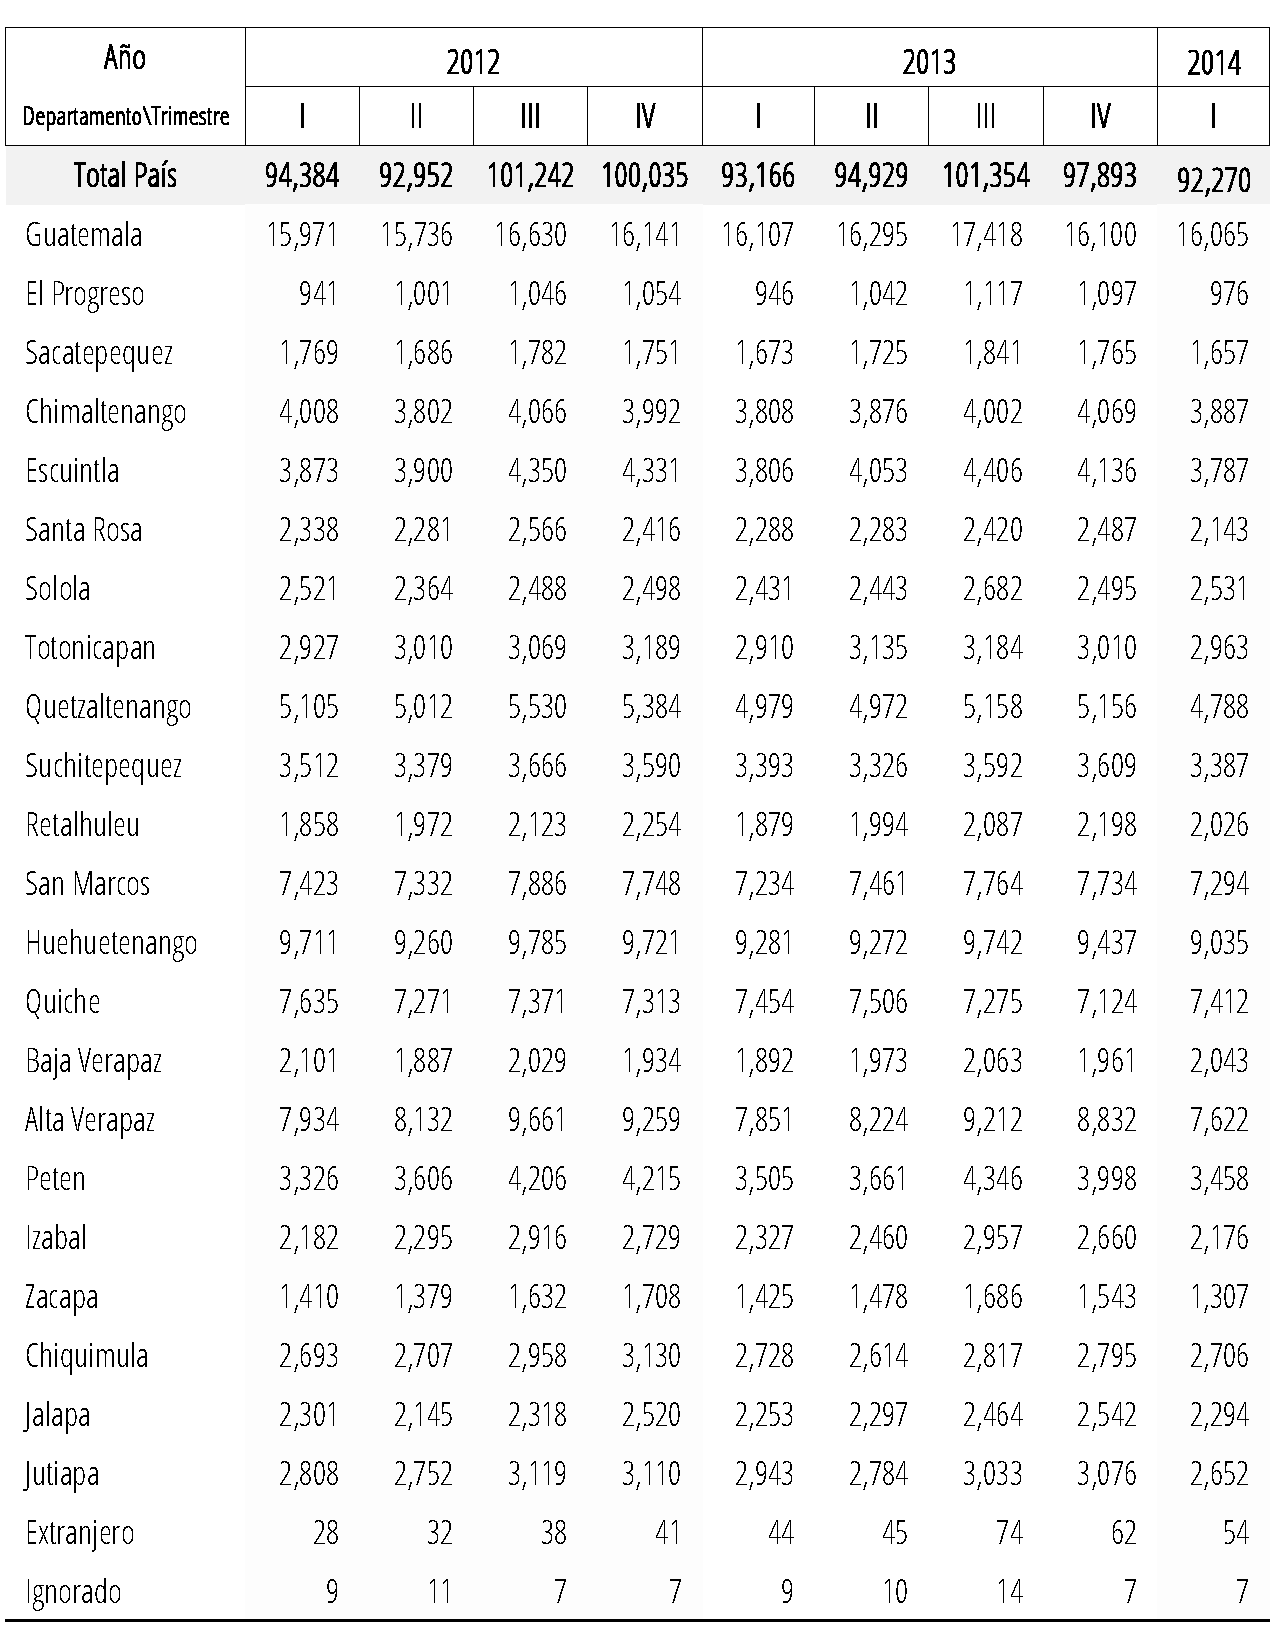
\includegraphics[width=26\cuadri]{nacimientos.pdf}}{INE, con datos del RENAP}{}}
{\columna{Defunciones por trimestre de ocurrencia, según departamento de residencia de la persona fallecida}{}{}{2}{}{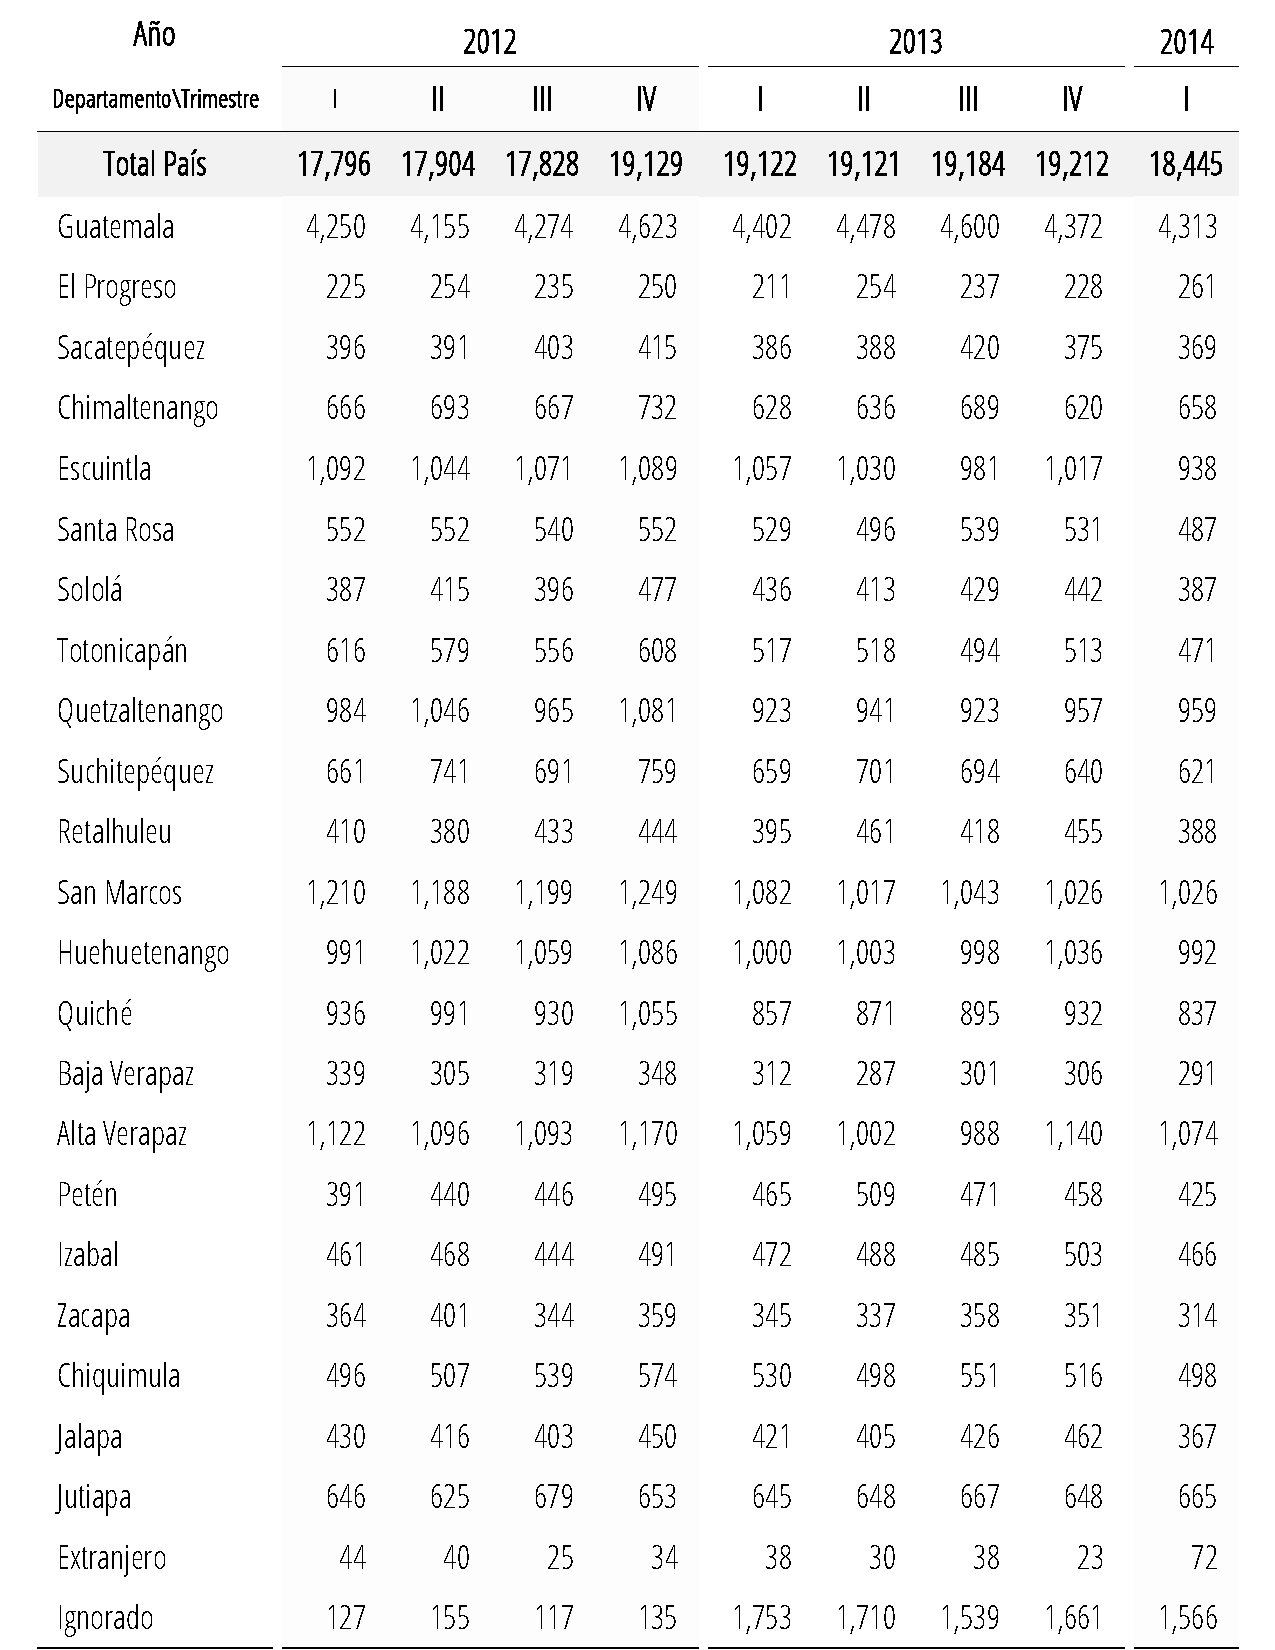
\includegraphics[width=26\cuadri]{defunciones.pdf}}{INE, con datos del RENAP}{}}

\hojados{\columna{Defunciones fetales por trimestre de ocurrencia, según departamento de residencia de la madre}{}{}{3}{}{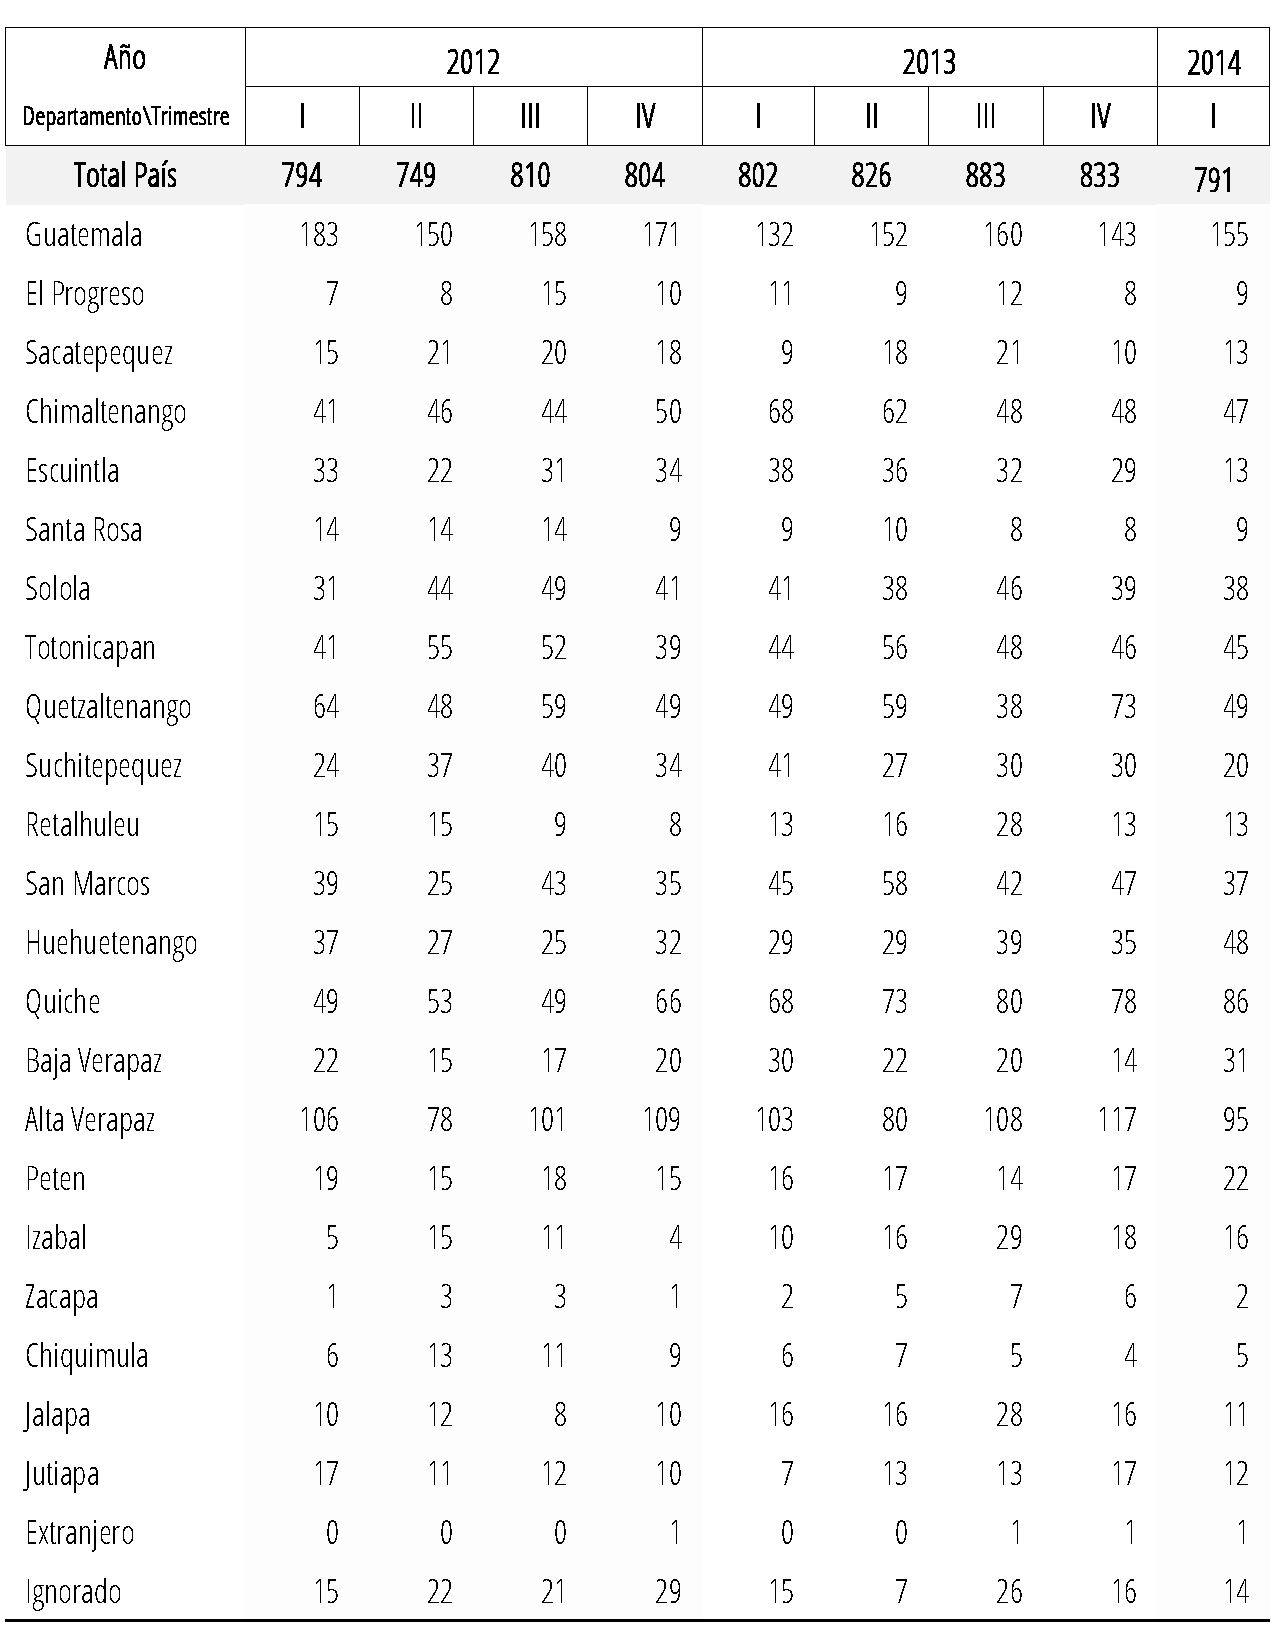
\includegraphics[width=26\cuadri]{defuncionesfetales.pdf}}{INE, con datos del RENAP}{}}

{\columna{Matrimonios por trimestre, según departamento de ocurrencia}{}{}{4}{}{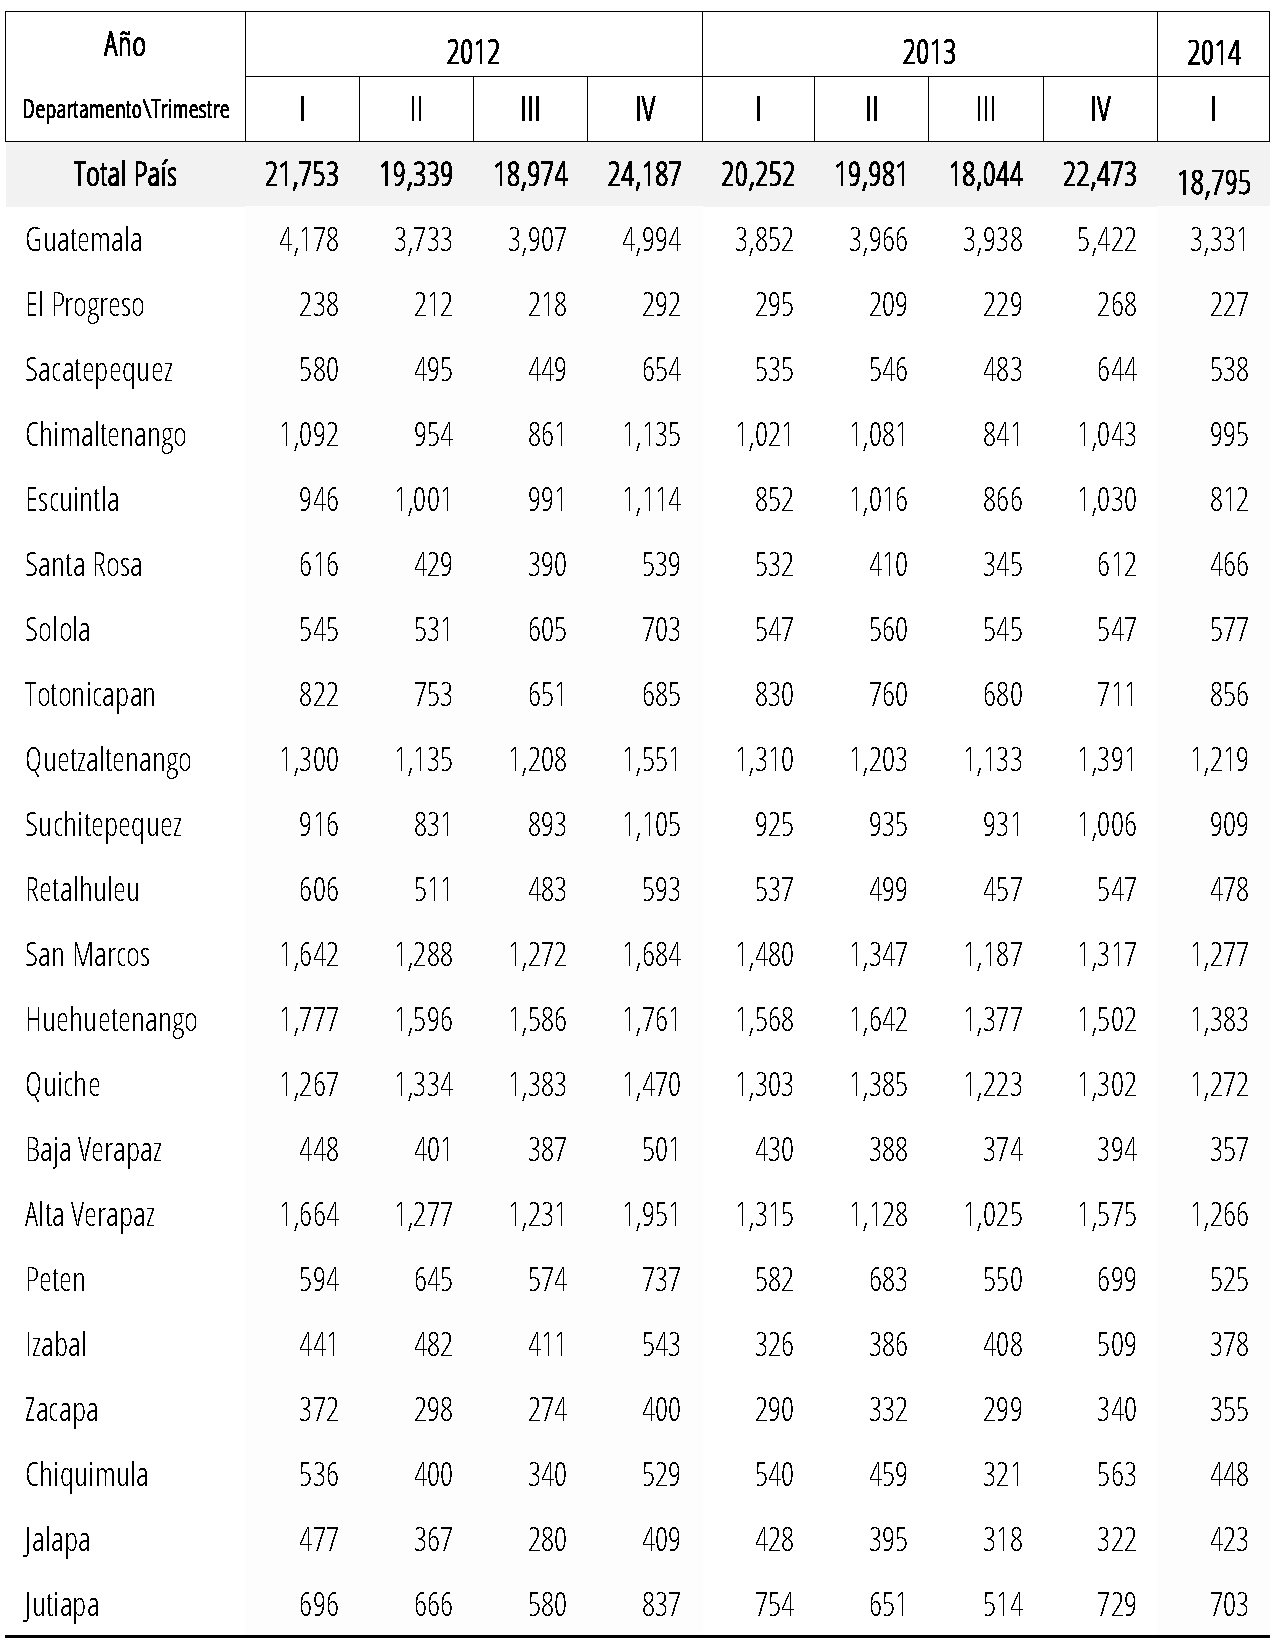
\includegraphics[width=26\cuadri]{matrimonios.pdf}}{INE, con datos del RENAP}{}}

\hojados{\columna{Divorcios por trimestre, según departamento de ocurrencia}{}{}{5}{}{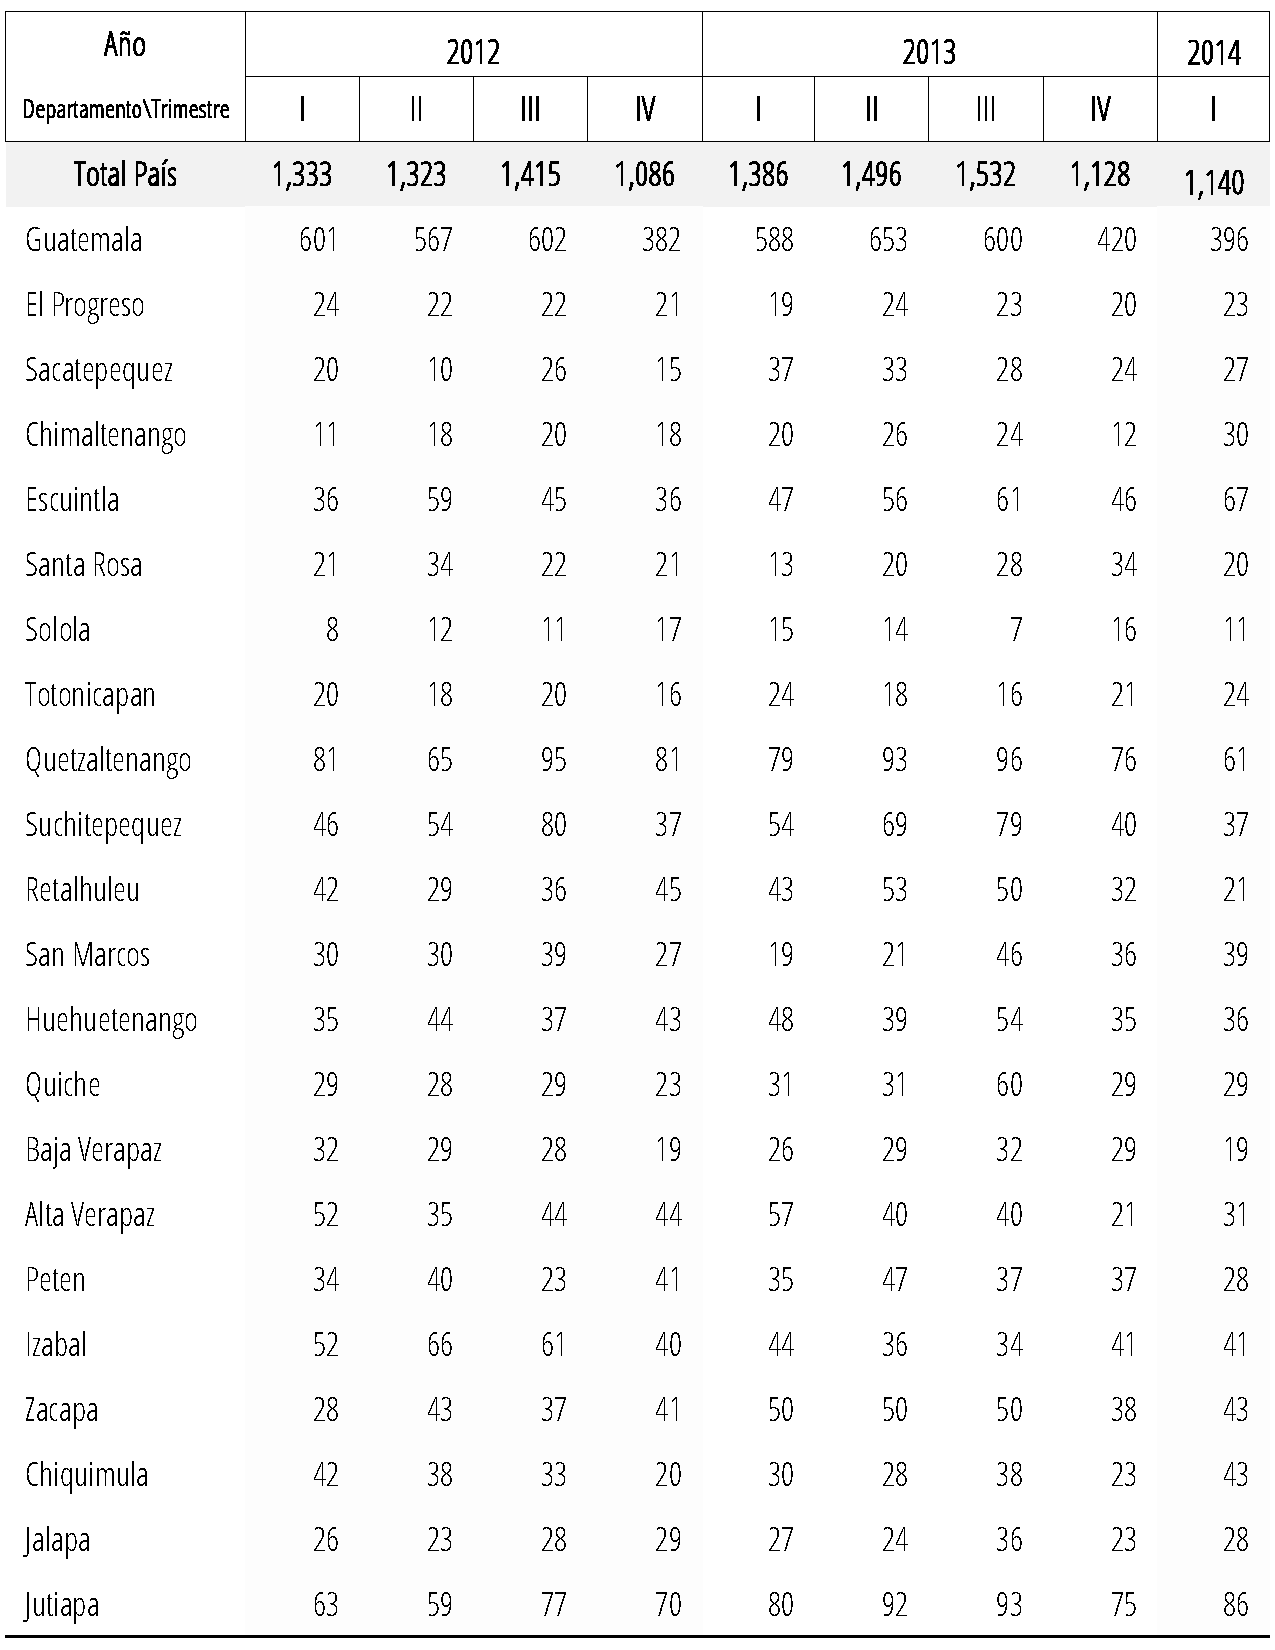
\includegraphics[width=26\cuadri]{divorcios.pdf}}{INE, con datos del RENAP}{}}




\INEchapter{TABLAS DE VARIACIONES}{TABLAS DE VARIACIONES }{ }{ }
\hojados{\columna{Nacimientos}{}{}{1 }{ } {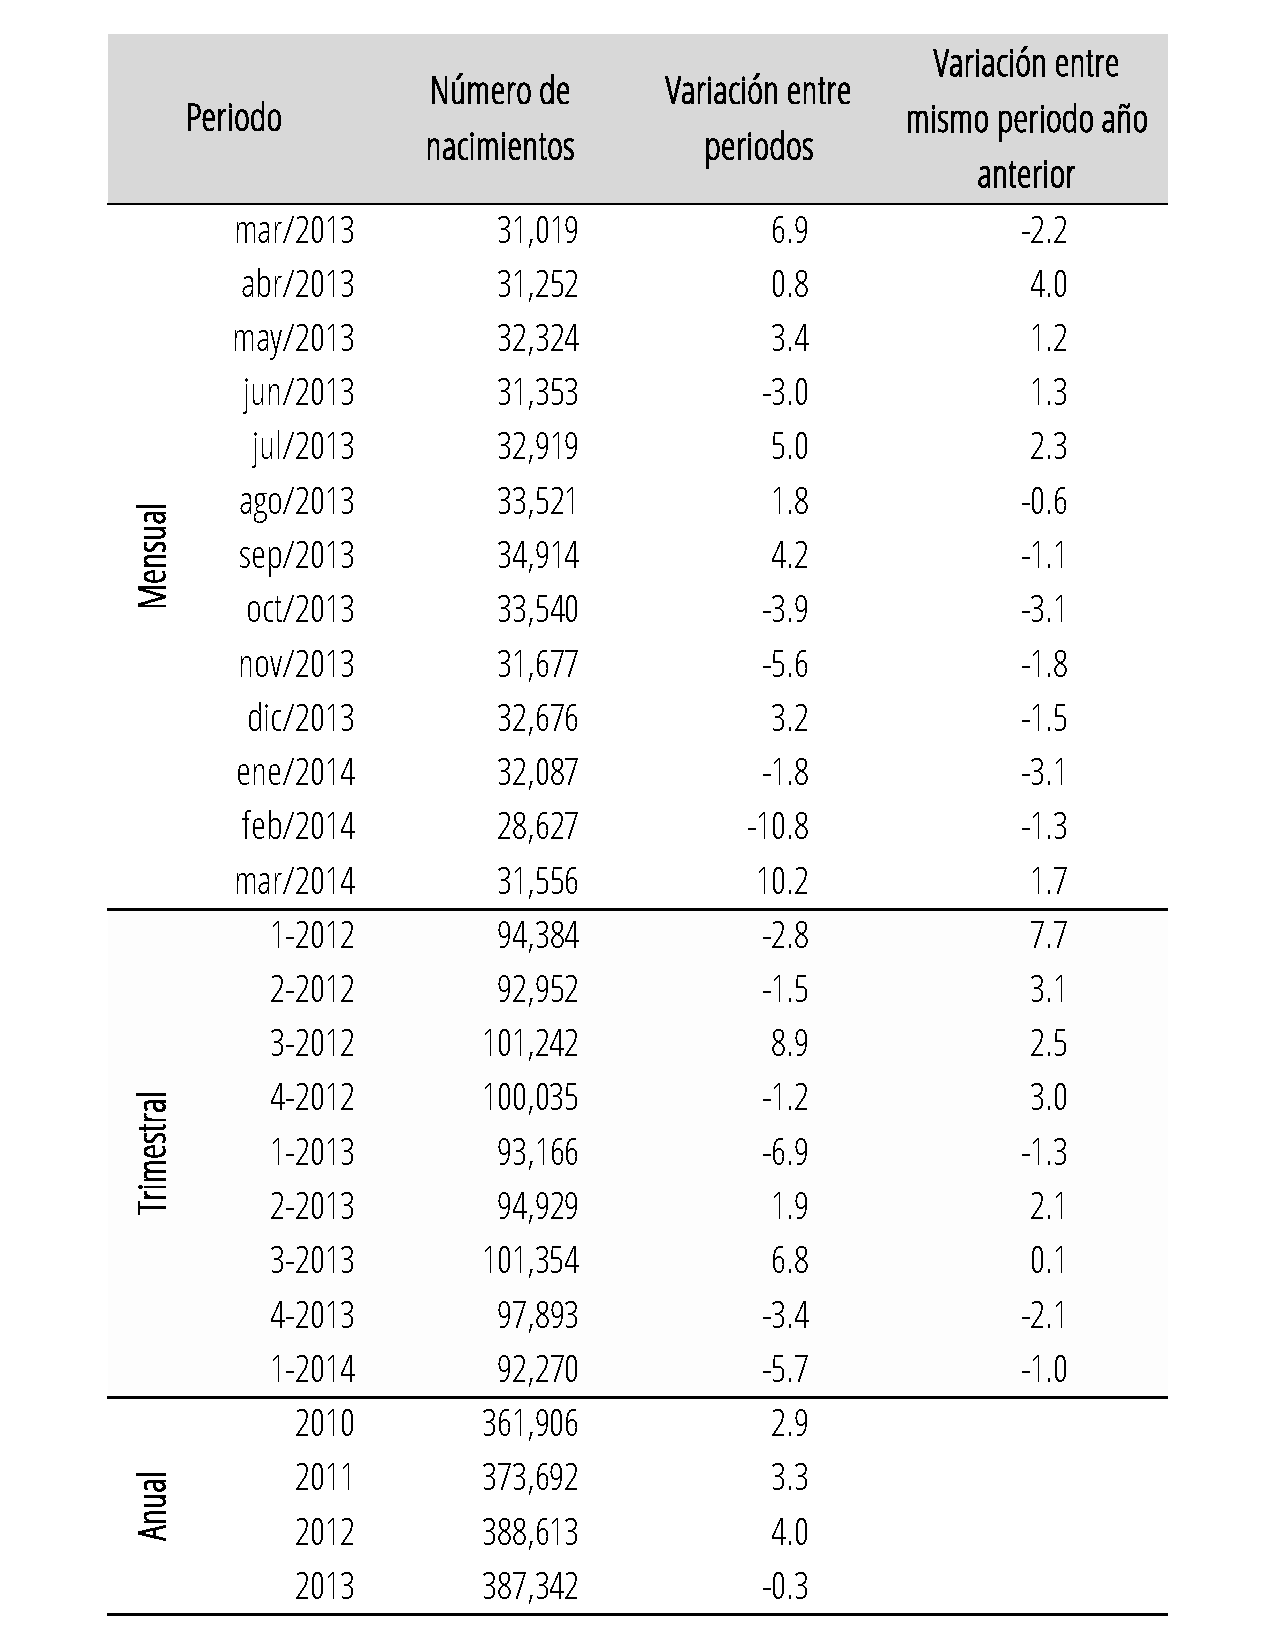
\includegraphics[width=26\cuadri]{vnacimientos.pdf}}{INE, con datos del RENAP.}{\notitasin{Los datos del año 2014 se presentan como preliminares y serán ajustados con los registros tardíos.}}}
{\columna{Defunciones}{}{}{2}{}{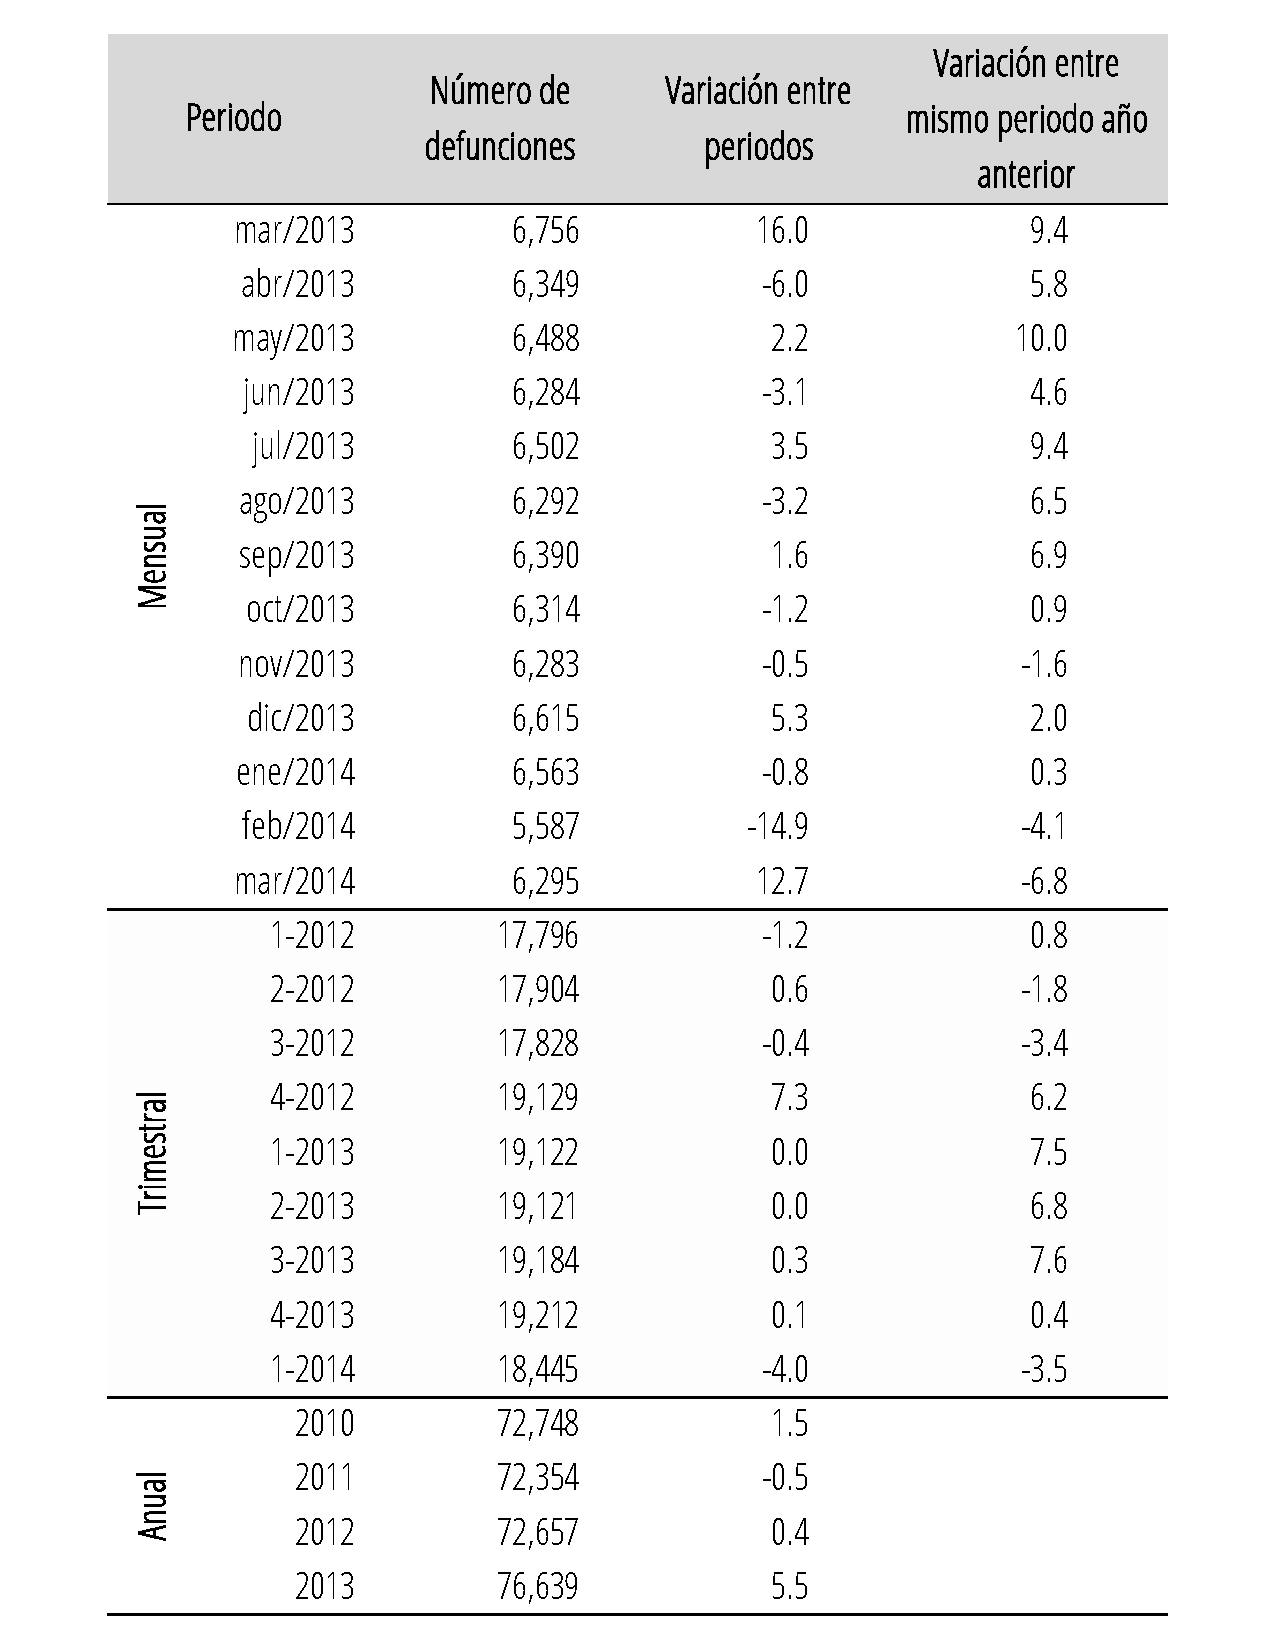
\includegraphics[width=26\cuadri]{vdefunciones.pdf}}{INE, con datos del RENAP.}{\notitasin{Los datos del año 2014 se presentan como preliminares y serán ajustados con los registros tardíos.}}}
\hojados{\columna{Defunciones fetales}{}{}{1 }{ } {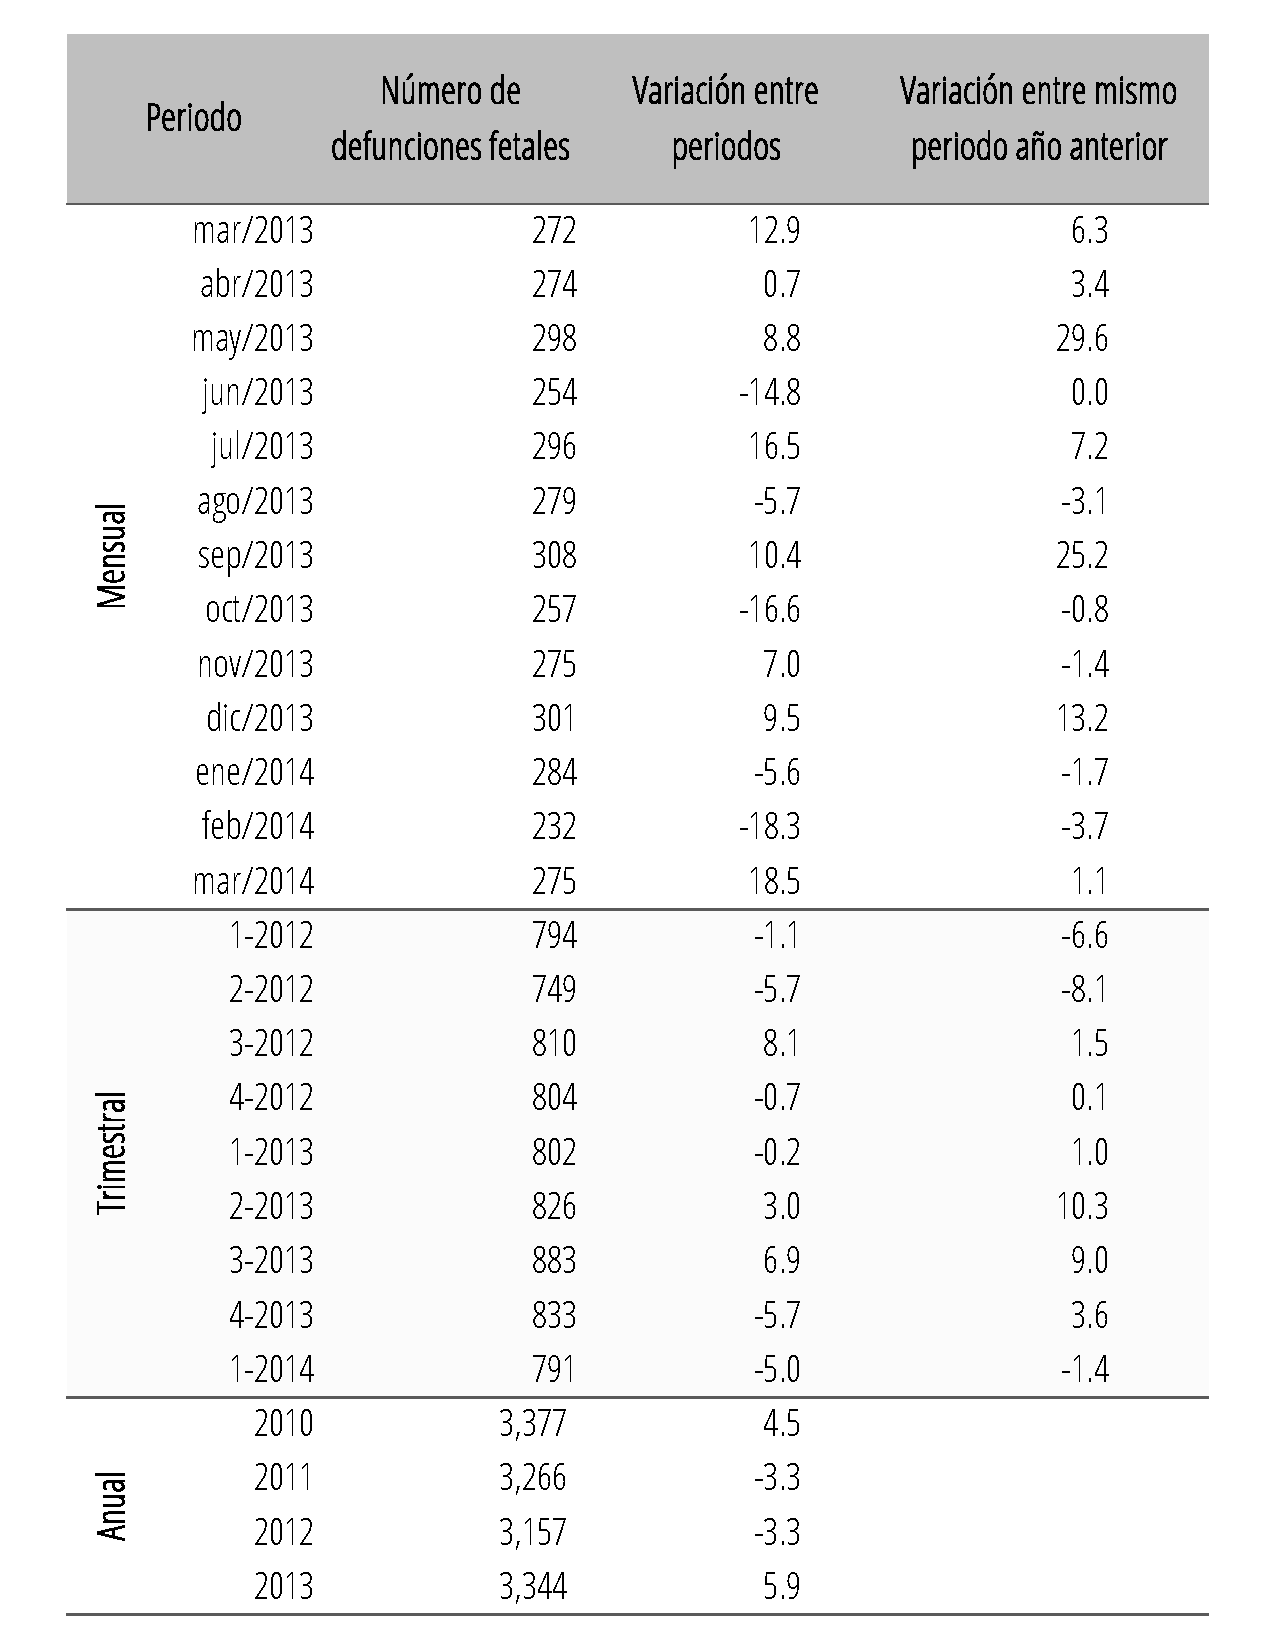
\includegraphics[width=26\cuadri]{vdefuncionesfetales.pdf}}{INE, con datos del RENAP.}{\notitasin{Los datos del año 2014 se presentan como preliminares y serán ajustados con los registros tardíos.}}}
{\columna{Matrimonios}{}{}{2}{}{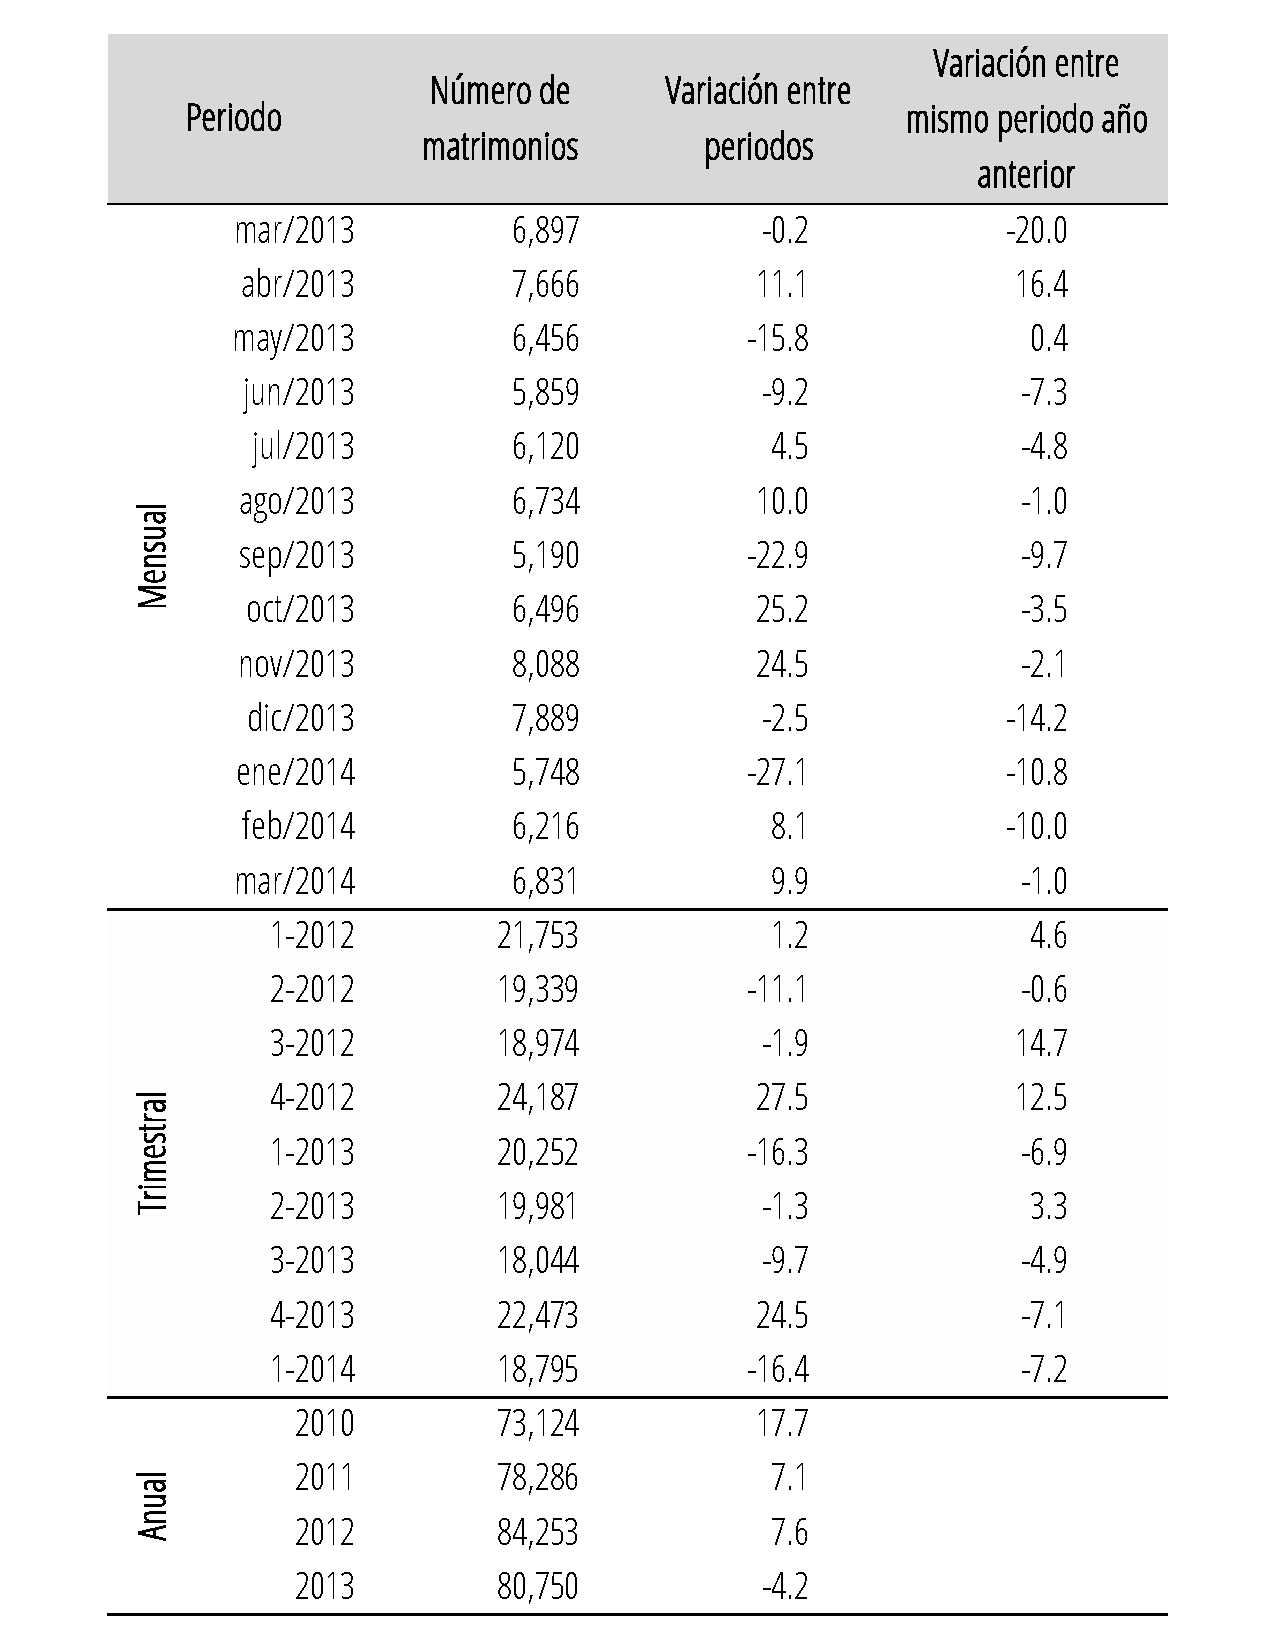
\includegraphics[width=26\cuadri]{vmatrimonios.pdf}}{INE, con datos del RENAP.}{\notitasin{Los datos del año 2014 se presentan como preliminares y serán ajustados con los registros tardíos.}}}
\hojados{\columna{Divorcios}{}{}{1 }{ } {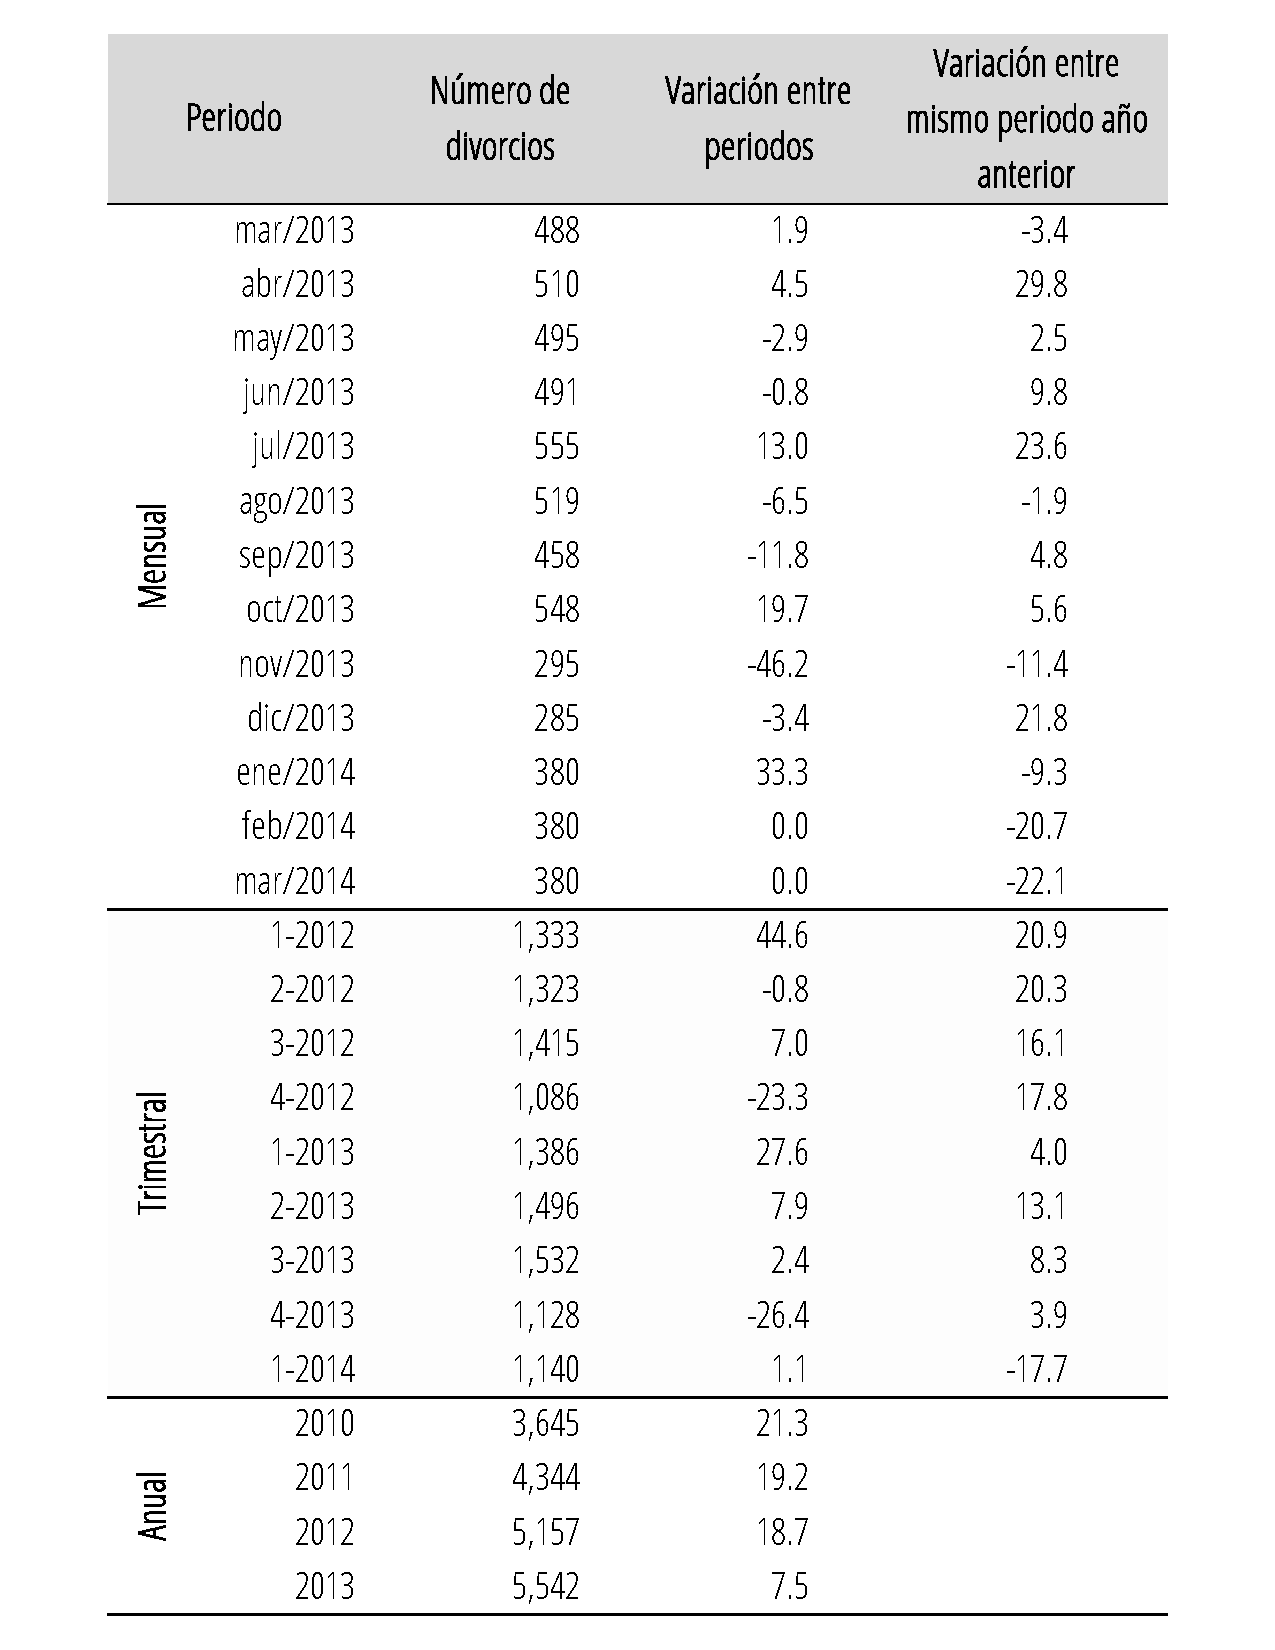
\includegraphics[width=26\cuadri]{vdivorcios.pdf}}{INE, con datos del RENAP.}{\notitasin{Los datos del año 2014 se presentan como preliminares y serán ajustados con los registros tardíos.}}}



\end{document}